% this file demonstrates the use of the NRELreport style file.

% ---------------
% PREAMBLE
% ---------------
%\documentclass[tagged]{NRELreport}
%\documentclass[tagged,11pt]{NRELarticle}
\documentclass[10pt]{article}
\usepackage{tabularx}
\usepackage{units}
\usepackage{array}
\usepackage{setspace}
\usepackage{subcaption}
\usepackage{graphics,graphicx,color}
\usepackage{amsmath,amsthm,amssymb,amsfonts,stmaryrd,latexsym}
\usepackage{hyperref}
%--------------------------------------------------------------------%
% Comment out for NREL class
\usepackage[margin=1in]{geometry}
\usepackage[format=hang,labelfont={small,bf},textfont=small]{caption}
\usepackage[square,comma,numbers,sort&compress]{natbib}
%--------------------------------------------------------------------%
\graphicspath{{figs/}}
\DeclareGraphicsExtensions{.pdf}
\setstretch{1.1}
% -----------------------------------
%\addbibresource{offshore.bib}
% -----------------------------------
% DOCUMENT PROPERTIES
% -----------------------------------
\title{Floating Offshore Wind Turbine Substructure Design and
  Sensitivity to Tower Top Weight with a Hydrostatic-based Systems
  Design Tool}
\author{Garrett E. Barter, Amy Robertson, Walter Musial, and Senu Sirnivas}
\date{September 30, 2018}
% -------------------------------------
% CUSTOMIZATIONS
% -------------------------------------

\newcommand{\mytt}[1]{\texttt{\scriptsize #1}}
\newcommand{\mcal}[1]{\mathcal{#1}}
\newcommand{\mbb}[1]{\mathbb{#1}}
\newcommand{\mbf}[1]{\mathbf{#1}}
\newcommand{\sbf}[1]{\boldsymbol{#1}}
\newcommand{\dd}[2]{\frac{\textrm{d} #1}{\textrm{d} #2}}
% 'st' 'nd' 'rd' 'th' superscripts for numbers
\newcommand{\first}{\raise.5ex\hbox{\small st}}
\newcommand{\second}{\raise.5ex\hbox{\small nd}}
\newcommand{\third}{\raise.5ex\hbox{\small rd}}
\newcommand{\fourth}{\raise.5ex\hbox{\small th}}
\renewcommand{\th}{\raise.5ex\hbox{\tiny th}}

%--------------------------------------------------------------------%
%\setstretch{1.3}
%--------------------------------------------------------------------%

% -------------------------------------
% DOCUMENT STARTS HERE
% -------------------------------------
%\lstset{language=Python,columns=fullflexible,keepspaces=true,breaklines=true,basicstyle=\scriptsize\ttfamily,mathescape=true,aboveskip=-6pt,belowskip=0pt}
%\setcounter{tocdepth}{1}
\begin{document}

%\frontmatter
%\mainmatter
\maketitle
\section*{Abstract}
This work introduces \textit{FloatingSE}, the floating offshore wind
turbine substructure cost, sizing, and analysis module in the Wind-Plant
Integrated System Design \& Engineering Model (WISDEM) framework.  The
tool generalizes its geometry parameterization so as to use the same set
of variables to describe spars, semisubmersibles, tension leg platforms
(TLPs), and hybrids of those archetypes.  Design evaluation is done by
the application of existing codes and standards, hydrostatic principals,
and simple beam finite element static structural analysis.  With other
multidisciplinary WISDEM modules, the inclusion of \textit{FloatingSE}
enables the vertical simulation of a floating offshore wind turbine,
even a whole plant if desired.  To showcase this capability, a two-step
optimized-based analysis was carried out.  First, three different
substructures, a spar, semisubmersible, and TLP, were designed beneath a
\unit[10]{MW} reference turbine. Second, a design sensitivity study was
conducted where mass in the nacelle was parametrically removed, to
simulate the addition of a novel drivetrain or generator technology, and
the design re-optimized.  The derived sensitivities were used to
ascertain the break-even cost rate of the new technology that reduces
the drivetrain mass, but at a cost premium (\$1,000 for the spar, \$450
for the semisubmersible, and \$100 for the TLP).  Another noteworthy
observation is that mass is poor surrogate for cost in optimization
studies, a convention frequently used in conceptual design studies.  Due
to the many simplifying assumptions and low-fidelity analysis, the
optimized design and sensitivity values come with many caveats and are
subject to change following future development.

\section{Introduction}
\label{sec:intro}

The US offshore wind gross resource potential is over
\unit[2000]{GW}\footnote{The technical offshore wind resource potential
  that is greater than \unit[7]{m/s} annual average wind speed was
  calculated to be \unit[2058]{GW}, considering all ocean and lake areas
  less than \unit[1000]{m} depth.}, much of which is located near highly
populated coastal load centers\footnote{Excludes areas in the Great
  Lakes deeper than \unit[60]{m} because technology for floating
  structures to survive ice conditions has not been matured yet.}
\cite{resource}.  This vast potential is distributed over a resource
area of which approximately 58\% is in water that is \unit[60]{m} deep,
or greater, and that proportion rises to 95\% on the Pacific coastline
\cite{musial-ca}. The fundamental wind turbine technology shift for
deployment in deep water is the transition to buoyant support structures
from conventional fixed-bottom support structures, which become too
costly and more technically challenging in deep water (likely greater
than \unit[50]{m}) \cite{obos}. Although floating wind turbines present
many new technical challenges, they also have many potential benefits
compared to shallow-water systems.  Wind speeds can be higher in
deep-water regions because they are further from shore, although there
are exceptions to this trend.  Siting floating projects may be easier
near large load centers such as the North Atlantic, because plants
farther from shore may have fewer environmental and human use impacts,
including viewshed issues\footnote{Musial et al 2016 found that human
  use conflict diminished from 49\% inside \unit[3]{nm} to below 8\%
  outside \unit[50]{nm}}.  Despite the distance from shore, floating
systems may also be easier to install since they have the potential to
be fully assembled at regional construction ports, commissioned at
quayside, and towed out.

Preliminary analysis suggests that, in time, floating technology has the
potential to achieve a lower cost of energy than their fixed-bottom
counterparts \cite{spatial}.  In fact, the Statoil Hywind floating plant
recorded a higher capacity factor in its first few months of operation
than its fixed-bottom brethren \cite{statoil-hywind}.  However, as a
nascent technology, the cost of floating offshore wind energy is still
high today.  Detailed modeling shows that the needed long-term cost
reductions are not likely to come from a single breakthrough
invention.  Instead, significant cost reductions will come from a
disciplined combination of complementary innovations, or a technology
cost reduction \textit{pathway}.

To produce transformational cost reductions, multiple advancements are
needed over the entire system: the turbine, tower, floating platform,
moorings, anchors, construction, and logistics.  However, the
complexities of the physics, manufacturing, installation, and operation
of floating wind turbines require a fully integrated systems engineering
and techno-economic design approach to achieve these transformational
cost reductions.   The paper outlines an initial, low-fidelity
step towards realizing this vision and an example analysis.

\subsection{Multidisciplinary Analysis and Optimization (MDAO)}
A systems engineering framework advocates for an
\textit{integrated} approach to design, where all disciplines, costs,
performance measures, and constraints are considered concurrently.
Essentially, an analysis framework for wind plants must capture the
entire power path, from the aerodynamics to the generator and grid; the
entire load path, from the nacelle through the tower and foundation; and
the entire balance sheet, from concept through decommissioning.
Executing this proposed approach in a closed-loop optimization framework
is critical to achieve superior cost and performance gains.
A graphical depiction of this idea is shown in Figure
\ref{fig:mdao}.

\begin{figure}[htbp]
  \begin{center}
    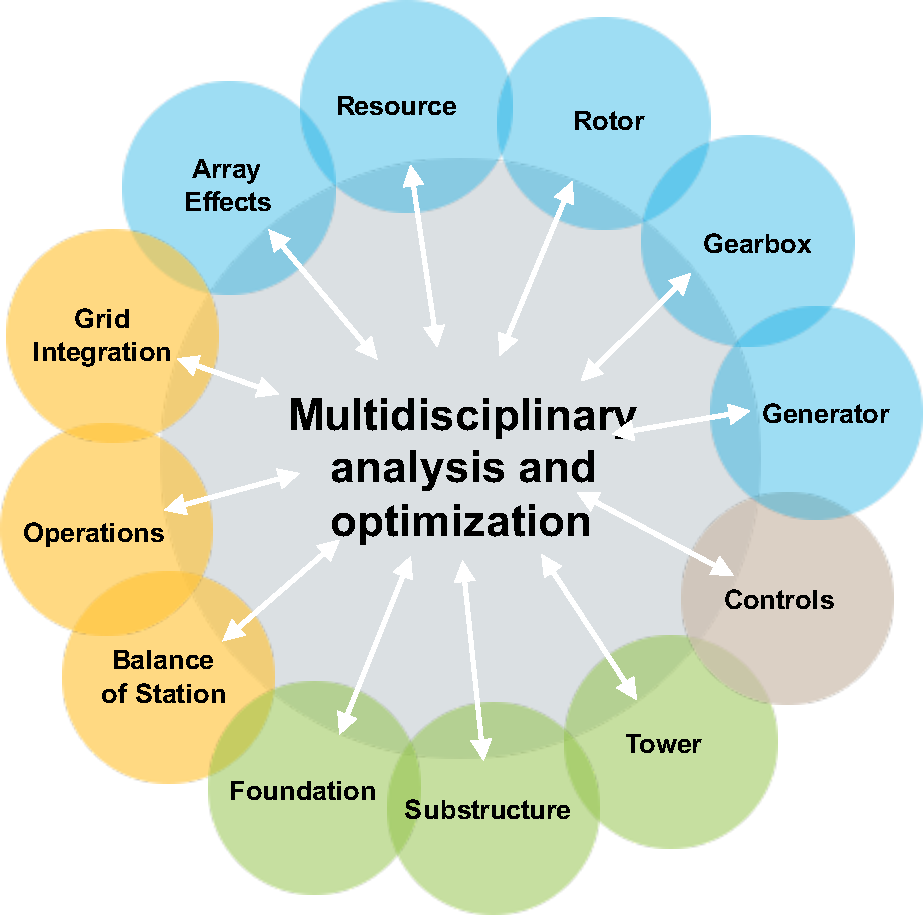
\includegraphics[width=2.5in]{mdao}
  \caption{``Integrated'' multidisciplinary design analysis and optimization
    (MDAO) approach.}
  \label{fig:mdao}
  \end{center}
\end{figure}

Multidisciplinary analysis and optimization (MDAO) would be beneficial
for all wind turbine systems, but perhaps even more so for floating
offshore systems due to their lower level of maturity, compliant nature
(motion in all six degrees of freedom), and tight inter-dependencies
among their subsystems. The stiffness and damping of the structural
members in the load path can impact the power production of the
turbine. The characteristics that minimize balance of station costs must
be integrated at the outset into the designs of the power generation and
load paths. The control systems at the turbine and plant level must
balance the demands of immediate power generation versus long-term
fatigue of the components.

MDAO has its roots in the aerospace industry with publications reaching
back into the 1960s and 1970s \citep{schmit60, haftka1977}. It grew
within aerospace and expanded to many more industries with its own
dedicated conferences and professional organizations. See
\citet{martins2013} for a more comprehensive review. With its close ties
to the aerospace industry, the wind industry was also a natural
application for MDAO practitioners. \citet{kuhn99} performed one of the
first cost-based optimizations of an offshore wind plant in 1999. Later,
\citet{dykes2011} provided a detailed review and position paper on
systems engineering and MDAO for wind energy, which triggered the
development of the Wind-Plant Integrated System Design \& Engineering
Model (WISDEM) tool. For instance, \citet{ning2014} analytically
obtained a cost of energy decrease of 5\% for land-based sites and 2\%
for offshore sites by loosening constraints on rotor tip
speed. \citet{fleming2016} showed the ability to increase the power
density of a wind farm by approximately 30\%. Concurrently,
\citet{maki2012} published one of the first system-level optimizations
of a wind turbine and found potential for a nearly 30\% decrease in the
cost of energy. \citet{ashuri2014} used MDAO principles in a system
optimization of an offshore turbine and showed a 2.3\% improvement in
levelized cost of energy (LCOE) over an NREL 5-MW reference
turbine. This work was focused on the aero-structural interactions of
the blades, rotor, and tower and had only loose coupling to wind plant
and balance-of-system (BOS) models.  \citet{bottasso2012} started
developing a research-focused systems engineering framework, with
emphasis on the rotor.  This work used multiple inner optimizations
instead of one global optimization and culminated in an excellent
summary paper by \citet{bortolotti2016}.  By most accounts, future
interest in MDAO will persist, both within the academic and industrial
wind energy community.  In fact, the number of contributors and papers
has grown so large that it was not possible to properly cite all the
interesting works in this report.

The International Energy Agency (IEA) has also recognized the need for
systems engineering tools. A research task has recently been initiated
under the IEA, Wind Task 37 – Wind Energy Systems Engineering:
Integrated Research, Design, and Development.  This task aims to
coordinate international research activities, towards the analysis of
wind power plants as holistic systems by improving the practice and
application of systems engineering to wind energy research and
development.  A couple notable publications from this effort include
\citet{perez2016}, describing a research roadmap for MDAO in wind
energy, and \citet{perez2018}, which proposed a reference offshore wind
plant, designed with MDAO.

Short of considering the entire offshore turbine, a number of authors
have focused on optimization of one or more components using MDAO
techniques. Much of this work has centered on the substructure,
including both fixed-bottom jackets/monopiles and floating substructures
(see \citep{muskulus2014}). One prominent example was the LIFES50+
consortium, which attempted to develop innovative substructure designs
to lower the LCOE of floating offshore wind plants using many MDAO
principles \citep{lifes50-framework}. LIFES50+ has examined four
candidate floating concepts and is pursuing a rigorous model and
experimental performance validation of two down-selected designs. In
addition, \citet{damiani2016} showed the application of a systems
engineering tool to optimize the cost of building a fixed-bottom jacket
structure at various locations in the United States. The optimization
itself was only focused on the mass of the structure, but the LCOE of
the optimized designs were compared, including the costs of
manufacturing and installation. Similarly, \citet{haafele2016} examined
the optimization of a jacket substructure using a cost function that
includes the raw material costs as well as contributions of
manufacturing, transport, and installation, and they found the ability
to reduce costs by over 20\%. Finally, \citet{lozano2011} used the
TOPSIS (Technique for Order Preference by Similarity to Ideal Solution)
tool to incorporate both environmental and lifetime cost considerations
to determine the most appropriate support structure for an offshore wind
site. \citet{karimi2017} used a genetic algorithm to mix and match
geometry components to create optimal hybrid substructures.  This is the
work that most closely resembles the analysis presented in this paper,
with some differences, of course.

\subsection{Role of Experience in MDAO for Floating Offshore Wind Energy}
One common misconception with MDAO is that the design framework and
optimization algorithms replace the engineer and dilute the value of
experience.  For the application of floating offshore wind energy
systems, this statement is far from the truth.  The hierarchy of design
criteria that sequentially narrow the design space is shown in Figure
\ref{fig:tradespace}.  First, to move to designs that will physically
survive and produce net energy, international consensus-based standards
through the International Electrotechnical Commission (IEC) and American
Petroleum Institute (API) must be met.  These standards are encapsulated
in design frameworks, such as the one proposed here, through
constraints.  Most of the floating wind prototype designs would probably
meet a basic set of certification requirements, even though
internationally recognized standards are still in development.  However,
even a fully mature certification process would serve mainly to reduce
deployment risk, not drive innovation or push the technology towards
lower-cost designs.  This is the motivation for the second step in
Figure \ref{fig:tradespace}, which arrives at a smaller region of the
tradespace that encompasses the designs with the potential to be
cost-competitive.  Concepts in this space satisfy a rubric of criteria
focused on lowering cost learned via experience.  Meaning, the
real-world lessons gained from floating turbine prototypes and tank
tests are also imbued into the design framework.  Experience manifests
itself in the underlying architecture of the design framework, its
parameterization of the geometry, the constraints, design variables, and
other options available to the user.  Without this experience, the
optimized designs that come out of the framework would likely fall to
gain credibility among the offshore wind community.  Once the tradespace
is sufficiently narrowed by standards and experience, then the
optimization is used to maximize performance This allows the engineers
and optimization tools to focus their resources on the region of the
tradespace that has the greatest cost-reduction potential.

\begin{figure}[htbp]
  \begin{center}
    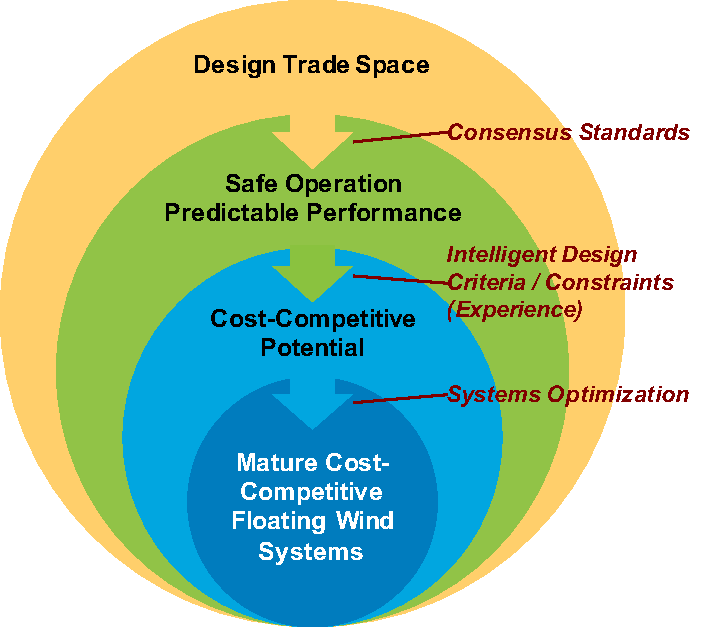
\includegraphics[width=3in]{tradespace}\\
    \caption{Narrowing the tradespace to accelerate floating system optimization.}
    \label{fig:tradespace}
  \end{center}
\end{figure}


\subsection{Modeling Framework}
WISDEM is selected as the platform for development of the design
framework envisioned in this paper.  The Wind-Plant Integrated System
Design and Engineering Model (WISDEM), developed by NREL, is a set of
integrated modules that creates a virtual, vertically integrated wind
plant. The models use engineering principles for conceptual design and
preliminary analysis, and link to financial modules for LCOE
estimation. The modules can be thought of as templates, in that they can
be easily tweaked for any analysis question by considering any variable
a design variable and any output an optimization objective or
constraint. The WISDEM modules are built around the OpenMDAO library \citep{openmdao},
allowing for the modules to be exercised individually for component
analysis or in unison for turbine or plant level studies.  

\begin{figure}[htbp]
  \begin{center}
    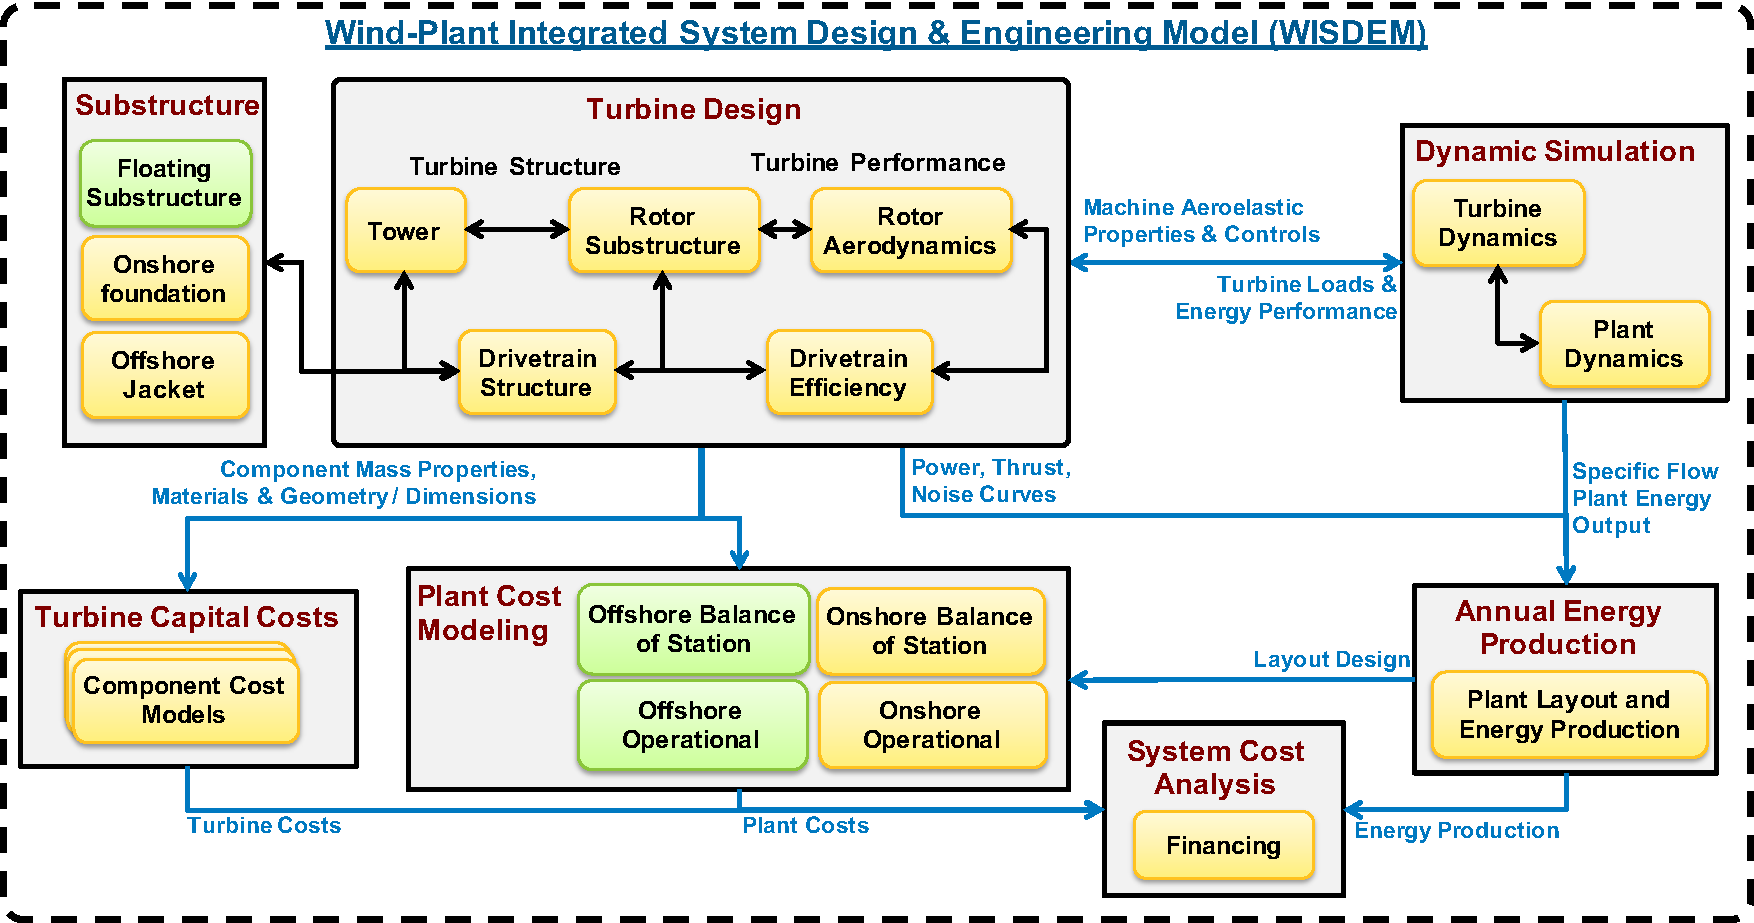
\includegraphics[width=5in]{new_wisdem}\\
    \caption{Update of WISDEM to include floating wind design modules.
      Yellow denotes an existing module and green colored modules are
      those that will be developed in this effort (note that
      fixed-bottom offshore turbines and support structures are already
      modeled).}
    \label{fig:wisdem}
  \end{center}
\end{figure}

WISDEM and the OpenMDAO library provide a solid platform from which to
develop the necessary tools for a system-level optimization methodology
for floating wind systems.  A diagram of WISDEM, with highlights of the
new modules added in course of this project is shown in Figure
\ref{fig:wisdem}.  WISDEM accounts for most of the turbine disciplines
and components involved, except most notably the floating substructures.
At the plant level, the balance of station economics for floating wind
systems from concept through decommissioning was incorporated in WISDEM
from other another in-house NREL model.  No current open-source offshore
operations and maintenance module suitable for use in WISDEM is
currently available, but development of one is part of future plans.

The key addition to WISDEM to enable floating offshore wind energy
systems to be included in its framework is the creation of the
\textit{FloatingSE} module.  This module handles conceptual cost and
sizing design of floating substructures by parameterizing the geometry
and analyzing candidate configurations with low-fidelity approximations
of loads, stress analysis, mooring system behavior, stability criterion,
and compliance with existing codes and standards.  A flow chart of the
key analysis steps and tools is shown in Figure \ref{fig:floatingse}.
\textit{FloatingSE} is made available to the broader community via
GitHub as an open-source mode.

\begin{figure}[htbp]
  \begin{center}
    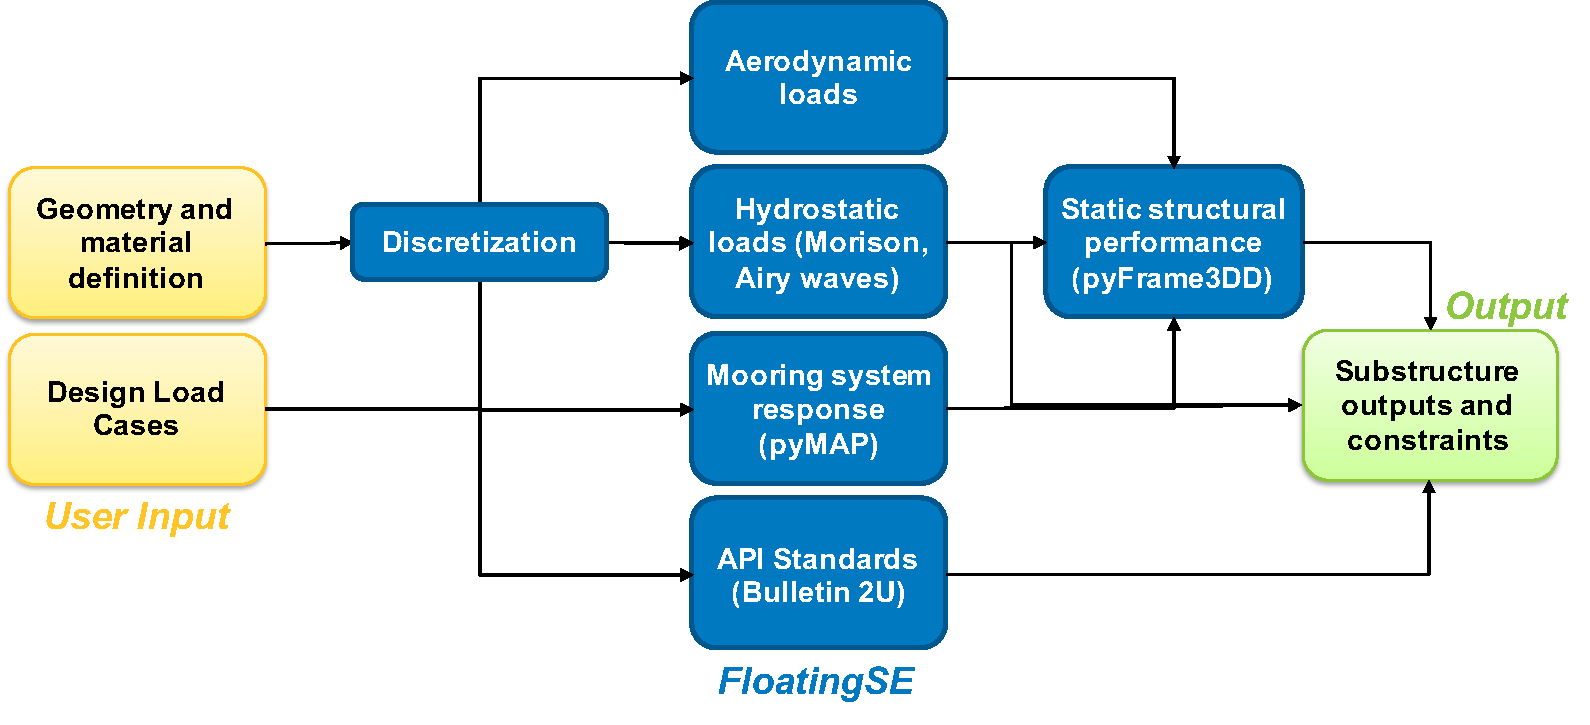
\includegraphics[width=4.5in]{floatingse}\\
    \caption{Analysis steps and tools in \textit{FloatingSE}, the floating substructure design module within WISDEM.}
    \label{fig:floatingse}
  \end{center}
\end{figure}

The next two sections of the paper present the details of
\textit{FloatingSE}.  Section \ref{sec:geom} describes the geometry
parameterization in a general manner to enable conceptual design
exploration of both classical and novel configurations.  Section
\ref{sec:theory} then describes how a design configuration is evaluated
in \textit{FloatingSE}, through the analysis flow shown in Figure
\ref{fig:floatingse}.

\subsection{Analysis Overview}
The final two sections of the paper feature an optimization-based design
and sensivitiy study meant to showcase the capabilities of
\textit{FloatingSE} within the WISDEM framework.  The application
features the conceptual design of three classical floating substructures
with \textit{FloatingSE}, guided only by design variable bounds and
constraints.  After showcasing the designs, a sensitivity study is
conducted where the mass of the nacelle is parameterically changed, and
the substructure designs re-optimized.  The optimization problem
formulation and solution methodology for the design and sensitivity
studies is described in Section \ref{sec:opt}.  The results of the
studies, both the conceptual designs of floating turbine substructures
and the sensitivity study, is presented in Section \ref{sec:results}.

The analysis presented here helps to quantify
the value of weight reduction in floating offshore wind turbines.
Weight minimization, and a cost premium, is a classic cost-benefit
tradeoff study that is especially germane to floating offshore wind
energy systems.  Parameterically changing the weight of the nacelle is a
surrogate for new drivetrain and generator technologies or innovations
that offer to reduce the weight of these components at a cost premium.
Without a full systems framework, it is difficult for the engineer to
make such a tradeoff.  Thus, the study here teases some of the types of
questions that could be posed and answered with the WISDEM framework to
address some of the open questions and challenges for floating offshore
wind energy systems.

\chapter{Geometry}
\label{sec:geom}
This section describes the variables and methods used to parameterize
the substructure geometry in \textit{FloatingSE}.  Typically,
substructure designs have fallen into three classical regimes, which are
shown in Figure \ref{fig:archetype}, each of which attains static stability
through different physical mechanisms.  A spar derives its stability from a
deep drafted ballast.  A semisubmersible derives its stability from
distributed waterplane area, achieved with offset columns spread evenly
around a main column or central point.  A tension leg platform (TLP) uses taut
mooring lines for its stability.

\begin{figure}[htbp]
  \begin{center}
    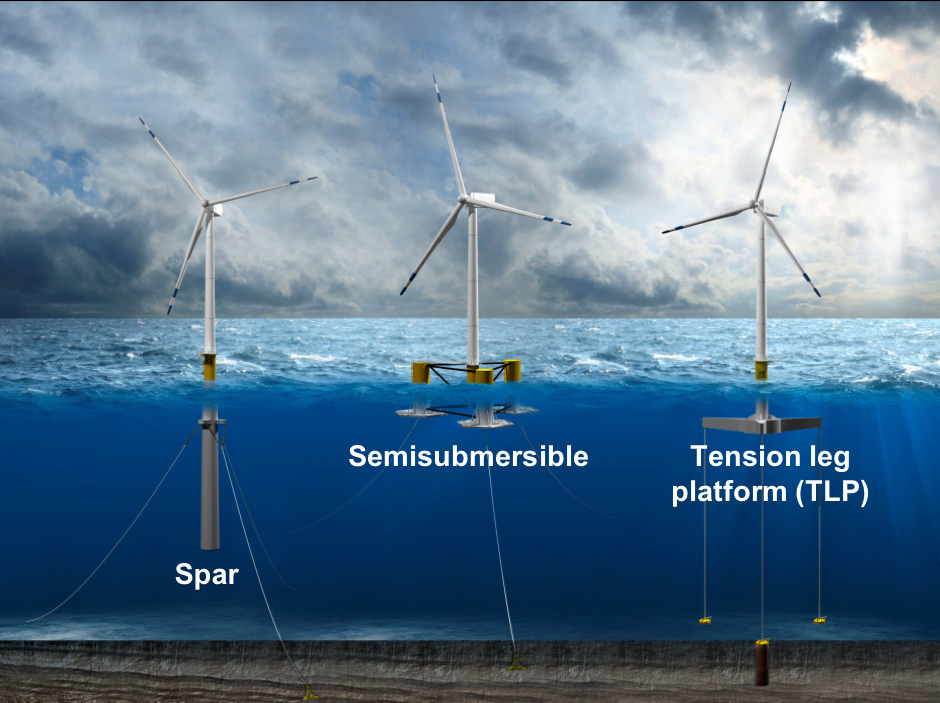
\includegraphics[width=3.75in]{archetypes}
    \caption{Three classical designs for floating turbine substructures.}
    \label{fig:archetype}
  \end{center}
\end{figure}

Similar to \citet{karimi2017}, care was taken to parameterize the
substructure in a general manner, so as to be able to use the same set
of design variables to describe spars, semisubmersibles, TLPs, and
hybrids of those archetypes.  The intent is that this modular approach
to substructure definition will enable rapid analysis of the majority of
designs currently proposed by the floating wind development community,
whether classical or novel in nature.  Furthermore, generalizing the
substructure definition also empowers the optimization algorithm to
search a broad tradespace more efficiently by moving fluidly from one
region to another.

With that intent in mind, the general configuration of a spar-type
substructure is shown in Figure \ref{fig:diagram}, with nomenclature
borrowed from the field of naval architecture.  A semisubmersible
configuration would have a similar diagram, but with multiple offset
columns connected with pontoon elements.  A TLP might look similar to a
spar or semisubmersible, with taut mooring lines instead of the catenary
ones shown.

\begin{figure}[htb]
  \begin{center}
    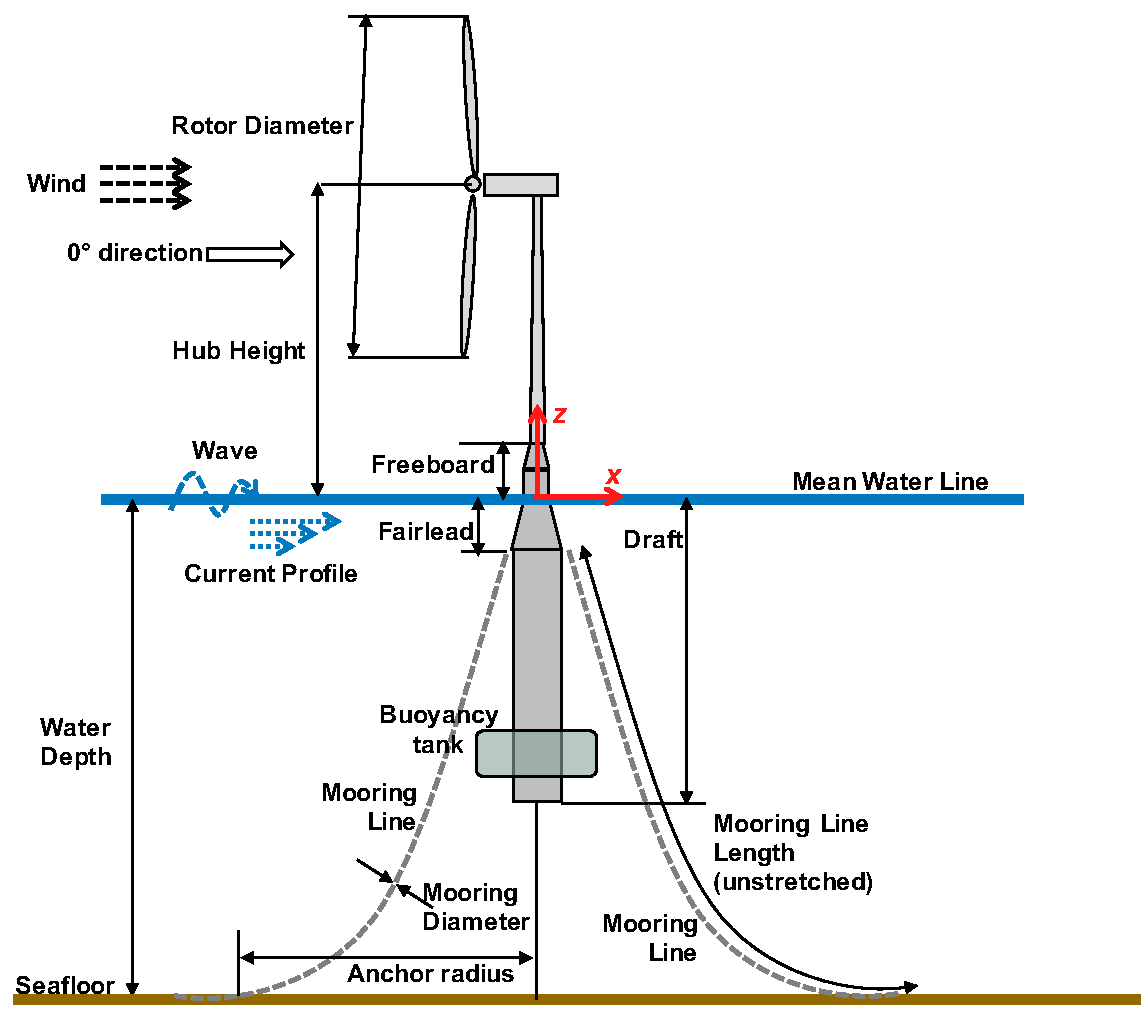
\includegraphics[width=5in]{diagram}
    \caption{Geometry parameterization with common wind turbine and
      naval architecture conventions.}
    \label{fig:diagram}
  \end{center}
\end{figure}

\section{Tapered Cylinders (Vertical Frustums)}
A number of typical floating substructure designs, such as the spar or
semisubmersible, contain vertically oriented columns.  In
\textit{FloatingSE}, these columns are
assumed to have a circular cross-section making them, formally, vertical
frustums.  These frustums are assumed to be ring-stiffened to support
the buckling loads inherent in a submerged support structure.  The
number of columns, their geometry, and the ring stiffeners are
parameterized in the \textit{FloatingSE} module according to the
diagrams in Figures \ref{fig:diagram} and \ref{fig:column}.  The main
column is assumed to be centered at $(x=0, y=0)$, directly underneath the
turbine tower (note that off-centered turbines are not yet supported).
Other columns are referred to as \textit{offset} columns, and are
assumed to be evenly spread around the main column.  The material of the
vertical columns is currently assumed to be ASTM 992 steel.
Future developments will include the option to select one of multiple
material options for each section in each cylinder.

\begin{figure}[htb]
  \begin{subfigure}[b]{0.38\linewidth}
    \centering 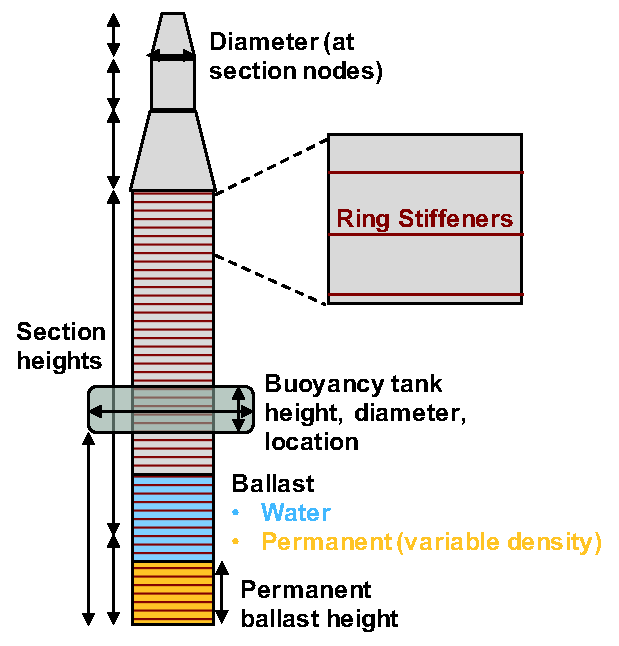
\includegraphics[width=2.2in]{colGeom}
    \caption{Vertical column of frustums}
  \end{subfigure}
  \begin{subfigure}[b]{0.29\linewidth}
    \centering 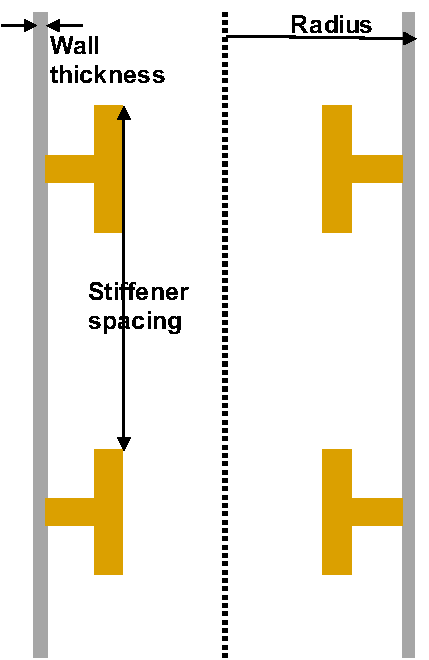
\includegraphics[width=1.8in]{stiffenerCut}
    \caption{Vertical cross-section}
  \end{subfigure}
  \begin{subfigure}[b]{0.29\linewidth}
    \centering 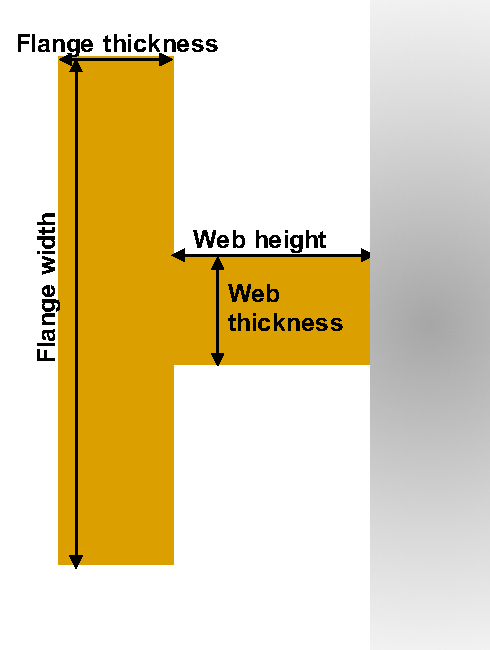
\includegraphics[width=1.8in]{stiffenerZoom}
    \caption{Ring stiffener geometry}
  \end{subfigure}
  \caption{Vertical frustum geometry parameterization.}
  \label{fig:column}
\end{figure}

\section{Discretization}
To allow for varying geometry parameters along the length of
substructure columns, the larger components are divided into sections.
The user may specify the number of overall sections, $n_s$ and the
geometry of each section.  Some of the geometry parameters are tied to
the nodes that bracket each section, such as column diameter and wall
thickness, with linear variation between each node.  Other parameters
are considered constant within each section, such as the spacing between
ring stiffeners.  The number of sections should resemble the physical
number of cans or sections used in the manufacturing of the real
article.

\subsection{Ballast}
Stability of substructure columns with long drafts can be enhanced by
placing heavy ballast, such as magnetite iron ore, at their bottom
sections.  The user can specify the density of the permanent ballast
added and the height of the ballast extent within the column.  Variable
ballast, as opposed to permanent ballast, is water that is added or
removed above the permanent ballast to achieve neutral buoyancy as the
operating conditions of the turbine change.  A discussion of variable
water balance in the model is found in Section \ref{sec:static}.

\subsection{Buoyancy Tanks (and Heave Plates)}
Buoyancy tanks are modeled as a collar around the column and are not
subject the same taper or connectivity constraints as the frustum
sections.  They therefore offer added buoyancy without incurring as much
structural mass or cost.  Moreover, they can also serve to augment the
heave added mass like a plate.  In addition to their diameter and
height, the user can adjust the location of the buoyancy tank from the
column base to the top. Buoyancy tanks can be added to either the main
and/or offset columns.

\section{Pontoons and Support Structure}
Many substructure designs include the use of pontoons that form a truss
to connect the different components, usually columns, together.  In this
model, all of the pontoons are assumed to have the identical thin-walled
tube cross section and made of the same material as the rest of the
substructure.  The truss configuration and the parameterization of the
pontoon elements is based on the members shown in Figure
\ref{fig:pontoon} with lettered labels.  The members are broken out into
the upper and lower rings connecting the offset columns ($B$ and $D$,
respectively), the upper and lower main-to-offset connections ($A$ and
$C$, respectively), the lower-base to upper-offset cross members ($E$),
and the V-shaped cross members between offset columns ($F$).

\begin{figure}[htb]
  \begin{center}
    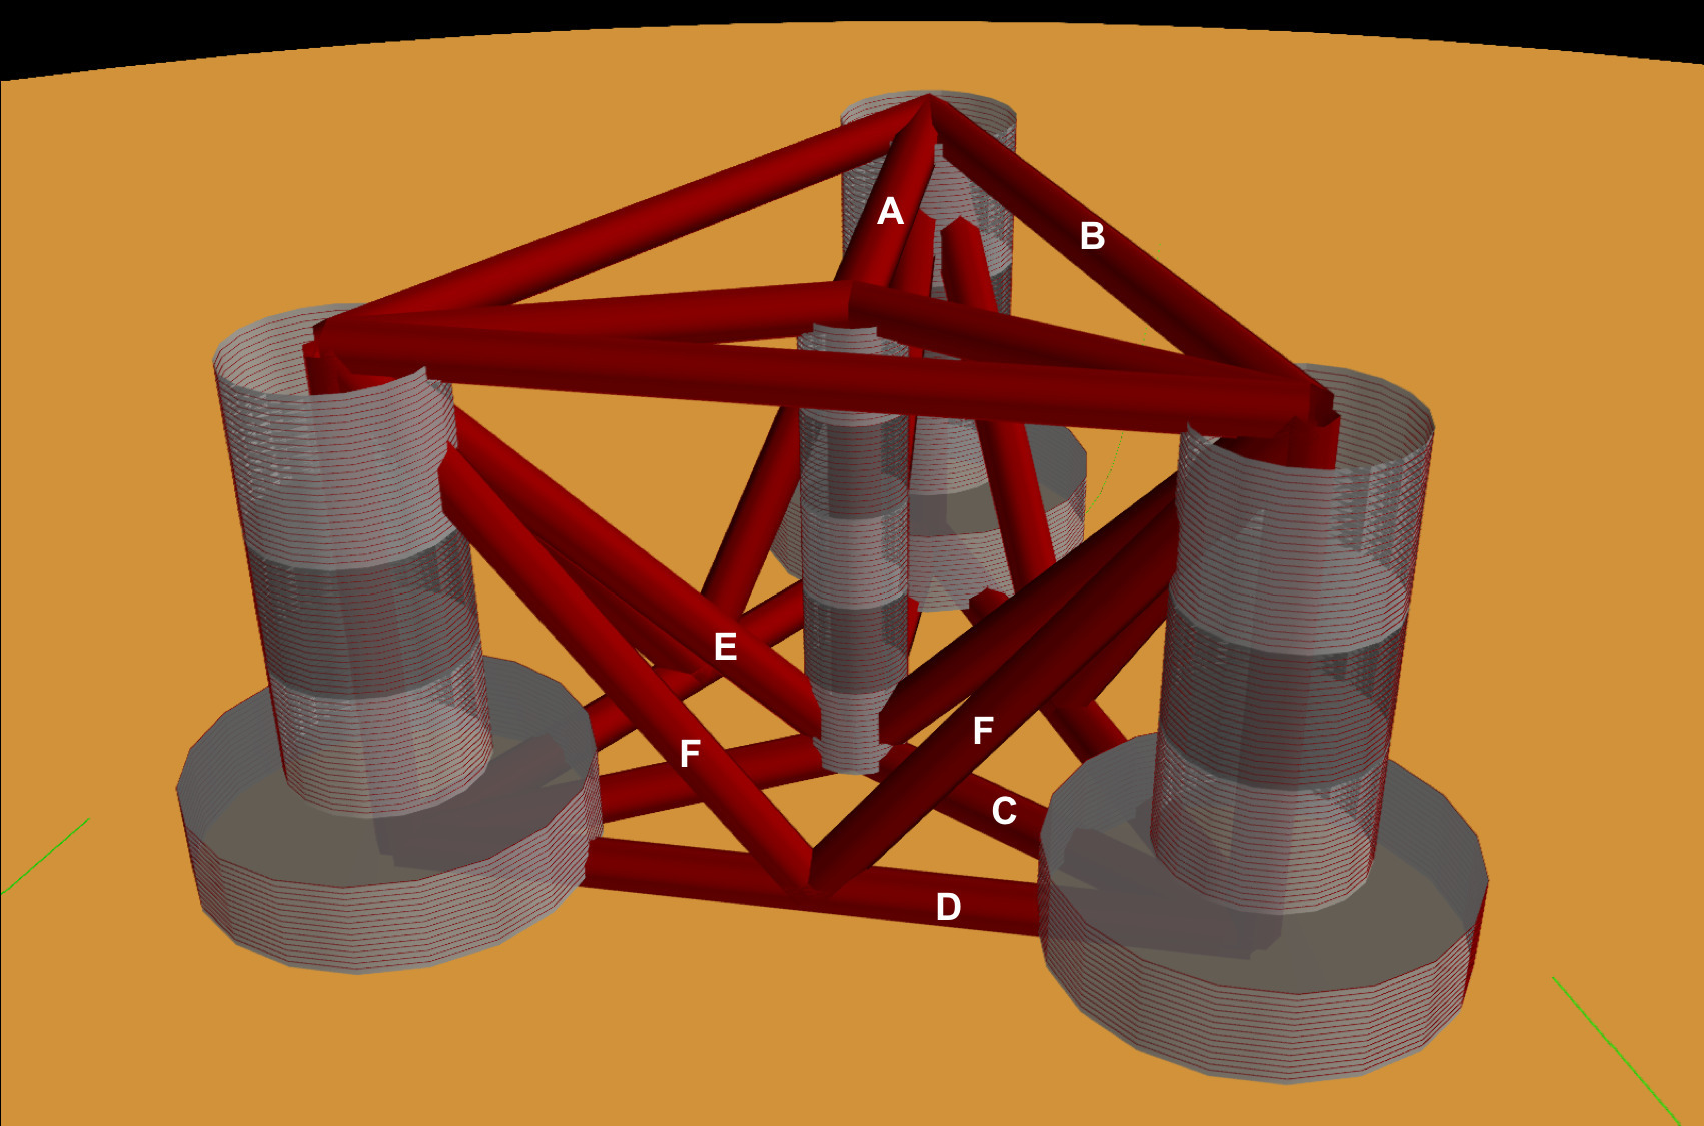
\includegraphics[width=4.5in]{semi}
    \caption{Parameterization of truss elements in substructure.}
    \label{fig:pontoon}
  \end{center}
\end{figure}


\section{Mooring Lines}
The mooring system is described by the number of lines, their geometry,
and their interface to the substructure.  The mooring diameter is set by
the user and determines the breaking load and stiffness of the chain,
via correlation, described in Section \ref{sec:theory}.  The mooring
lines attach to the substructure at the \textit{fairlead} distance below
the water plane, as shown in Figure \ref{fig:diagram}.  The lines can
attach directly to a substructure column or at a some offset from the
outer shell.  Note that bridle connections are not yet implemented in
the model.  The mooring lines attach to the sea floor at a variable
distance, the anchor radius, from the substructure centerline, also set
by the user.

By default, the mooring system is assumed to use a steel chain with drag
embedment anchors. Other mooring available for selection are nylon,
polyester, steel wire rope (IWRC) and fiber-core wire rope.  The only
alternative anchor type is currently suction pile anchors, but there are
plans to include gravity anchors as well.  The standard configuration
for TLPs is the use of taut nylon mooring lines with suction-pile
anchors.

\section{Mass and Cost Scaling}
The mass of all components in the modeled substructure is captured
through calculation of each components' volume and multiplying by its material
density.  This applies to the frustum shells, the ring stiffeners, the
permanent ballast, the pontoons, and the mooring lines.
However, the model also acknowledges that the modeled substructure is
merely an approximation of an actual substructure and various secondary
elements are not captured.  These include ladders, walkways, handles,
finishing, paint, wiring, etc.  To account for these features en masse,
multipliers of component masses are offered as parameters for the user
as well.  Capital cost for all substructure components except the
mooring system is assumed to be a linear scaling of the components
masses.  For the mooring system, cost is dependent on the tension
carrying capacity of the line, which itself is an empirical function of
the diameter.  Default values for all mass and cost scaling factors are
found in Table \ref{tbl:factors}.  Cost factors are especially difficult to
estimate given the proprietary nature of commercial cost data, so
cost rates and estimates should be considered notional.

\begin{table}[htbp]
  \begin{center}
    {\small
      \caption{Default mass scaling factors and cost rates used in
        \textit{FloatingSE} (notional).}
      \label{tbl:factors}
      \begin{tabular}{llcll}
        \textbf{Mass factor} & \textbf{Value} && \textbf{Cost rate} & \textbf{Value} \\
        \hline \hline
        Bulkhead, stiffener & 1.0 && Ballast & \unit[100]{USD/kg} \\
        Column outfitting & 1.06 && Column outfitting & \unit[6,980]{USD/kg} \\
        Tapered column & 1.05 && Tapered column & \unit[4,720]{USD/kg} \\
        Tower outfitting & 1.07 && Pontoons & \unit[6.5]{USD/kg} \\
        \hline
      \end{tabular}
    }
  \end{center}
\end{table}

\section{Design Evaluation}
\label{sec:theory}

\subsection{Design Load Cases (DLCs)}
The user must specify the metocean conditions that drive the wind and
wave loads upon the floating substructure.  \textit{FloatingSE}
currently only uses the single load case of maximum thrust coincident
with maximum wave loading to drive the substructure design. Ideally,
multiple DLCs and metocean conditions would be used for design
optimization.  The capability to optimize over multiple DLCs will be
added to future versions of the model.

\subsection{Load Path}
As with other WISDEM models, the primary simplification in
\textit{FloatingSE} is the treatment of all loads as pseudo-static. This
approximation reduces computational time and resources, since an
accurate calculation of dynamic loads requires more sophisticated
numerical tools and simulations.  Thus, users must exercise care in
selecting loads and safety factors to compensate for the lack of a fully
dynamic treatment \citep{damiani2016}.  Furthermore, fatigue effects and
structural lifetime estimates are also excluded for now, but could be
incorporated in future developments.

A floating wind turbine undergoes loading from a number of sources.  The
primary loading source for the tower comes from the aerodynamic loads
induced by the rotor. The substructure must resist the combination of
both rotor loads and hydrodynamics loads, with the latter becoming more
and more important as water depth and wave heights increase.
\textit{FloatingSE}, together with other WISDEM modules, accounts for
these two dominant load sources, as well as the self-loading of gravity
loads.  Other sources of loading, such as installation loads, accidental
loads, vortex-induced vibrations, ice, and seismic loads are ignored.

\subsubsection{Wind and Wave Loads}
Wind drag loads are applied to the tower body and the upper part of the
substructure that extends above the waterline.  They are not applied to
connecting truss members that may be part of the substructure geometry.
These drag loads are computed assuming the tower and columns are smooth
circular cross-sections and that the drag coefficient can be selected as
a function of the flow Reynolds number \citep{Roshko}.  The drag force
is a function height, since the wind profile and cross-sectional geometry varies
along that dimension.  For the wind profile, the standard power-law
scaling is used,
\begin{equation}
  U_a(z) = U_{ref}\left(\frac{z}{z_{ref}}\right)^{\alpha}\quad,
\end{equation}
where $U_a(z)$ is the wind velocity as a function of height, $U_{ref}$ is a
reference wind speed measured at a reference height, $z_{ref}$, and
$\alpha$ is the shear exponent used in the power-law approximation of
wind profiles.  The wind profile then feeds the aerodynamic drag,
Reynolds number, and drag coefficient,
\begin{equation} \label{eqn:drag}
  dF(z) = \frac{1}{2} \rho_a U_a^2(z) d(z) c_d(Re) dz;\qquad
  Re_d = \frac{\rho_a U_a(z) d(z)}{\mu_a}\quad,
\end{equation}
where $Re_d$ is the Reynolds number based on diameter, $\rho_a$ and
$\mu_a$ are the density and viscosity of air, $d(z)$ is the diameter of
the column as a function of height, $c_d$ is the 2-D drag coefficient, and
$dF(z)$ is the force per unit length in the z-direction.

Wave drag loads arise from similar processes, but are computed using
Morison's equation, a semi-empirical expression that predicts the total
hydrodynamic loads.  It is comprised of two components, one for viscous
drag contributions and another for inertial effects (which includes
incident, diffracted, and radiated wave effects).  For flow past
structures with circular cross sections, Morison's equation for force
per unit length ($dF(z)$) takes the form,
\begin{equation} \label{eqn:morison}
  dF(z) = \frac{\pi d^2(z)}{4} \rho_w C_m \dot{U}_w(z)dz + \frac{1}{2} \rho_w U_w^2(z) d(z) c_d(Re)dz\quad,
\end{equation}
where $C_m$ is the added mass coefficient (assumed to be $C_m=2$),
$U_w(z)$ is the current speed as a function of height, $\dot{U}_w(z)$ is
the acceleration as a function of height, and the Reynolds number is
computed by substituting in the appropriate properties for water,
\begin{equation}
Re_d = \frac{\rho_w U_w(z) d(z)}{\mu_w}\quad.
\end{equation}

To compute Morison's equation, expressions for local fluid velocity and
acceleration are required.  Wave particle velocity (not the same as the bulk
velocity of the wave) is assumed to follow linear (Airy) wave theory
\begin{equation} \label{eqn:Uwave}
U_w(z) = a\omega\frac{\cosh\left[\kappa\left(z + D \right)\right]}{\sinh\left(\kappa D\right)}\cosh\left(\kappa x -
  \omega t\right);
\qquad \omega=\frac{2\pi}{T} = \sqrt{ g \kappa \tanh\left(\kappa
    D\right) } \quad,
\end{equation}
where $\omega$ is the circular frequency, $T$ is the wave period, $a$ is
the wave amplitude (half of the significant wave height), $D$ is the
total water depth, $g$ is the acceleration of gravity, and $\kappa$ is
the wave number numerically computed from the dispersion relationship
given as the last expression in Equation \ref{eqn:Uwave}.  Note that the
horizontal particle velocity varies in time and space (by the
$\kappa x - \omega t$) term.  Thus, the individual particles in the wave
are also accelerating at different rates,
\begin{equation} \label{eqn:Awave}
\dot{U}_w(z) = a\omega^2\frac{\cosh\left[\kappa\left(z + D \right)\right]}{\sinh\left(\kappa D\right)}\sinh\left(\kappa x -
  \omega t\right)\quad.
\end{equation}
For
simplicity, \textit{FloatingSE} only considers the maximum velocity and
acceleration at a given height, and makes a conservative assumption that
they occur concurrently in time and space.  This essentially means ignoring the
$\kappa x - \omega t$ term, since the maximum of any hyperbolic sine or cosine
term is one.


\subsubsection{Rotor Nacelle Assembly (RNA) Loads}
From a quasi-steady-state point of view, the RNA loads reduce to three
forces and three moments along the main coordinate axes
\citep{JacketSE}. The thrust is the biggest force responsible for the
bending moment distribution along the tower and loads on the
substructure.  There is the additional effect of the gravitational load
caused by the offset of the RNA center of mass from the tower
centerline.  This effect is more pronounced for downwind turbines than
upwind turbines, but is included regardless.  \textit{FloatingSE} does
not compute the force and moment components directly, but rather accepts
them as inputs from other WISDEM modules or from the user directly.


\subsection{Structural Analysis}
The analysis tool, Frame3DD, is an open-source tool for static and
dynamic structural analysis of 2-D and 3-D frames and trusses with
elastic and geometric stiffness. It computes the static deflections,
reactions, internal element forces, natural frequencies, and modal
shapes using direct stiffness and mass assembly \citep{frame3dd}.  The
WISDEM toolkit developed a python interface, \textit{pyFrame3DD}, to
avoid the use of intermediate input and output text files.  The
integration of all loads happens within Frame3DD, where the whole floating
turbine load path, from the rotor to the keel of the substructure, is
modeled with Timoshenko frame elements \citep{timoshenko}.

\subsubsection{Discretization}
For the finite element structural analysis of the substructure, the
discretization of the main columns into a handful of sections is still
too coarse to capture the appropriate physics. Long slender components,
such as the tower and substructure columns, are broken up into a
three-times finer discretization than the physical cans that they are
actually made of.  The sectional and nodal variables are re-sampled at
this finer spacing.  These additional discretization points give greater
resolution of internal forces and natural frequencies.  Substructure
pontoons are represented as single frame elements.  Frame elements are
described by their cross sectional properties (area, moments of inertia,
modulus of elasticity, and mass density) and starting and ending nodes.
For simple geometries, such as pontoons with tubular cross sections,
these properties are straightforward calculations.  For the turbine
tower, tubular cross section properties are also used, albeit at a finer
discretization.  For substructure columns, it is assumed that the
permanent or variable ballast and bulkheads are not load-bearing, so
tubular cross section properties are also used to represent the column
shell.  However, the material mass density of the frame element is
scaled to reflect the true mass of the whole section, including ballast,
to ensure that gravity loads are captured correctly.

\subsubsection{Loads}
All of the loads described above are integrated together within
Frame3DD.  These loads include,
\begin{itemize}
\item Rotor-nacelle-assembly loads (thrust, moments, etc)
\item Mooring line force
\item Wind and wave loading
\item Gravity loads (weight distribution)
\item Hydrostatic pressure loads, including buoyancy
\end{itemize}

The forces, moments, and mass properties of the rotor-nacelle assembly
(RNA) are inputs to \textit{FloatingSE} (mass properties are assumed to
be relative to the tower top position).  It assumed that the RNA is a
rigid body with respect to the tower modes and the mass properties,
forces, and moments, are applied to the corresponding node in the model.
The forces along each mooring line are applied to the connection
point nodes on the structure.  The wind and wave forces per unit length
in Equations \ref{eqn:drag} and \ref{eqn:morison} are applied as
trapezoidally varying loads along the column elements.  Other loads
applied to the structure include the gravity loads, and the buoyancy
acting on the submerged elements.

\subsubsection{Boundary Conditions}
Multiple boundary conditions are applied to the structure.  The mooring
system stiffness matrix (linearized about the neutral position) is
applied at the mooring connection nodes.  However, even with the mooring
stiffness, the finite element analysis would otherwise still regard the
structure as unrestrained and incapable of supporting any static loads.
Thus, in order to successfully compute stress and buckling limits in a
well-posed problem, an additional rigid boundary condition (in all 6
DOF) is imposed at the bottom node of the main column.

\subsubsection{Outputs}
Structural analysis outputs include mass properties of the structure,
member stresses, and summary forces and moments on the body.  Mass
properties include the total mass of the floating turbine and the mass
of the substructure itself.  The calculations also allow for easy
computation of the center of mass of the structure (not accounting for
variable ballast) and the center of buoyancy (centroid of the submerged
volume).  The first two natural frequencies of the structure are also
computed to compare against the range of standard wave frequencies and
rotor passing frequencies (1P and 3P).  Next, the reaction forces and
moments at the boundary node at the keel are taken as the total loading
on the structure.  These are used later in the static stability
calculations to ensure that the mooring lines provide adequate restoring
force and moment.  Finally, the axial and shear forces within each frame
element are extracted and converted to stresses using cross-sectional
properties.

Hoop stress of the tower is estimated from the dynamic pressure of the
wind loads using the Eurocode method \citep{Eurocode}.  Hoop stress of the submerged
columns is determined using the dynamic and static pressure heads of the
water.
\begin{align}
  \sigma_{\theta,Euro} &= k_w q_{max} \frac{d-t}{2t};\qquad q_{max} =
                         \frac{1}{2}\rho_a U_a^2\\
  \sigma_{\theta,hydro} &= \left(q_{max}+p_{hydro}\right) \frac{d-t}{2t};\qquad q_{max} =
                          \frac{1}{2}\rho_w U_w^2\\
  p_{hydro} &= \rho_w g \left( a\frac{\cosh\left[\kappa\left(z + D \right)\right]}{\cosh\left(\kappa D\right)} - z\right)
\end{align}
where $\sigma_{\theta}$ is the hoop stress, $q_{max}$ is the maximum
dynamic pressure on a cross-section, and $p_{hydro}$ is the hydrostatic
pressure with contributions from wave motion and the static head.  In
the Eurocode method, $k_w$ is the dynamic pressure factor for hoop
stress calculation using cylinder dimensions and an external pressure
buckling factor.  Note that the argument, $(z)$, was dropped from many
of the terms without losing generality.



\subsubsection{Code Compliance as Utilizations}
Once the stress components of all structural members are computed, they
are compared against design code standards for compliance, and serve as
design constraints when conducting optimization.  Multiple code
standards are used across all components.  For all columns, the tower,
and substructure pontoons, stress components (axial, shear, and hoop)
are combined into a von Mises, equivalent, stress,
\begin{equation}
  \sigma_{vm} = \sqrt{\sigma_a^2 + \sigma_{\theta}^2 -
    \sigma_a\sigma_{\theta} + 3\tau_{a\theta}^2}
\end{equation}
where $\sigma_{vm}$ is the von Mises stress, $\sigma_a$ is the axial
stress, $\tau_{a\theta}$ is the shear stress across axial and hoop
principle directions.  and $\sigma_{\theta}$ is chosen as the relevant
hoop stress.  The von Mises stress is compared against the yield stress,
$\sigma_y$, and a safety factor as a utilization criterion.

Main column, offset column, and tower segment stresses and geometry are
also evaluated against a shell buckling criterion published by
\citet{Eurocode} and a global buckling criterion published by
\citet{Germanischer}.  Note that the implementation of the Eurocode
buckling is modified slightly so as to produce continuously
differentiable output.  See \citet{JacketSE} for a more detailed
exposition.

For submerged columns, additional code standard utilization ratios are
taken from the \citet{api2U}, Bulletin 2U (specifically the procedure
outlined in Appendix B).  These standards also apply shell and general
buckling criterion with a margin of safety in a manner that accounts for
stiffeners and the common buckling modes of submerged structures.
Future efforts will also apply Bulletin 2V, the standards for plates, to
the legs that support taut mooring lines.


\subsection{Mooring Lines}
The quasi-steady mooring system analysis is handled by the external
Mooring Analysis Program (MAP++) library \citep{MAP}, which has
convenient Python bindings to access the simulation output, bundled into
the WISDEM \textit{pyMAP} module. MAP++ is designed to model the
steady-state forces on a Multi-Segmented, Quasi-Static (MSQS) mooring
line. Seabed contact, seabed friction, and multi-element mooring lines
with arbitrary connection configurations can be analyzed.  MAP++ inputs
include sea depth, geometry descriptions of the mooring line
connections, and material properties of the lines.  For chain and
rope-based cables, these material properties are not easily derived and
would be typically provided by a manufacturer.  We borrow from the
approach of the popular Orcina OrcaFlex software \citep{orca} and use
the following expressions,
\begin{align*}
MBL &= 2.74\times 10^7  d^2 \left(44 - 80d\right) \,[\unit{N}] \\
mass &= 19.9\times 10^3 d^2 \,[\unit{kg/m}]\\
A &= 2\left(\pi d^2 / 4 \right)\,[\unit{m^2}]\\
EA &= 8.54\times 10^{10} d^2\,[\unit{N}]\\
cost &= 3.415\times 10^4 d^2 \,[\unit{USD}]
\end{align*}
where $MBL$ is minimum breaking load, $d$ is the diameter of a single
half-chain link, $A$ is the chain cross-sectional area, $E$ is the
Young's modulus, $EA$ is the axial stiffness.  When conducting
optimization, the expression for $MBL$ is poorly posed due to its limited
range of diameter applicability, so a linear fit is used instead,
\begin{equation}
MBL = 1000 \max\left(1.0, -5445.3 + 176972.7 d\right)
\end{equation}  


\subsection{Hydrostatic Stability}
\label{sec:static}
\subsubsection{Neutral Buoyancy}
Any floating body requires enough water displacement to create
sufficient buoyancy force such that the body stays afloat in the most
extreme loading and environmental conditions.  This level of
displacement would otherwise be overkill for more benign loading
conditions.  Since a floating turbine is designed for a constant hub
height, variable amounts of ballast are required to maintain a neutrally
buoyant system for all operating conditions.  The variable ballast is
simply ocean water that is pulled in or pumped out of holding areas
within the substructure columns.

In \textit{FloatingSE}, the variable ballast water mass is calculated as
the difference between the total mass of displaced water and the total
mass of the floating turbine.  This mass is then divided by the water
density to obtain the variable ballast volume, which is then compared to
the frustum shell cross section profile above the permanent ballast to
determine the height of the water ballast within the column.  Once this
is determined, the final center of mass of the system can be determined.

\subsubsection{Surge/Sway Stability}
Surge and sway stability is not actively tracked over the coarse of a
load case.  Instead the total surge force on the structure is calculated
at the initial conditions and compared to the restoring force of the
mooring system at the maximum allowable surge offset, which is specified
by the user.

The surge direction is assumed to be aligned with the wind vector, which
is aligned with the $x$-axis.  Since the rotor yaw is assumed to be
$0^{\circ}$, the surge forces on the turbine include the rotor thrust
and the wind and wave drag on the tower and substructure.  The final
surge force over the whole structure is taken from the $x$-direction
reaction force of the reaction node in Frame3DD.

The restoring force is calculated as the smallest possible restoring
force after a displacement in any angular direction in the mooring
model.  Since the alignment of the mooring lines relative to the
incoming wind direction is arbitrary, a maximum offset is simulated at
$2^{\circ}$ increments around the unit circle. Also recorded in this
survey is the maximum mooring line tension in any
line, in any direction, for comparison against the minimum breaking load
value,
\begin{equation}
  F_{x,restore} = \min_{i\in a} F_{x,i}\quad \mbb{T}_{moor} = \max_{l\in L,i\in a} \mbb{T}_{l,i}\,;
\qquad L=\left\{1,2\ldots nlines\right\}, \, a= \left\{0^{\circ}, 2^{\circ}\ldots 360^{\circ}\right\}
\end{equation}
where $F_x$ is the surge force and $\mbb{T}$ is the tension.  If
restoring force at this maximum offset is greater than the surge force
applied, then the system is considered stable in surge.  Since the wind
and wave profiles are essentially 2-D in the $x-z$ plane, the sway
stability is given the same status as surge stability.


\subsubsection{Pitch Stability}
The approach to pitch stability determination is similar to that of
surge stability.  The total pitching moment on the floating turbine is
calculated and compared to the restoring moment at the maximum allowable
angle of heel.  If the restoring moment at this max heel angle is
greater than the pitching moment applied, the system is said to be
statically stable in pitch.

Similar to the surge force calculation, the total pitching moment is
determined from the reaction moment at the boundary condition
in the Frame3DD analysis.  The pitching moment has contributions from
the wind and wave loads on the structure, the rotor forces and torques,
the buoyancy forces on the submerged substructure, and the off-center
weight of components (e.g. the RNA).

The restoring pitching moment has two primary contributions.  The first
is from the mooring lines.  Similar to the surge force calculation, here
the floating turbine is deflected in pitch by the maximum allowable heel
angle and the mooring forces are recorded.  The restoring moment
contribution from the mooring system is computed as,
\begin{equation}
  \mbf{M_{moor}} = \sum_i \mbf{r_{cm-l}} \times \mbf{F_l}
\end{equation}
where $r_{cm-l}$ is the vector from the center of mass to the mooring
connection, and $F_l$ is the force applied by the $l$-\th\~mooring
line.  As above, $F_l$ is taken as the minimum set over the possible
orientations of the mooring lines relative to the direction.

\begin{figure}[htb]
  \begin{subfigure}[b]{0.49\linewidth}
    \centering 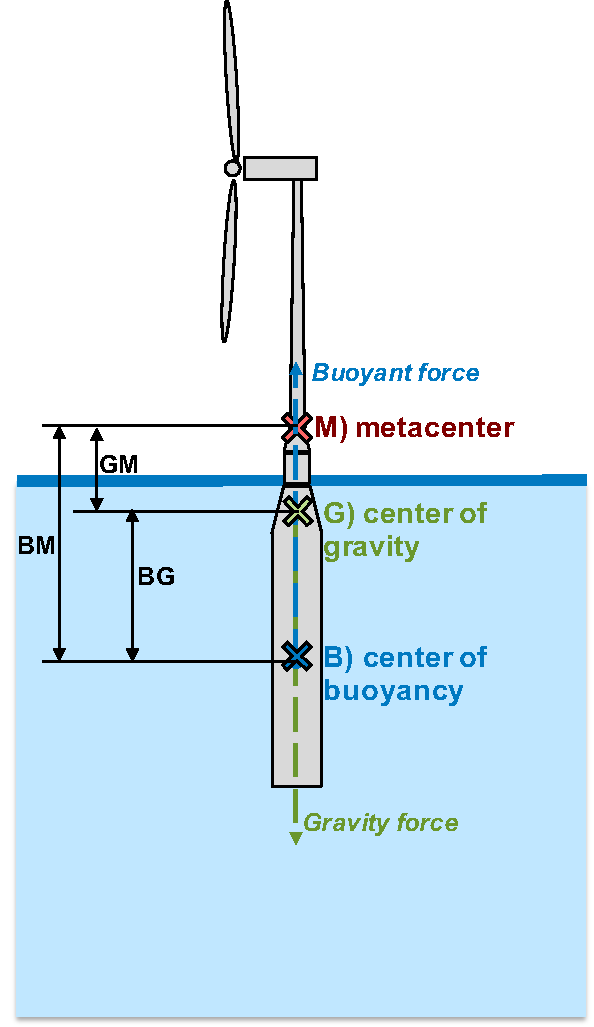
\includegraphics[height=3.5in]{figs/metacenterA.pdf}
    \caption{}
  \end{subfigure}
  \begin{subfigure}[b]{0.49\linewidth}
    \centering 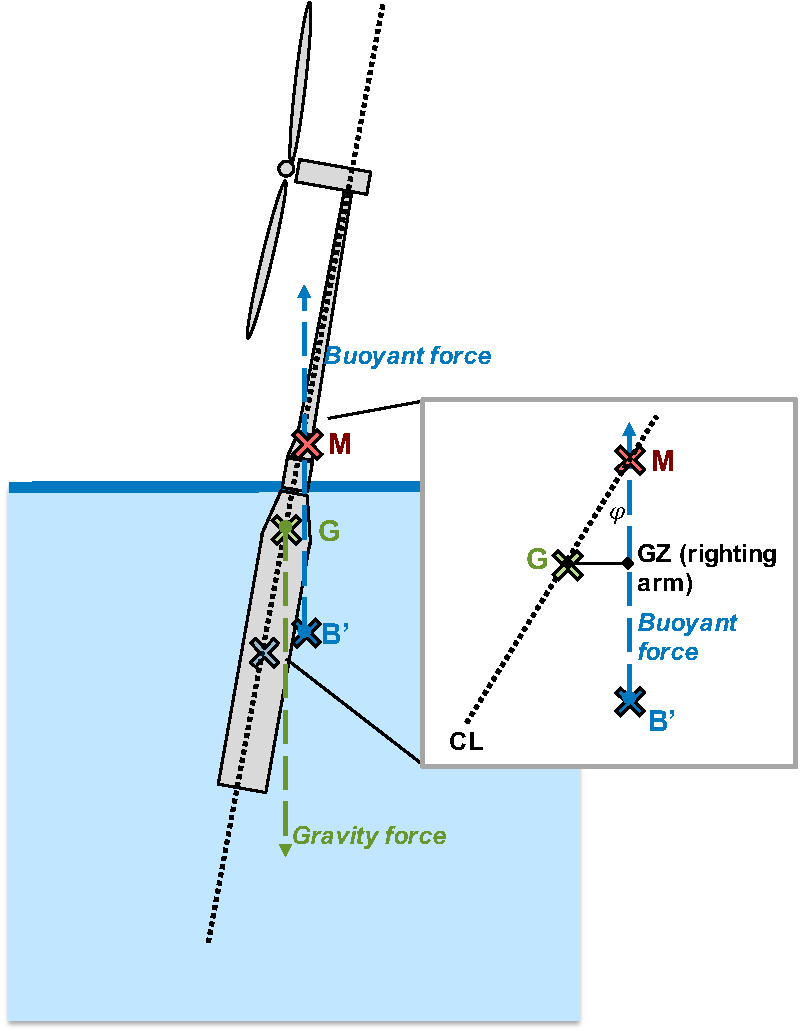
\includegraphics[height=3.5in]{figs/metacenterB.pdf}
    \caption{}
  \end{subfigure}\\
  \caption{Static stability of floating offshore wind turbines.}
  \label{fig:metacenter}
\end{figure}

The second contributing restoring moment comes from the motion of the
center of buoyancy away from alignment with the center of mass.  This is
a standard calculation in naval architecture \citep{thiagarajan2014} and is
diagrammed in Figure \ref{fig:metacenter}.  In this diagram, the center
of mass is denoted, $G$, the center of buoyancy is $B$, and the
metacenter is $M$.  In neural conditions (Figure \ref{fig:metacenter}a),
all of these points are vertically aligned.

As the structure lists or heels, the center of buoyancy shifts toward
the side of the structure that is more submerged (from $B$ to $B'$) and
the buoyancy force no longer passes through the center of mass.
Instead, the buoyancy force passes through the metacenter with an
effective moment arm of $GZ$ from the center of mass (Figure
\ref{fig:metacenter}b).  The metacenter is defined as the common point
through which the buoyancy force acts as it pitches through small
displacements, for bodies with sufficient freeboard margin.

The metacenteric height, $GM$ is most easily calculated as an offset from the
center of buoyancy ($BM$) by,
\begin{equation}
  h_{meta} = M - G = GM = BM + BG;\quad BM = \frac{I_w}{V}
\end{equation}
where $BG$, the distance between the centers of buoyancy and gravity is
easily calculated, $I_w$ is the second moment of area of the substructure waterplane
(with units of \unit{$m^4$}) and $V$ is the total volume of displacement
(with units of \unit{$m^3$}).  Note that for semisubmersible type
geometries, $I_w$ is calculated with the parallel axis theorem for all
of the columns at the waterplane,
\begin{equation}
  I_w = \sum_i \left( I_{w,i} + S_ir_i^2 \right)
\end{equation}
where $S_i$ is the waterplane cross sectional area of the $i$-\th column and $r_i$
is the distance from the waterplane centroid to the $i$-\th column centroid.

The restoring moment is then the buoyancy force acting through the
restoring arm, $GZ$,
\begin{equation}
  M_{meta} = F_B GZ = F_B GM \sin \varphi
\end{equation}
where $\varphi$ is the angle of heel.

For this reason, the metacenter must be located above the center of mass
for static stability.  This condition is imposed on the design as a
constraint.  Note that the total volume of displacement, and the
subsequent buoyancy force, is not recalculated in the perturbed
configuration.  It is assumed that the angles of deflection are small
and that there is sufficient freeboard and design symmetry such that the
total displacement is constant.

The total restoring pitching moment is then the sum of two
contributions,
\begin{equation}
  M_{y,restore} = M_{y,moor} + M_{meta}
\end{equation}

\subsection{Hydrodynamic Stability}
Floating bodies are typically modeled, for small motions and linearized
behavior, as a second-order differential system with mass, damping, and
spring stiffness terms,
\begin{equation}
  \left(\mbf{M} + \mbf{A}\right)\ddot{\mbf{x}} + \mbf{C}\dot{\mbf{x}} +
  \mbf{K} = \mbf{F}\left( t \right)
\end{equation}
where $\mbf{x}\in\mbb{R}^6$ is the six-degree of freedom vector
(commonly ordered as 1-surge, 2-sway, 3-heave, 4-roll, 5-pitch,
6-yaw), $\mbf{M}$ is the mass matrix, $\mbf{A}$ is the added mass
matrix, $\mbf{C}$ is the damping matrix, and $\mbf{K}$ is the stiffness
matrix.  The right-hand side of the equation captures the time-dependent
summation of all forces.

As a low-fidelity, quasi-static sizing and cost module,
\textit{FloatingSE} does not attempt to capture all of the matrix
entries or forcing terms of the hydrodynamics.  A more sophisticated
time- or frequency-domain solver, where these quantities are calculated,
may be linked or included into \textit{FloatingSE} in the future.
Nevertheless, it does attempt to compute the diagonal entries of the
mass and stiffness matrices in order to derive the rigid body natural
frequencies of the system,
\begin{equation}
  f_i = \frac{\omega_i}{2\pi} =
  \frac{1}{2\pi}\sqrt{\frac{K_{ii}}{M_{ii}+A_{ii}}}, \quad \forall i \in
  \left[1\ldots6\right]
\end{equation}
where $f_i$ are the frequencies of the eigenmodes and $\omega_i$ is the
circular frequency.  The mass matrix diagonal entries, $M_{ii}$, are simply the mass and
moments of inertia of the whole system,
\begin{equation}
  M_{11} = M_{22} = M_{33} = m_{sys};\quad M_{44} = I_{xx,sys};\quad M_{55} = I_{yy,sys};\quad M_{66} = I_{zz,sys};
\end{equation}
Where the coordinate system notation is consistent with that of Figure
\ref{fig:diagram}.

The added mass matrix diagonal entries are evaluated via standard strip
theory for the tapered vertical columns.  The added mass for the system is a
summation over the columns, using the parallel axis theorem for the
rotational degrees of freedom.  Pontoon contributions to system added
mass are currently ignored.  The column quantities are calculated as,
\begin{equation}
  A_{11} = A_{22} = \rho V;\quad A_{33} = 
  \left(\frac{1}{2}\right)\frac{8}{3} \rho \max \left[ R^3(z)\right] ; \quad A_{44} =
  A_{55} = \pi\rho\int\left(z-z_{cb}\right)R^2(z)dz;\quad A_{66} = 0.0;
\end{equation}
where $\rho$ is the water density, $R(z)$ is the column radius along its
axis, and $V$ is the submerged volume.  The extra factor of $1/2$ in
$A_{33}$ is included to account for the fact that the top of the column
extends above the waterline.  Also, the integral in $A_{55}$ is only evaluated
along the submerged portion of the column.

The stiffness matrix is comprised of contributions from the mooring
and hydrostatic stiffness.  The mooring linearized stiffness matrix is output
directly from MAP++ and needs no additional processing within
\textit{FloatingSE}.  The hydrostatic stiffness, for a vertical column, is derived from the same
principals described above regarding the metacentric height,
\begin{equation}
  K_{ii} = K_{ii}^{moor} + K_{ii}^{hydro};\quad K_{33}^{hydro} = \rho g
  S_{sys};\quad K_{44}^{hydro} =  K_{55}^{hydro} = \rho g V h_{meta}
\end{equation}
where $S_{sys}$ is the waterplane area of the system.

Once the rigid body natural frequencies (eigenmodes) of the system are
calculated, they are compared against the standard wave frequencies
range, \unit[0.5--5]{Hz}, and expressed as a design constraint (with a
partial safety factor).


\subsection{Validation}
The International Energy Agency has sponsored a number of international
research collaborations to further the state of wind energy technology and
tools.  One of these, Task 30: Offshore Code Comparison Collaboration
(OC3), shared a spar design among many participants to compare
performance as modeled by differed tool sets.  A description of the OC3
spar is provided in \citet{OC3}.  Since it is already a
well-studied geometry, this design was selected as the focus of
verification for \textit{FloatingSE}.  As part of the Task 30 effort,
an ANSYS model of the OC3 spar, using shell elements combined with
stiffeners and bulkheads, was also generated.  This was taken as
the \textit{truth} standard for comparison.

The first step in the verification exercise was to ensure that the mass
properties of the spar predicted by \textit{FloatingSE} matched those
calculated by ANSYS.  The comparison showed that the \textit{FloatingSE}
summary mass estimates are within $1\%$ error of ANSYS.  The second step
was a comparison of static loading stresses.  The spar was simulated in
quiescent air and water (no wind, waves, or current), which isolated the
weight of the turbine and hydrostatic pressure forces as the only load
sources on the substructure.  The effective von Mises stress, as
calculated by \textit{FloatingSE}, was compared to the ANSYS model.  The
\textit{FloatingSE} stress calculation matches that of ANSYS nearly
exactly over the top half of the spar, but deviates by approximately
5--10\% towards the bottom half of the spar.  In the bottom half of the
spar, \textit{FloatingSE} actually over-predicts the stress, a more
conservative estimate, which is the preferable approach in a
low-fidelity cost and sizing model.  At this time, more complicated
loading cases, with wind and wave loading included, have not been
performed.

The rigid body modes predicted by \textit{FloatingSE} were compared
against a FAST model of the OC3 spar.  FAST was used as the truth
solution in this case because it more accurately handles mooring
dynamics than the ANSYS structural model and more accurately captures
hydrodynamic phenomenon.  The errors in the surge, sway, roll, and pitch
frequencies are 11-12\%.  \textit{FloatingSE} actually estimates the
heave mode frequency quite accurately, to less than 1\% error, but is
significantly off in estimating the yaw mode frequency.  This was deemed
acceptable as there is no focus on the yaw DOF in \textit{FloatingSE}.




\chapter{Analysis}
\label{sec:opt}

\section{Procedure}
Single scenario execution of \textit{FloatingSE} and/or WISDEM is
sufficient to explore some simple one-off or comparison analyses between
a few runs.  However, executing the model within an optimization
framework can give yield richer and more insightful analyses.  There are
two layers of optimization-based analyses presented in this work:

\begin{enumerate}
\item Use \textit{FloatingSE} and WISDEM to design a spar,
  semisubmersible, and TLP floating substructure for the same turbine
  configuration;
\item Conduct a sensitivity analysis around the optimized designs for
  weight reduction at the top of the tower by parametrically changing
  the mass of the nacelle and re-optimizing the substructure.
\end{enumerate}

\subsection{Substructure Design}
The first step in the analysis procedure is the conceptual design of a
spar, semisubmersible, and TLP floating substructure for the same
turbine configuration.  Many studies in the literature focus on the
optimization of a single substructure design.  By showcasing the design
of all three classical substructure archetype, we demonstrate the ability
of the tool to capture a broad tradespace.

Through its various modules, WISDEM is fully capable of optimizing the
entire turbine design, from the rotor through the drivetrain and down
through the tower and substructure.  However, in an effort to focus on
the capabilities of \textit{FloatingSE}, the turbine was held fixed to
the DTU \unit[10]{MW} reference definition throughout the substructure
design and sensitivity analysis.  The only exception being the
deliberate modification of the nacelle mass for the sensitivity study.
This isolated the design variables and constraints to be those
associated with the substructure exclusively.

\subsection{Sensitivity Studies}
Following the successful conceptual design of the floating
substructures, a sensitivity study was executed relating the mass at the top of the
tower to the mass and cost of the substructure.  This was accomplished
by parametrically changing the nacelle mass and re-optimizing the
substructure designs.  Specifically, the nacelle mass was changed from
its nominal value to the perturbations of, $[+10\%, -10\%, -25\%, -33\%,
  -50\%]$.  For the sensitivity study, the re-optimization was done locally,
using the previously optimized designs as a starting point, and not
searching over the global tradespace.  Then, by
comparing the baseline design to the re-optimized designs under the
parameterized mass changes, the cost value of mass savings can be
determined.  Meaning, given the quantified mass and cost removed from
the substructure relative to the baseline design, the cost value of the
mass savings in the nacelle can be quantified.  In this way, a systems
framework can determine with the cost premium for the nacelle mass
reduction can be recovered through savings as the change is propagated
throughout the rest of the system.

The parametric modification of the nacelle mass is not merely an
academic exercise to tease out design sensitivities.  There are many
examples of a new technology or innovation that offers a component mass
reduction at a cost premium.  By parametrically changing the nacelle
mass, the sensitivity study is capturing the implications of moving from a
multi-stage geared drivetrain to a single-stage or direct-drive
alternative, or from a permanent magnet generator to a superconducting
generator.  In both of these examples, the overall mass of the nacelle
would likely decrease, but the new technology would cost more to
implement over the legacy system.  Conducting an honest cost-benefit
tradeoff of this option requires the potential design changes be
propagated through the rest of the system.  WISDEM is an appropriate
framework for posing and answering this type of question.


\subsection{Reference Turbine Selection}
For all elements of the optimization studies, attention is given to the
substructure and the performance of \textit{FloatingSE}.  A reference
turbine design was needed as a starting point by which the conceptual
design and sensitivity studies could build upon.  The Danish Technical
University (DTU) \unit[10]{MW} reference design was chosen as the static
turbine to be used throughout this analysis.  This selection was made
because \unit[10]{MW} is commensurate with the most current offshore
turbine designs being installed (with fixed-bottom supports) by
developers.  Additionally, other research efforts, such as the LIFES50+
program, have already designed floating substructures for this turbine.
Using the same reference turbine allows for a direct comparison of the
designs produced here with the other designs documented in the
literature.  For a summary of the DTU \unit[10]{MW} reference turbine,
see \citet{dtu10mw}.


\subsection{Metocean Conditions}
In addition to choosing a reference turbine, it was also necessary to
choose the meteorological and oceanographic (metocean) conditions of the
environment.  As mentioned in Section \ref{sec:theory},
\textit{FloatingSE} only uses a single DLC, the maximum rotor thrust and
metocean loading, for concept evaluation.  The metocean condition
selected for this DLC is the same as that used in the IEA Wind Task 30
OC3 effort \citep{OC3}, and summarized in Table \ref{tbl:metocean}.

\begin{table}[htbp] \begin{center}
    \caption{Metocean conditions used as the design point in the design
      and sensitivity studies (adopted from \citet{OC3}).}
    \label{tbl:metocean}
          {\small
            \begin{tabular}{ l l } \hline
              \textbf{Parameter} & \textbf{Value} \\ \hline \hline
              Wind reference speed & \unit[11]{$m/s$} \\
              Wind reference height & \unit[119]{$m$} \\
              Water depth & \unit[320]{$m$} \\
              Significant wave height & \unit[10.8]{$m$} \\
              Significant wave period & \unit[9.8]{$s$} \\ \hline
            \end{tabular}
          }
\end{center} \end{table}


\section{Methodology}
In this project, optimization studies start with the formulation of
a constrained, nonlinear single-objective optimization problem with
mixed-integer design variables,
\begin{equation}
\begin{array}{ll}
  \min & f\left(\mbf{x}\right)\\
  \text{subject to} & \mbf{g}\left(\mbf{x}\right) \leq 0,\\
  \text{and}& \mbf{x} \in \mbf{X} \\
  \end{array}
\end{equation}
where,
\begin{itemize}
\item $\mbf{x}$ is a vector of $n$ \textit{design variables}, the variables that are adjusted in order to
  find the optimal solution (see Table \ref{tbl:designvar});
\item $f(\mbf{x})$ is the nonlinear \textit{objective function}, the
  metric to be minimized by the optimization algorithm;
\item $\mbf{g} (\mbf{x})$ is the vector of \textit{inequality constraints}, the
  set of conditions that the solution must satisfy (see Table
  \ref{tbl:constraints}).  There are no equality constraints;
\item $\mbf{X}$ is the design variable \textit{bounds}, the bracket of
  allowable design variable values.
\end{itemize}

Note that this problem statement imposes no requirements on the types of
variables in $\mbf{x}$.  A mixed-integer solution is desired, where some
design variables are continuous ($x \in \mbb{R}$) and others are
discrete variables that can only take integer values ($x \in
\mbb{Z}$).  An example of an integer design variable in this
application is the number of offset columns or the number of mooring
line connections.


\subsection{Objectives}
As described above, two objective functions are used in this analysis:
\begin{itemize}
\item \textbf{Substructure system mass:} The mass of components from the
  freeboard point and below \textit{except} mooring and anchor system masses;
\item \textbf{Substructure system cost:} The capital cost of components from the
  freeboard point and below \textit{including} mooring and anchor system costs;
\end{itemize}


\subsection{Algorithms}
Two derivative-free optimization algorithms were applied sequentially to
the substructure design problem:
\begin{enumerate}
\item \textbf{Global design space search and optimization:} Native
  implementation of the Non Sorting Genetic Algorithm (NSGA)-II genetic
  algorithm \citep{nsga2} with some modifications for constraint and
  integer design variable handling;
\item \textbf{Local neighborhood design space optimization:} Native
  implementation of the Nelder-Mead simplex algorithm \citep{neldermead}  with some
  modifications for constraint handling.
\end{enumerate}

The global design space search was performed by a modified
implementation of the popular NSGA-II \citep{nsga2} algorithm.  This algorithm is
a non-dominating sorting genetic algorithm that solves non-convex and
non-smooth single and multiobjective optimization problems. The
algorithm attempts to perform global optimization, while enforcing
constraints, using a tournament selection-based strategy where the best
solutions are placed into a mating pool.  The local modifications of the
NSGA-II algorithm include parallelization via multi-threading for faster
execution, the use of penalties for constraint handling (described
below), and the handling of integer-based design variables for a fully
mixed-integer capable solution.  Specifically, a method for
integer-coded design variable crossover and mutation, standard genetic
algorithm operations, were developed.  Crossover of an integer design
variable across two population members with integer values $z_1$ and
$z_2$ is simply a random integer in the interval, $[z_1, z_2]$.
Similarly, mutation of an integer design variable is a random integer
number selected between the lower and upper bounds.

The user selected parameters and initial conditions for the NSGA-II
algorithm were selected to foster a broad and fluid search of the entire
tradespace.  A population size of 30 was initialized with Latin
Hypercube sampling across the range of permissible design variable
values from the lower bound to the upper bound.  Thus, this was truly a
\textit{tabula rasa} (blank slate) approach to substructure design.  The
probability of crossover during the optimization was set to 0.9 and the
probably of mutation was 0.4.  Both of these values are considered high,
in the context of genetic algorithm scientific literature, but again
enabled a broard and fluid search of the tradespace.

By design, the NSGA-II algorithm is well-suited to global optimization
by traversing a broad span and combination of design variable values.
However, for single-objective optimization (such as mass or cost
minimization), the crossover and mutation operations, with their
inherent use of random numbers, are inefficient at searching a design
space neighborhood for local minima.  Thus, after the genetic algorithm
terminated, another local optimization was performed.

Local optimization was performed with the Nelder-Mead simplex algorithm
\citep{neldermead}.  The Nelder–Mead method, also referred to as the
downhill simplex method, is a derivative-free heuristic optimization
method.  It uses a simplex, a shape with $n+1$ vertices in
$n$-dimensional space (e.g. a triangle on a plane or a tetrahedron is
three-dimensional space), to approximate the objective function
behavior.  The vertices of the simplex, the test points, are then
reflected, expanded, or contracted to move towards the optimal point.
The process terminates when the simplex becomes sufficiently small or
the test points have nearly identical performance.  As with the genetic
algorithm, a local implementation of the Nelder-Mead algorithm was used
to enable multi-threading and constraint handling via the chosen penalty
method.  To focus the algorithm purely on local optimization, and not
global exploration of other possible floating substructure
configurations, only continuous design variables were used.  Integer
design variables such as the number of offset columns or mooring lines
were frozen at their values chosen by the NSGA-II algorithm.
Additionally, since this approach is best suited for finding local
minima near the initial condition, it is the only algorithm used for the
design sensitivity portions of the analysis.

User parameters values and simplex initialization methodology was
borrowed from the open source SciPy implementation of the Nelder-Mead
algorithm.  Initialization was done where each vertex, or test point, in
the simplex perturbed one of the design variables by 5\%, with the
remaining design variables left at their baseline value.  As a larger
design problem with over 100 design variables (for the semisubmersible),
the parameters that govern the iterative modification of the simplex
were assigned dimension-dependent values,
\begin{equation}
\alpha = 1.0, \quad \beta = 0.75 - \frac{1}{2n}, \quad \gamma = 1+\frac{2}{n} 
\quad \delta = 1 - \frac{1}{n};
\end{equation}
where the parameters are $\alpha$ for reflection, $\beta$ for
contraction, $\gamma$ for expansion and $\delta$ for shrinkage. These
values differ from those originally used by \citet{neldermead}, but are
recommended for high-dimensional optimization problems.

\subsection{Rationale for Derivative-Free Algorithms}
Derivative-free optimization algorithms were chosen for a few reasons,
despite their known performance drawbacks in terms of wall-clock time.
First, to do a complete configuration optimization of the substructure,
a mixed-integer capable algorithm is required.  No gradient-based
optimziation algorithm is capable of handling these types of variables
directly (unless a rounding approximation is used).  This was the
primary reason for the selection of a genetic algorithm for the global
design space search and optimization step.

Another reason for the selection of derivative-free algorithms is that
the analysis flow uses a number of third-party, black box tools or
algorithms that do not come with analytical gradients.  This includes
Frame3DD, MAP++, and some of the API 2U procedures that rely on roots of
nonlinear equations.  Thus, gradient-based optimization algorithms would
be forced to use finite difference approximations around these tools at
the very least.  However, derivatives approximated with finite
differences are expensive to compute accurately.  If computed
inaccurately, for the sake of reducing computational time, finite
difference derivatives can easily lead an optimization algorithm astray,
especially in highly nonlinear or tightly constrained regions of the
design space.  This is another reason for the use of
derivative-free algorithms, even when conducting local neighborhood
design space optimization and/or sensitivity studies.

\subsection{Constraint Handling}
The standard optimization problem statement is modified in this
application to use a penalty approach for constraint handling.  Instead
of treating the set of constraints, $\mbf{g}(\mbf{x})$, as
\textit{hard}-constraints that absolutely must be satisfied, a penalty
method treats them as \textit{soft}-constraints, that are considered in
conjunction with the objective function.  This is a common approach that
involves summation of a constraint violations into a single metric.
This metric is then scaled and added or multiplied to the objective
function value of each solution.  \citet{yeniay05} provides a nice
summary of the use of penalty methods in genetic algorithms.  In our
implementation, an \textit{adaptive} penalty approach is used where the
scaling of the constraint violation summation is dependent on the value
of the objective function of the best solution in the population.  With
this approach, the problem formulation becomes,
\begin{equation}
\begin{array}{ll}
  \min & \Phi(\mbf{x}) = f\left(\mbf{x}\right) + p\left(\mbf{x}\right)\\
  \text{subject to}& \mbf{x} \in \mbf{X}\\
  \end{array}
\end{equation}
where $\Phi(\mbf{x})$ is the new objective function and $p(\mbf{x})$ is
the penalty function.  This function is configured as a summation of
constraint violations only (constraints that are satisfied add zero to the summation),
\begin{equation}
p\left(\mbf{x}\right) = \lambda \sum_i^m \max\left[0,g_i
  \left(\mbf{x}\right)\right];
\qquad \lambda = 10^{\text{floor} \left( \log_{10} \min\left[f\left(x_1\right)
  \ldots f\left(x_k\right) \right] \right)}
\end{equation}
and $\lambda$ is the adaptive scaling parameter, which is essentially
set to the next order of magnitude above that of the objective function
for the best performing solution in the population.

A penalty approach is used in our application of conceptual design of a
floating offshore wind energy system because its advantages outweigh its
challenges.  A standard drawback of the penalty approach is that it can
be difficult to find a problem independent method for constraint
summation and scaling parameters.  First among the advantages of a
penalty approach is the fluid searching of the tradespace between the
pockets of feasibility.  Meaning, our tradespace is like swiss cheese,
with pockets of feasibility for spars, semisubmersibles, TLPs, and their
hybrids.  In between these pockets are many infeasible designs that
violate the many constraints involved.  A penalty approach allows the
optimizer to cross fluidly from one pocket of feasibility to another.
The second advantage is that a penalty approach can identify promising
designs even when they are not fully compliant with all constraints.
Essentially, the constraints involved are truly \textit{soft}
constraints and not \textit{hard} constraints.  In practice, small
violations of constraints in the conceptual design can typically be
mended during the detailed design phase.  Furthermore, the low-fidelity
representation of the physics likely fails to capture all of the nuances
involved in the constraint evaluation, so promising designs should not
be discarded until fully vetted by higher-fidelity models.

\subsection{Design Variables}
In WISDEM, via OpenMDAO, any input parameter can be designated a design
variable.  The design variables used in this study focused on the
geometric specification of the floating substructure and mooring
subsystem.  Slightly different design variables and bounds were used for
spar, semisubmersible, and TLP optimizations.  The complete listing of
the design variables for each optimization configuration is shown in
Table \ref{tbl:designvar}.  Note that the integer design variables were
only used in the global optimization with the genetic algorithm, not the
local search with the simplex algorithm.

\begin{table}[htbp] \begin{center}
    \caption{Standard design variables, their size, and units used for
      optimization in \textit{FloatingSE}.  Note that $n_s$ denotes the
      number of sections in the column discretization.}
    \label{tbl:designvar}
{\footnotesize
  \begin{tabular}{ l c l c l } \hline
    \textbf{Variable} & \textbf{Units} & \textbf{Type} & \textbf{Bounds} & \textbf{Comments} \\ \hline \hline
    Main col section height & \unit{$m$} & Float array ($n_s$) & 0.1--50 &\\
    Main col outer diameter & \unit{$m$} & Float array ($n_s+1$) &2.1--40 &\\
    Main col wall thickness & \unit{$m$} & Float array ($n_s+1$)  &0.001--0.5 &\\
    Main col freeboard & \unit{$m$} & Float scalar &0--50 &\\
    Main col stiffener web height & \unit{$m$} & Float array ($n_s$) &0.01--1 &\\
    Main col stiffener web thickness & \unit{$m$} & Float array ($n_s$) &0.001--0.5 &\\
    Main col stiffener flange width & \unit{$m$} & Float array ($n_s$) &0.01--5 &\\
    Main col stiffener flange thickness & \unit{$m$} & Float array ($n_s$) &0.001--0.5 &\\
    Main col stiffener spacing & \unit{$m$} & Float array ($n_s$) &0.1--100 &\\
    Main col permanent ballast height & \unit{$m$} & Float scalar &0.1--50 &\\
    Main col buoyancy tank diameter & \unit{$m$} & Float scalar &0--50 &\\
    Main col buoyancy tank height & \unit{$m$} & Float scalar &0--20 &\\
    Main col buoyancy tank location (fraction) && Float scalar &0--1 &\\
    \hline
    Number of offset cols && Integer scalar & 3-5 & semi only\\
    Offset col section height & \unit{$m$} & Float array ($n_s$) &0.1--50&semi only\\
    Offset col outer diameter & \unit{$m$} & Float array ($n_s+1$)&1.1--40&semi only\\
    Offset col wall thickness & \unit{$m$} & Float array ($n_s+1$) &0.001--0.5&semi only\\
    Offset col freeboard & \unit{$m$} & Float scalar &2--15 &semi only\\
    Offset col stiffener web height & \unit{$m$} & Float array ($n_s$) &0.01--1&semi only\\
    Offset col stiffener web thickness & \unit{$m$} & Float array ($n_s$) & 0.001--0.5&semi only\\
    Offset col stiffener flange width & \unit{$m$} & Float array ($n_s$) & 0.01--5&semi only\\
    Offset col stiffener flange thickness & \unit{$m$} & Float array ($n_s$) & 0.001--0.5&semi only\\
    Offset col stiffener spacing & \unit{$m$} & Float array ($n_s$) &0.01--100&semi only\\
    Offset col permanent ballast height & \unit{$m$} & Float scalar &0.1--50&semi only\\
    Offset col buoyancy tank diameter & \unit{$m$} & Float scalar &0--50 & semi only\\
    Offset col buoyancy tank height & \unit{$m$} & Float scalar &0--20 & semi only\\
    Offset col buoyancy tank location (fraction) && Float scalar & 0--1 & semi only\\
    Radius to offset col & \unit{$m$} & Float scalar &5--100 &semi only\\
    \hline
    Pontoon outer diameter & \unit{$m$} & Float scalar &0.1--10 &semi only\\
    Pontoon wall thickness & \unit{$m$} & Float scalar &0.01--1 &semi only\\
    Lower main-offset pontoons && Integer scalar & 0--1 & semi only\\
    Upper main-offset pontoons && Integer scalar & 0--1 & semi only\\
    Cross main-offset pontoons && Integer scalar & 0--1 & semi only\\
    Lower offset ring pontoons && Integer scalar & 0--1 & semi only\\
    Upper offset ring pontoons && Integer scalar & 0--1 & semi only\\
    Outer V-pontoons && Integer scalar & 0--1 & semi only\\
    Main col pontoon attach lower (fraction) && Float scalar & 0--0.5&semi only\\
    Main col pontoon attach upper (fraction) && Float scalar & 0.5--1&semi only\\
    \hline
    Fairlead (fraction) && Float scalar &0--1 &\\
    Fairlead offset from col & \unit{$m$} & Float scalar & 5--30 & TLP only\\
    Fairlead pontoon diameter & \unit{$m$} & Float scalar & 0.1--10 &\\
    Fairlead pontoon wall thickness & \unit{$m$} & Float scalar &0.001--1 &\\
    Number of mooring connections && Integer scalar &3--5 &\\
    Mooring lines per connection && Integer scalar &1--3 &\\
    Mooring diameter & \unit{$m$} & Float scalar &0.05--2 &\\
    Mooring line length & \unit{$m$} & Float scalar &0--3000 &TLP 10--300\\
    Anchor distance & \unit{$m$} & Float scalar &0--5000 & TLP 20-100\\
  \hline \end{tabular}
}
\end{center} \end{table}


\subsection{Constraints}
Due to the many design variables, permutations of settings, and applied
physics, there are many constraints that must be applied for an
optimization to close.  The constraints capture both physical
limitations, such as column buckling, but also inject industry
standards, guidelines, and lessons learned from engineering experience
into the optimization.  As described in Section \ref{sec:intro}, this is
a critically important element in building a MDAO framework for
conceptual design that yields feasible results worth interrogating
further with higher-fidelity tools.  The constraints used in the
substructure design optimization and sensitivity studies are listed in
Table \ref{tbl:constraints}.  Where appropriate, some of the constraint
values differ from one type of substructure to another.

\begin{table}[htbp] \begin{center}
    \caption{Optimization constraints used in \textit{FloatingSE}.}
    \label{tbl:constraints}
    {\footnotesize
  \begin{tabular}{ c l c l} \hline
    \textbf{Lower} & \textbf{Name} & \textbf{Upper} & \textbf{Comments}\\
\hline \hline
 & \textbf{Tower / Main / Offset Columns} &  & \\
 & Eurocode global buckling & 1.0 & \\
 & Eurocode shell buckling & 1.0 & \\
 & Eurocode stress limit & 1.0 & \\
  & Manufacturability & 0.5 & Taper ratio limit\\
  120.0 & Weld-ability &  & Diameter:thickness ratio limit\\
\hline & \textbf{Main / Offset Columns} &  & \\
 & Draft ratio & 1.0 & Ratio of draft to max value (spar \unit[200]{m}, semi/TLP \unit[30]{m})\\
 & API 2U general buckling- axial loads & 1.0 & \\
 & API 2U local buckling- axial loads & 1.0 & \\
 & API 2U general buckling- external loads & 1.0 & \\
 & API 2U local buckling- external loads & 1.0 & \\
 & Wave height:freeboard ratio & 1.0 & Maximum wave height relative to freeboard\\
  1.0 & Stiffener flange compactness &  & \\
  1.0 & Stiffener web compactness &  & \\
 & Stiffener flange spacing ratio & 1.0 & Stiffener spacing relative to flange width\\
 & Stiffener radius ratio & 0.50 & Stiffener height relative to diameter\\
\hline & \textbf{Offset Columns} &  & \textit{Semi only}\\
  0.0 & Heel freeboard margin &  & Height required to stay above waterline at max heel\\
  0.0 & Heel draft margin &  & Draft required to stay submerged at max heel\\
\hline & \textbf{Pontoons} &  & \textit{Semi only}\\
 & Eurocode stress limit & 1.0 &\\
\hline & \textbf{Tower} &  & \\
  -0.01 & Hub height error & 0.01 &\\
\hline & \textbf{Mooring} &  & \\
  0.0 & Axial stress limit & 1.0 &\\
 & Line length limit & 1.0 & Loss of tension or catenary hang\\
 & Heel moment ratio & 1.0 & Ratio of overturning moment to restoring moment\\
 & Surge force ratio & 1.0 & Ratio of surge force to restoring force\\
\hline & \textbf{Geometry} &  & \\
  1.0 & Main-offset spacing &  & Minimum spacing between main and offset columns \\
  0.0 & Fairlead:draft ratio & 1.0 &\\
  0.0 & Nacelle transition buffer &  & Tower diameter limit at nacelle junction\\
  -1.0 & Tower transition buffer & 1.0 & Diameter consistency at freeboard point\\
\hline & \textbf{Stability} &  & \\
  0.10 & Metacentric height &  & \textit{Not applied to TLPs}\\
  1.0 & Wave-Eigenmode boundary (upper) &  & Natural frequencies below wave frequency range\\
 & Wave-Eigenmode boundary (lower) & 1.0 & Natural frequencies above wave frequency range\\
  0.0 & Water ballast height limit & 1.0 & \\
  0.0 & Water ballast mass &  & Neutral buoyancy\\
    \hline \end{tabular}
  }
\end{center} \end{table}

\section{Numerical Results and Discussion}
\label{sec:results}

\subsection{Optimized Designs}
As mentioned earlier, the mass sensitivity study focused on two
objective functions, substructure mass and capital cost.  It is worth
reiterating here that the design variables are only focused on the
substructure.  From the freeboard (\unit[10]{m} above the waterline in
this application) and up, including the tower, nacelle, and rotor, the
design was frozen to the DTU \unit[10]{MW} Reference Turbine
\citep{dtu10mw}.  From the freeboard and down, the design was subject to
optimization.  Furthermore, while this paper has espoused a system
approach for an offshore wind energy system, including lifecycle costs
and operations, this study is focused purely on traditional substructure
engineering as a first foray into the tool's capability.

\subsubsection{Caveats}
It should be noted that the arrival at \textit{optimized} designs here,
means strictly optimized in the convergence of the optimization
algorithm around the WISDEM model of a floating offshore turbine.  It is
not an optimized design in that it would outperform other designs or be
considered ready for manufacturing.  It is merely optimized for the set
of assumptions, load cases, and physics models used by WISDEM.  Given
the description of \textit{FloatingSE} in this paper, these assumptions
and modeling limitations are numerous and include,
\begin{itemize}
\item Hydrostatic loading only, no hydrodynamic loads, effects, or
  considerations (except for eigenmodes).  Therefore, design features
  meant to handle or minimize dynamic loading are not present;
\item Single load case only, the maximum thrust condition.  Design
  features for other DLCs, such as mooring line snap, are not present;
\item Static load analysis only (except for eigenmodes);
\item Simple beam-based finite element structural analysis.  Because of
  this, and other assumptions in the structural analysis, connecting
  pontoons appear much larger than they would otherwise have to be;
\item Quasi-static mooring analysis;
\item Simplified capital cost modeling, frequently based on mass
  scaling.  Costs of highly tapered columns, joints, complicated welding
  connections are not included, so these features are sometimes included
  by the optimizer;
\item Modeling of substructure capital costs only, no manufacturing,
  assembly, installation, operations, or maintenance costs captured.
  This means that the TLP looks like the lowest cost option for now,
  but that answer could change when other costs are considered;
\item Incomplete incorporation of existing codes, standards, and best
  practices.
\end{itemize}

\subsubsection{Depiction}
Results of the design optimization are shown both visually and in
tabular form in Table \ref{tbl:optdesign}.  The optimized substructure
designs are shown in Figures
\ref{fig:spar-design}--\ref{fig:tlp-design}.  To understand the
visualizations, the sea floor is shown in the light brown beneath the
substructure and the ragged aqua plane is the waterline.  The
alternating dark/light gray colors of the substructure show the
different sections in the geometry discretization.  The darker brown
coloration at the bottom of the columns is the permanent ballast and the
blue color shows the water ballast.  Mooring lines are shown in green.
Pontoons, whether connecting the columns or the mooring lines, are shown
in red.

\begin{table}[htbp]
  \begin{center}
    \caption{Nacelle and RNA mass perturbations for design sensitivity studies.}
    \label{tbl:optdesign}
    {\small
    \begin{tabular}{l|cc|cc|cc}
      \hline
       & \multicolumn{2}{c|}{\textbf{Spar}} & \multicolumn{2}{c|}{\textbf{Semi}} & \multicolumn{2}{c}{\textbf{TLP}}\\
      Objective function & Mass & Cost & Mass & Cost & Mass & Cost\\ \hline \hline
Substructure mass [1000t] & 10.2 & 15.0 & 16.1 & 16.8 & 4.2 & 6.2\\
Substructure cost [M USD] & 21692.8 & 18028.0 & 18038.1 & 18100.4 & 3342.5 & 2687.5\\
Substructure displacement [k$m^3$] & 18.6 & 17.2 & 21.5 & 21.6 & 8.2 & 7.9\\
Substructure main col mass [1000t] & 6.8 & 10.5 & 8.8 & 9.4 & 0.7 & 0.8\\
Substructure offset col mass [1000t] &  &  & 1.0 & 1.0 &  & \\
Substructure main ballast mass [t] & 2340.9 & 6895.6 & 8137.7 & 8790.3 & 20.8 & 282.2\\
Substructure offset ballast mass [t] &  &  & 227.1 & 226.3 &  & \\
Substructure water ballast [1000t] & 6.0 & 0.8 & 1.7 & 1.2 & 1.5 & 0.1\\
Main column draft [m] & 131.4 & 91.0 & 13.5 & 13.8 & 15.4 & 9.8\\
Offset column draft [m] &  &  & 14.0 & 13.9 &  & \\
Mooring downward force [MN] & 27.4 & 18.2 & 41.0 & 40.4 & 27.0 & 17.6\\
Main column ave diameter [m] & 12.4 & 13.0 & 11.9 & 11.9 & 10.3 & 8.2\\
Offset column ave diameter [m] &  &  & 10.1 & 10.1 &  & \\
Main column ave thickness [mm] & 65.4 & 71.9 & 50.4 & 50.5 & 45.8 & 53.3\\
Offset column ave thickness [mm] &  &  & 53.3 & 53.2 &  & \\
\hline
Substructure main col costs [M USD] & 21670.8 & 17997.1 & 6297.6 & 6346.7 & 3338.4 & 2671.7\\
Substructure offset col costs [M USD] &  &  & 3894.3 & 3898.9 &  & \\
Substructure main ballast cost [M USD] & 234.1 & 689.6 & 813.8 & 879.0 & 2.1 & 28.2\\
Substructure offset ballast cost [M USD] &  &  & 22.7 & 22.6 &  & \\
Mooring cost [M USD] & 21.9 & 24.1 & 52.1 & 51.7 & 4.0 & 3.4\\
      \hline
    \end{tabular}
    }
  \end{center}
\end{table}


\subsubsection{Optimized Spar Design}

\begin{figure}[htb]
  \begin{subfigure}[b]{0.24\linewidth}
    \centering 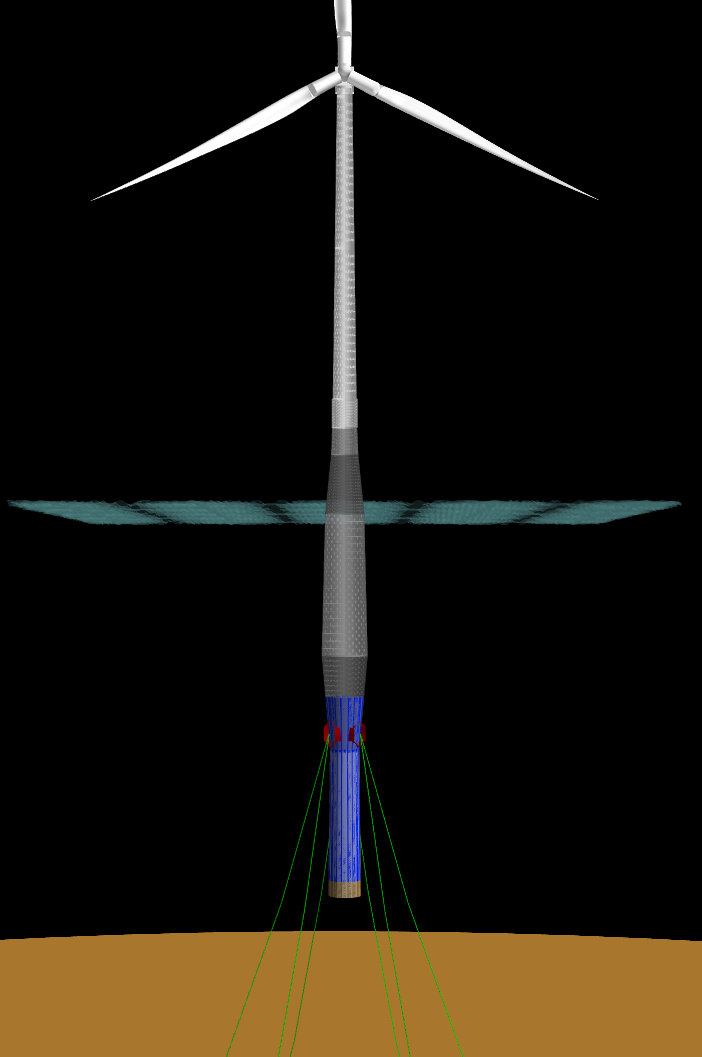
\includegraphics[height=2.25in]{spar-mass1.png}
    \caption{Mass-optimized}
  \end{subfigure}
  \begin{subfigure}[b]{0.24\linewidth}
    \centering 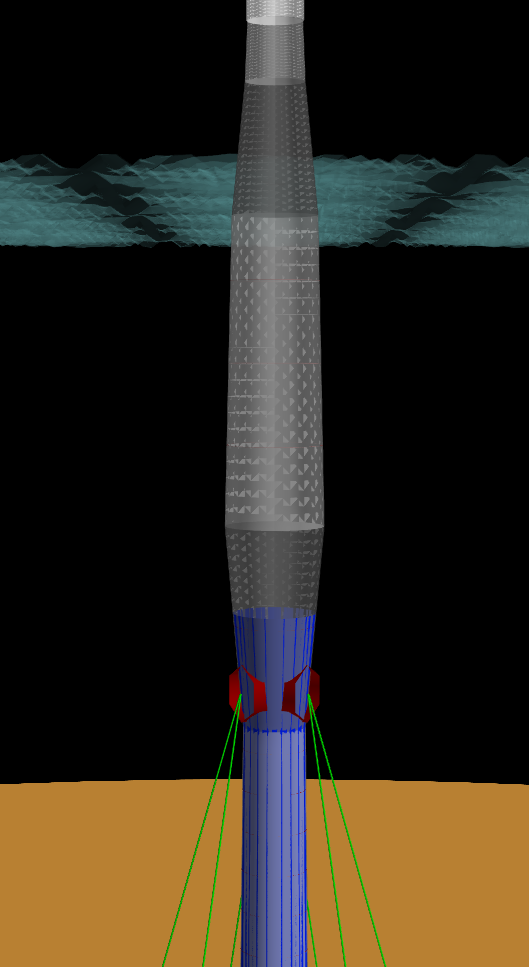
\includegraphics[height=2.25in]{spar-mass2.png}
    \caption{Mass-optimized}
  \end{subfigure}
  \begin{subfigure}[b]{0.24\linewidth}
    \centering 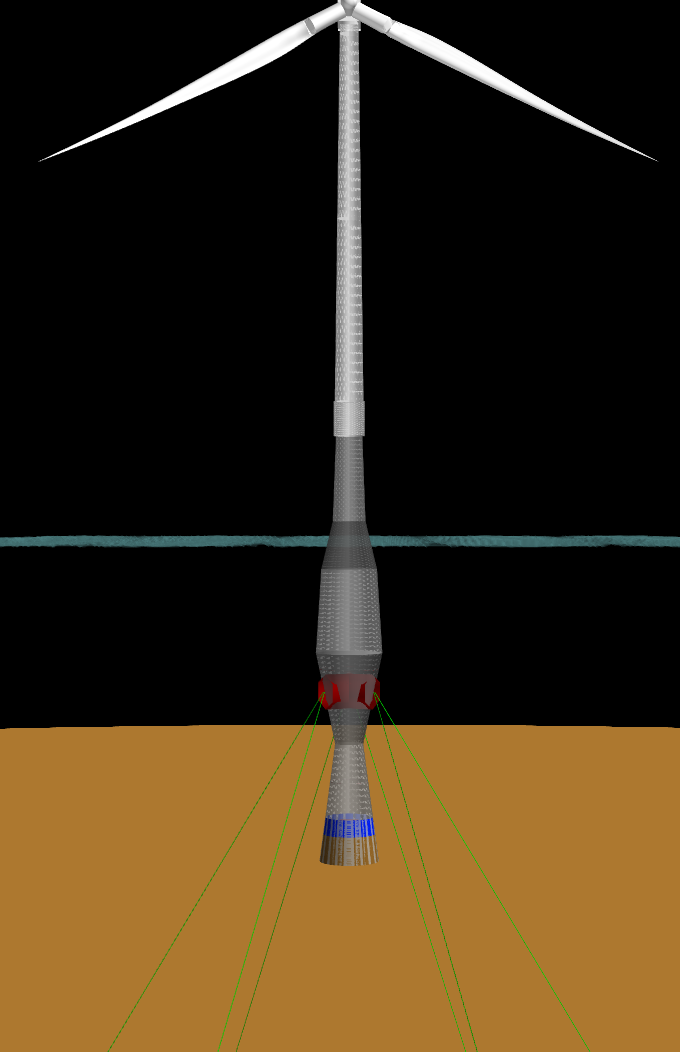
\includegraphics[height=2.25in]{spar-cost1.png}
    \caption{Cost-optimized}
  \end{subfigure}
  \begin{subfigure}[b]{0.24\linewidth}
    \centering 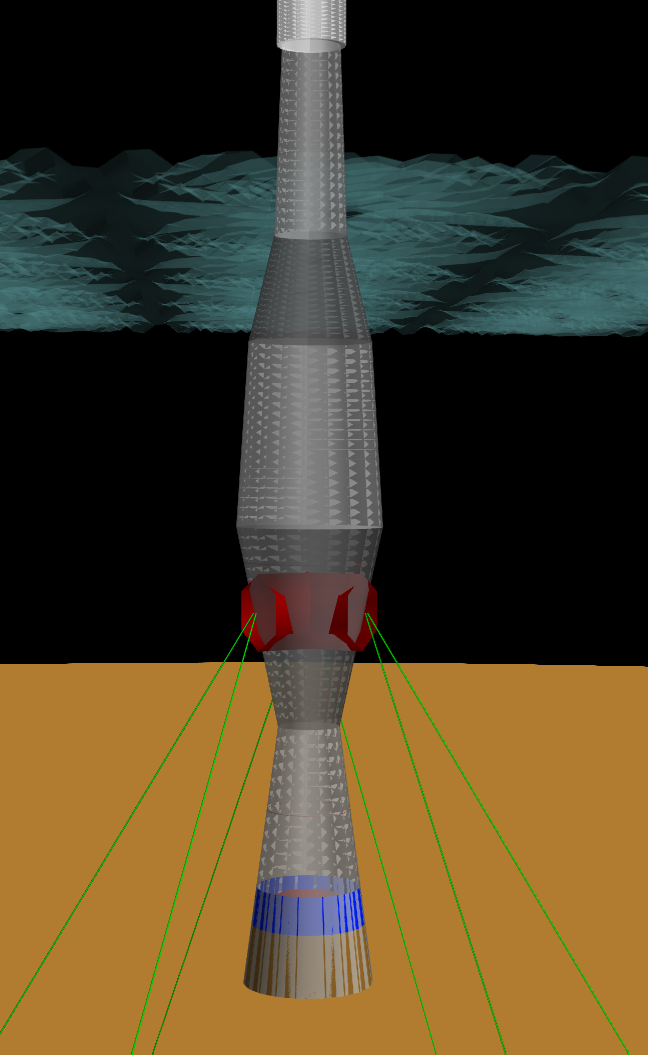
\includegraphics[height=2.25in]{spar-cost2.png}
    \caption{Cost-optimized}
  \end{subfigure}
  \caption{Views of optimized spar substructure designs.}
  \label{fig:spar-design}
\end{figure}

The optimized spar designs are shown in Figure \ref{fig:spar-design},
with obvious differences between the mass-optimized and cost-optimized
designs.  The mass-optimized design has a deeper draft with a narrower
diameter and significantly more water ballast.  The cost-optimized
design has a wider diameter with a shorter draft, more permanent
ballast, and less water ballast.  The differences are driven by the fact
that water ballast is not counted as part of the manufactured mass, so
when minimizing mass, the optimizer has traded permanent for water
ballast.  To ensure stability, since water ballast is less dense than
permanent ballast, a deeper draft was needed.  In contrast, when
optimizing for cost, a shorter draft means less rolled steel
columns, which are expensive, and thus the heavier, permanent ballast is
required for stability.

Both designs have a number of similarities as well.  The column diameter
narrows slightly near the mooring attachment points.  Also, there are
three mooring attachment points, with two catenary lines per connection
for a total of six lines and anchors.

\subsubsection{Optimized Semisubmersible Design}

\begin{figure}[htb]
  \begin{subfigure}[b]{0.29\linewidth}
    \centering 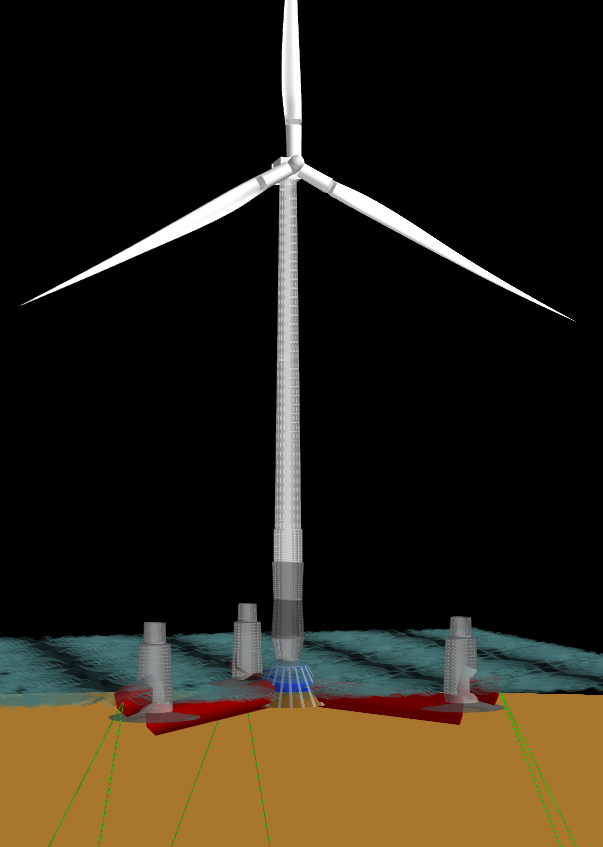
\includegraphics[height=2.25in]{semi-mass1.png}
    \caption{WISDEM semisubmersible}
  \end{subfigure}
  \begin{subfigure}[b]{0.40\linewidth}
    \centering 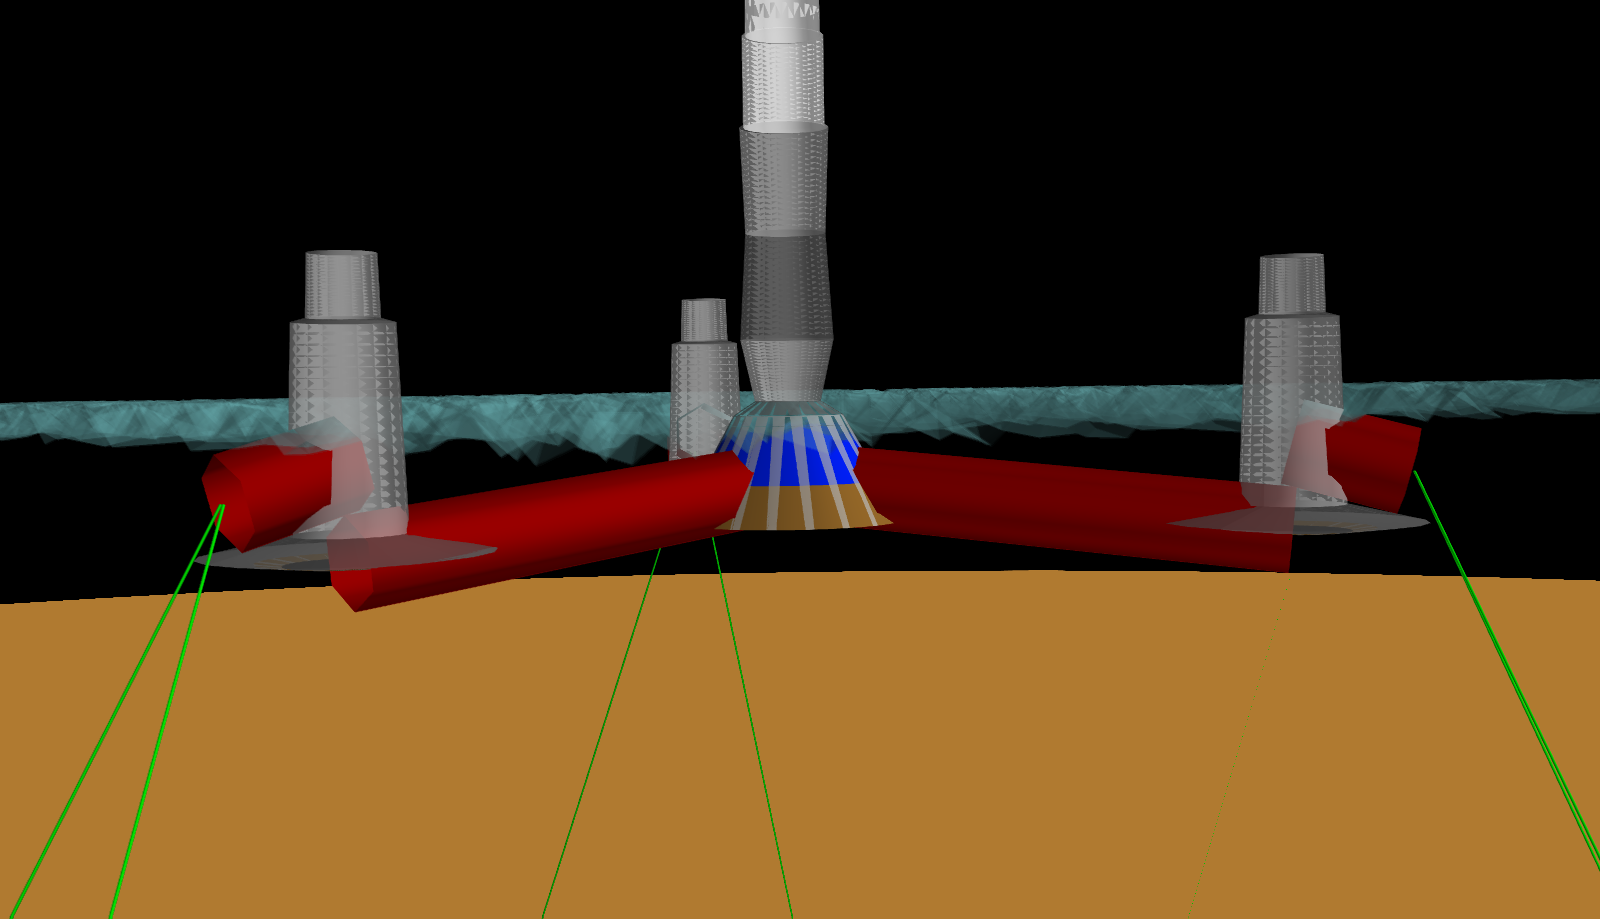
\includegraphics[width=0.95\textwidth]{semi-mass2.png}
    \caption{WISDEM semisubmersible}
  \end{subfigure}
  \begin{subfigure}[b]{0.29\linewidth}
    \centering 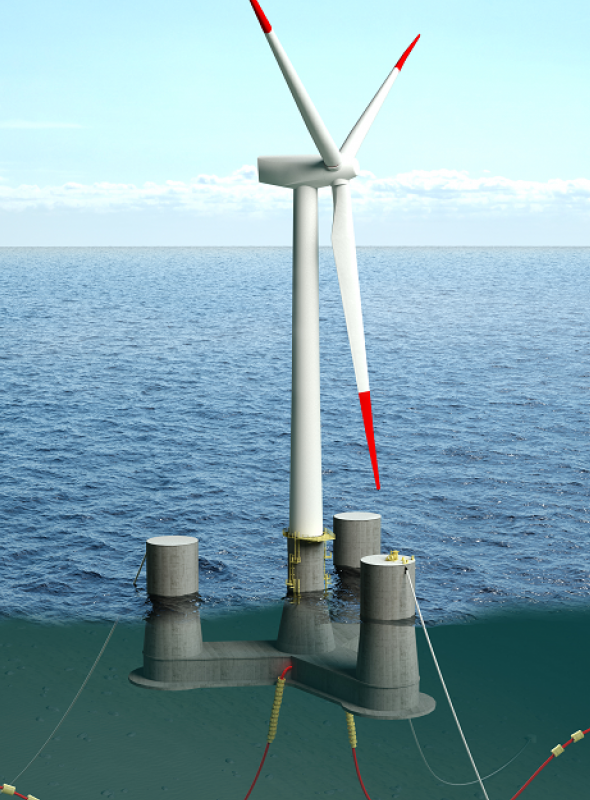
\includegraphics[height=2.25in]{oo-star.png}
    \caption{OO-Star Wind Floater}
  \end{subfigure}
  \caption{Views of semisubmersible substructure optimized for minimal
    substructure mass (not including the mooring system) in (a) and (b).
    OO-Star Wind Floater design by Dr.techn.Olav Olsen for the LIFES50+
    project, a European Horizon 2020 funded program, in (c).}
  \label{fig:semi-mass}
\end{figure}

The optimized semisubmersible design is shown in Figure
\ref{fig:semi-mass}a--b.  In this case, the mass- and cost-optimized
designs look nearly identical, so only one is shown (mass-optimized).
There are three offset columns that sit \unit[53.8]{m} away from the
central column and are connected with a single pontoon.  Near
the bottom, the diameter flares to add some permanent ballast without a
significant increase in column length.  Two catenary mooring lines
attach to each offset column.  The main column has a bell-bottom shape
at the keel with approximately equal volumes of permanent and water
ballast.

It is interesting to compare the semisubmersible design created by
WISDEM to other semisubmersible designs created for the DTU
\unit[10]{MW} reference turbine.  The LIFES50+ project generated a few
candidate substructure designs using the same reference turbine, two of
which were semi-submersibles.  One of those designs, the OO-Star Wind
Floater created by Dr.techn.Olav Olsen, a Norwegian marine consulting
company, has a similar configuration and is shown in Figure
\ref{fig:semi-mass}c. The similarities are especially interesting given the
low-fidelity resolution of the physics and the many simplifying
assumptions used in \textit{FloatingSE}. Unfortunately, despite the
configuration similarities, the OO-Star Wind Floater is made out of
concrete, instead of steel, so direct comparison of dimensions and
weights is not practical.

\subsubsection{Optimized Tension Leg Platform Design}

\begin{figure}[htb]
  \begin{subfigure}[b]{0.24\linewidth}
    \centering 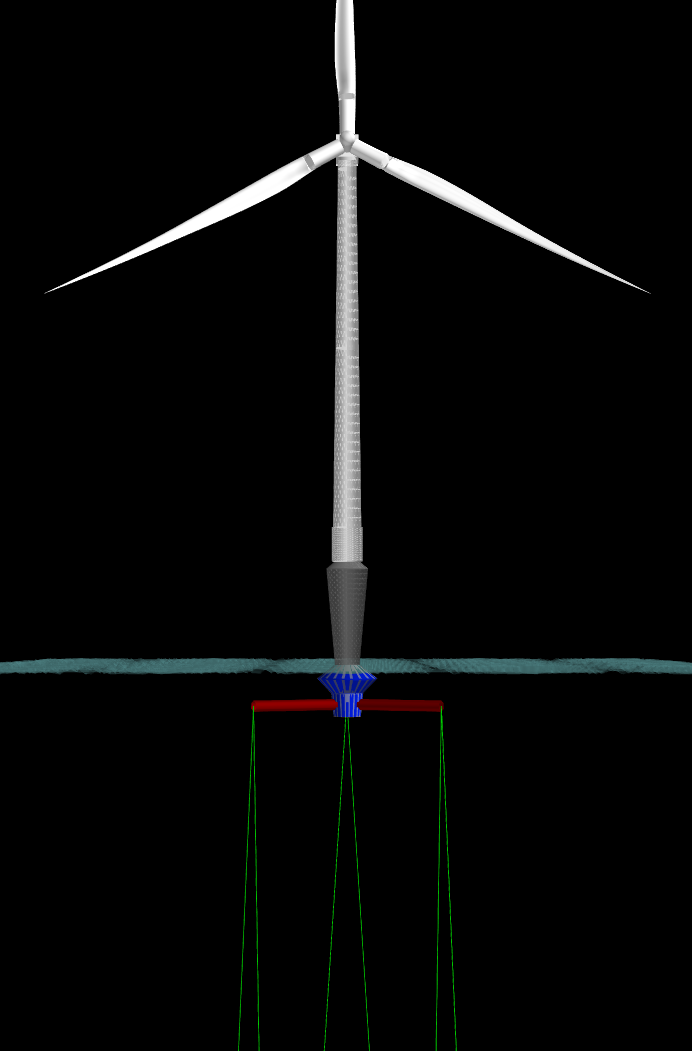
\includegraphics[height=2in]{tlp-mass1.png}
    \caption{Mass-optimized}
  \end{subfigure}
  \begin{subfigure}[b]{0.24\linewidth}
    \centering 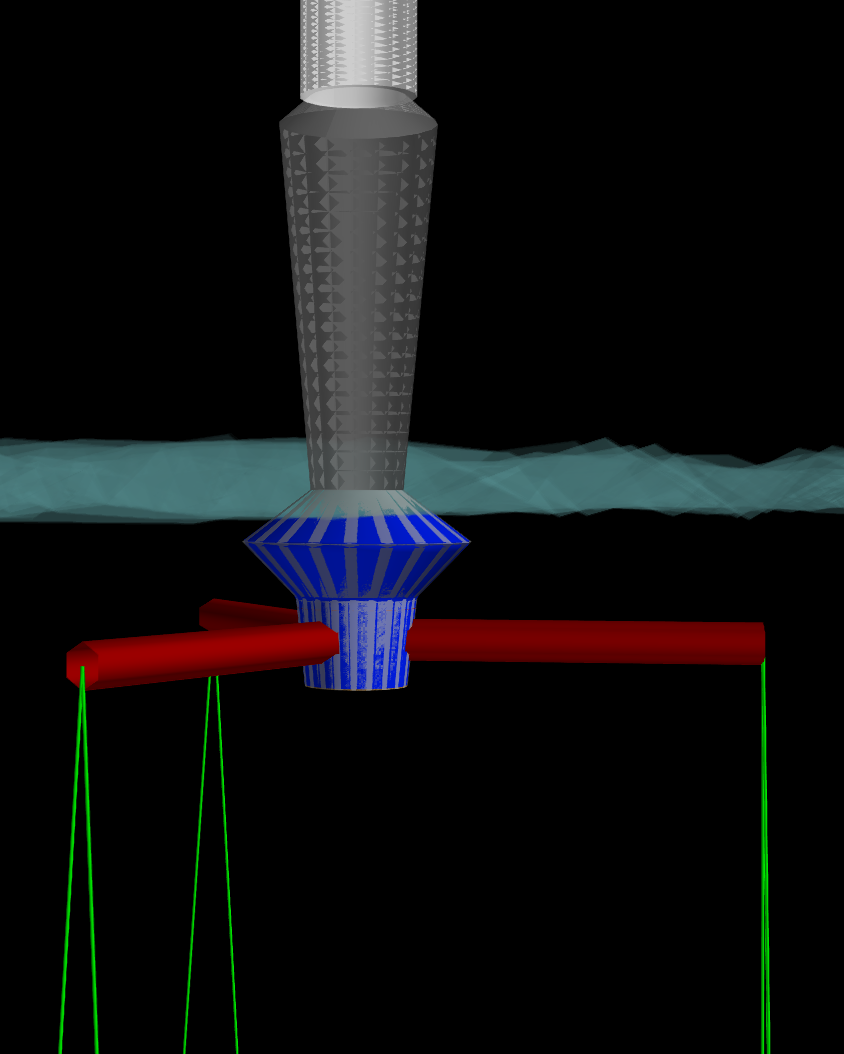
\includegraphics[height=2in]{tlp-mass2.png}
    \caption{Mass-optimized}
  \end{subfigure}
  \begin{subfigure}[b]{0.24\linewidth}
    \centering 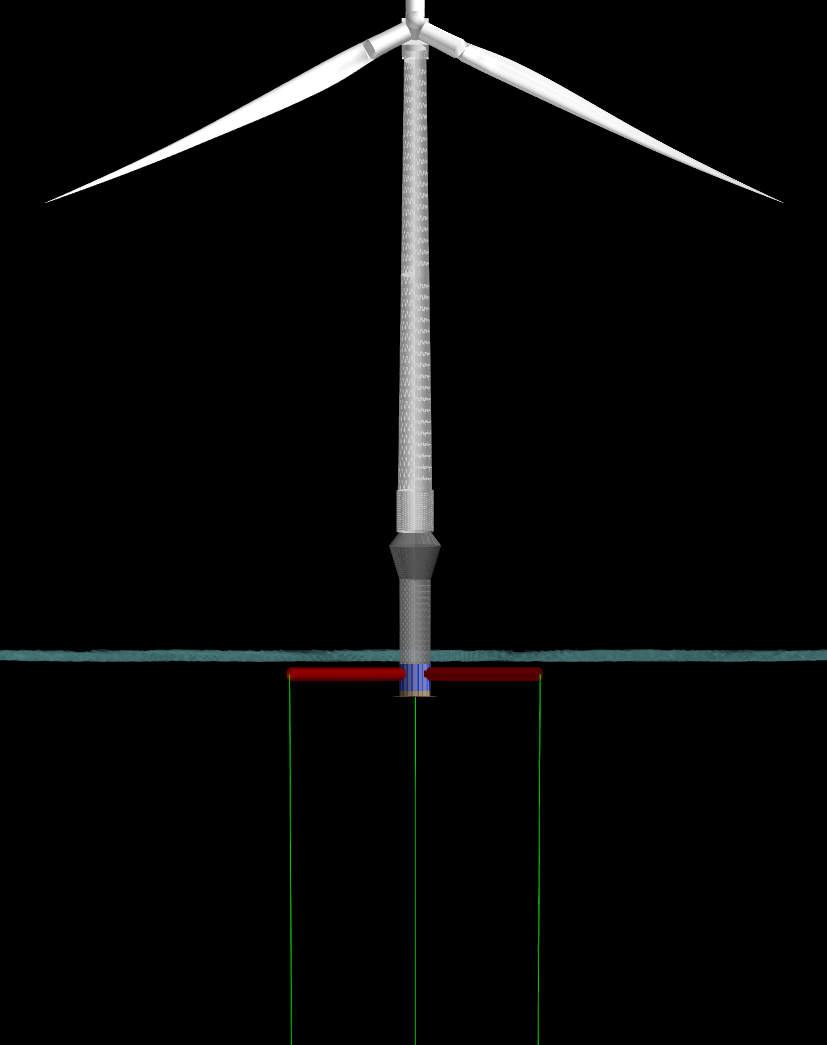
\includegraphics[height=2in]{tlp-cost1.png}
    \caption{Cost-optimized}
  \end{subfigure}
  \begin{subfigure}[b]{0.24\linewidth}
    \centering 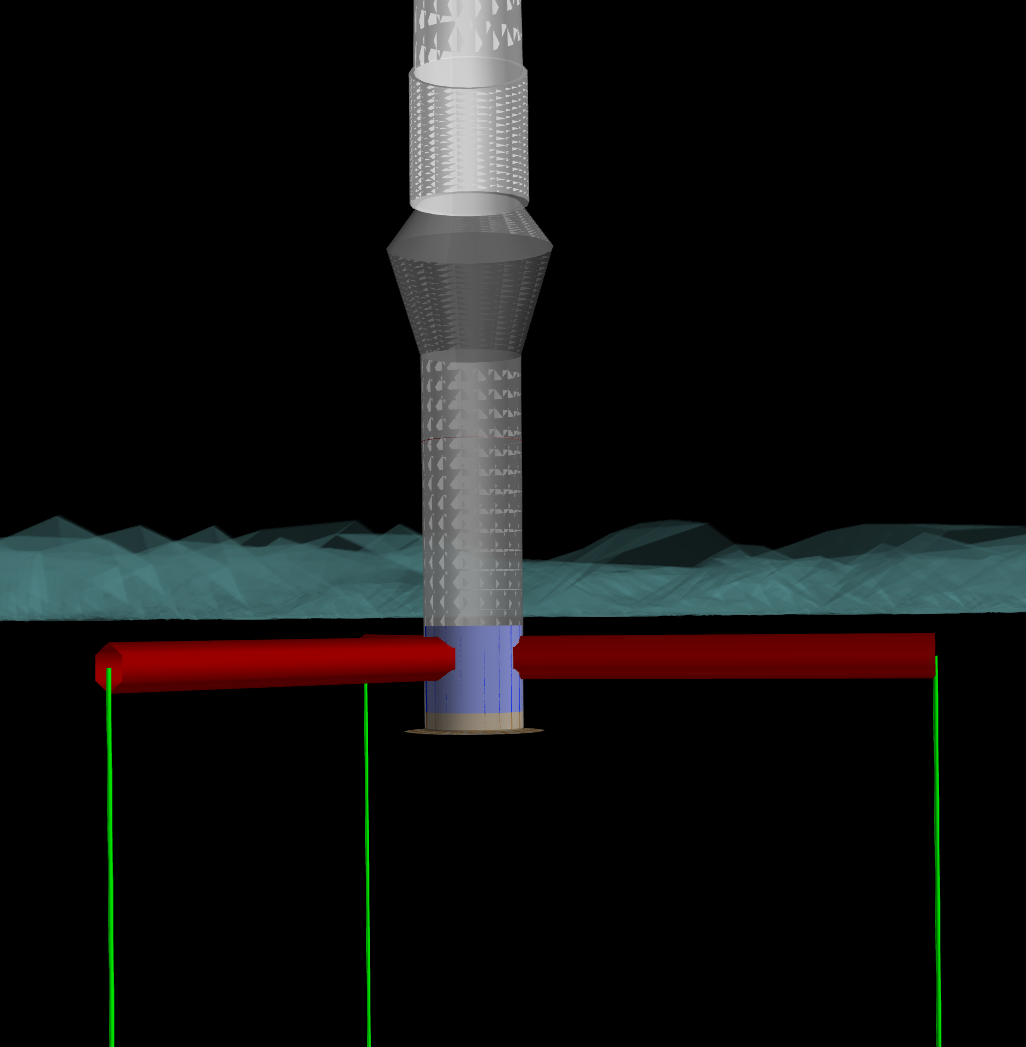
\includegraphics[height=2in]{tlp-cost2.png}
    \caption{Cost-optimized}
  \end{subfigure}
  \caption{Views of optimized TLP substructure designs.}
  \label{fig:tlp-design}
\end{figure}

The TLP designs are shown in Figure \ref{fig:tlp-design}, and
differences between the mass- and cost-optimized geometries are once
again obvious.  The mass-optimized design has three legs with two taut
mooring lines per attachment and, as with the spar design, extensive use
of water ballast.  The legs extend \unit[30.5]{m} from the centerline to
the mooring attachment points.  In contrast, the cost-optimized design
has a single taut mooring line per attachment and requires very little
ballast.  This difference is driven primarily by the decision to not
include the mooring system into the substructure mass budget.  Table
\ref{tbl:optdesign} shows that the total mooring downward force on the
structures.  Despite needing sturdier legs to support those mooring
loads, shifting additional stability burden to the mooring system allows
for a lighter structure.

\subsection{Sensitivity Studies}

\begin{table}[htbp]
  \begin{center}
    {\small
    \caption{Nacelle and RNA mass perturbations for design sensitivity studies.}
    \label{tbl:delta_rna}
    \begin{tabular}{cccc}
      \hline
      \textbf{Nacelle Perturbation} & \textbf{Nacelle Mass [\unit{kg}]} & \textbf{RNA Mass [\unit{kg}]} &
      \textbf{RNA Perturbation}\\ \hline \hline
      Nominal & 446,036 & 672,301 & -\\
      +10\% & 490,640 & 716,904 & +6.6\%\\
      -10\% & 401,433 & 627,697 & -6.6\%\\
      -25\% & 334,527 & 560,791 & -16.6\%\\
      -33\% & 297,506 & 523,770 & -22\%\\
      -50\% & 223,018 & 449,282 & -33\%\\ \hline
    \end{tabular}
    }
  \end{center}
\end{table}

For the sensitivity studies, the optimized designs shown above were
taken as baseline starting points.  Then, the DTU 10MW reference turbine
nacelle mass was perturbed away from its nominal value by the
parameterization shown in Table \ref{tbl:delta_rna}.  Next, each design
was re-optimized at the new nacelle mass value using the Nelder-Mead
Simplex algorithm.  All continuous design variables, constraints, and
their bounds were kept consistent from the baseline optimization.  The
integer design variables were dropped to focus on a neighborhood search.
As above, two sets of sensitivity optimizations were performed with
different objective functions: one for substructure mass (not including
the mooring system), and one for total substructure mass (including the
mooring system).

\subsubsection{Caveats}
All of the caveats regarding substructure design mentioned above still
apply to the design sensitivity analysis as well.  In addition to those,
there are a couple of other points to keep in mind when considering the
results shown here,
\begin{itemize}
\item Design variables did not include the tower, a key structural
  component that would change with nacelle mass.  Had tower design
  variables been included, the total mass reductions would likely have
  been higher;
\item Cost sensitivity is for substructure capital cost only.  Other
  costs such as those captured in a balance of station or operational
  model would likely demonstrate different sensitivities;
\item The cost rates listed in Table \ref{tbl:factors} are notional,
  but still determine the priorities of the cost-optimized solutions and
  break-even cost points.  Thus, the final break-even costs should also
  be considered notional;
\item Just as the optimized designs reflect the assumptions and
  fidelity of \textit{FloatingSE}, so too do the sensitivity study
  results.  So, if the underlying assumptions or fidelity improve in
  the future, the key points determined here may shift.
\end{itemize}


\subsubsection{Mass-Optimized Design Sensitivity}
The sensitivity of substructure mass (not including the mooring system),
for all three substructure types, with respect to changes in nacelle
mass is shown in Figure \ref{fig:mass-mass}.  Absolute values of mass
changes are shown in Figure \ref{fig:mass-mass}a and percentage changes
are in Figure \ref{fig:mass-mass}b.  Reading from right to left, between
the three substructure types, the slopes are all initially similar, but
not exactly the same.  The slope of the spar curve appears the most
linear and the steepest, with approximately \unit[1.5--2]{kg} of
substructure mass removed for each \unit[1]{kg} of mass removed from the
nacelle.  The slope for the TLP is shallower, approximately
\unit[1]{kg} of substructure mass removed for each \unit[1]{kg} of
mass removed from the nacelle.  The slope of the semisubmersible curve is
the most interesting.  For small deviations around the nominal point,
the slope of the semisubmersible curve nearly matches that of the spar,
but at more significant mass decreases, the slope flattens out and the
substructure mass is relatively constant.  This implies that the
substructure design is more heavily bracketed by constraints and design
variable bounds.

\begin{figure}[htb]
  \begin{subfigure}[b]{0.49\linewidth}
    \centering 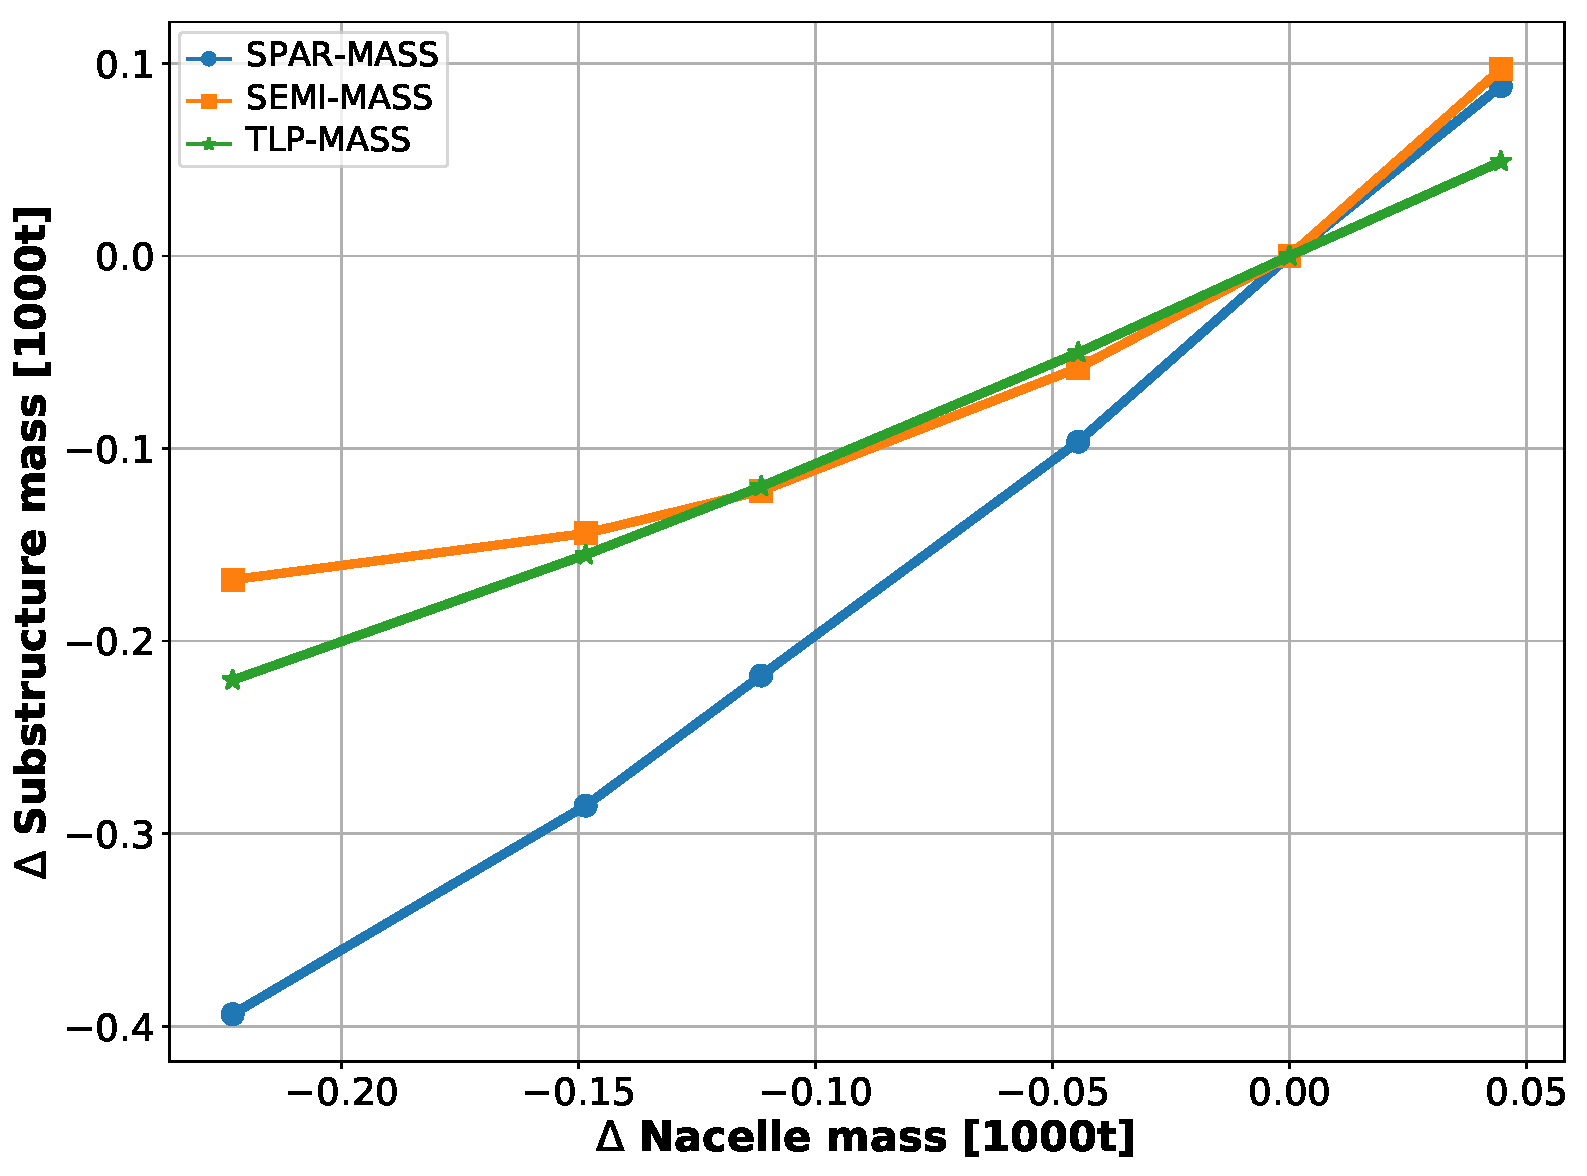
\includegraphics[width=0.9\textwidth]{mass-mass}
    \caption{Absolute mass changes, mass-optimized}
  \end{subfigure}
  \begin{subfigure}[b]{0.49\linewidth}
    \centering 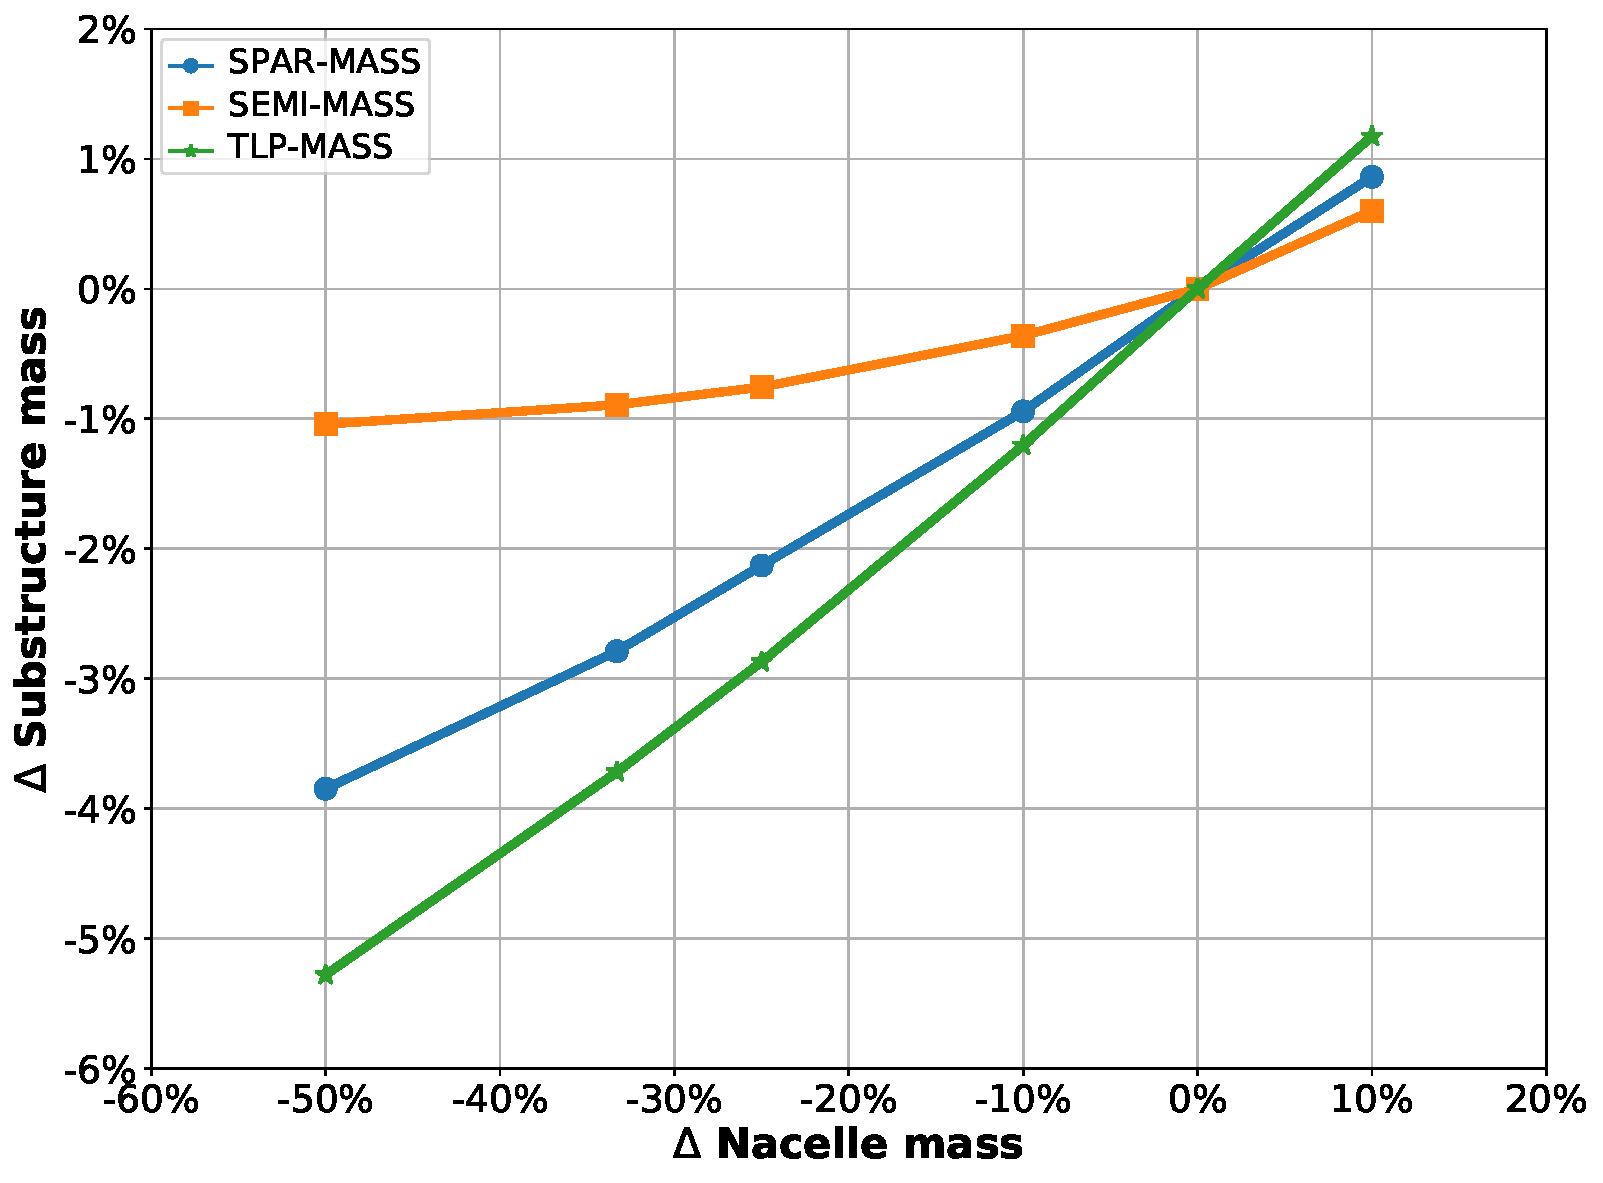
\includegraphics[width=0.9\textwidth]{mass-mass_perc}
    \caption{Percent mass changes, mass-optimized}
  \end{subfigure}
  \caption{Sensitivity of substructure mass (without mooring system)
    relative to mass changes in nacelle for mass-optimized baseline designs.}
  \label{fig:mass-mass}
\end{figure}

The mass sensitivities, shown in
Figure \ref{fig:mass-mass}, are really summary statistics as the
substructure is comprised of multiple components.  The percentage change
of some other metrics are shown in Figure \ref{fig:mass-other}.  Note
that the curves for these other metrics are not smooth because they were
not the objective function, so they were not monitored or controlled by the
algorithm.  For instance, the total displacement (Figure
\ref{fig:mass-other}a), the submerged volume of the substructure, does
not follow the same trend lines as the mass reductions in Figure
\ref{fig:mass-mass}b.  The total displacement of the spar does decrease
as the mass of the nacelle decreases, meaning the tapered column becomes
narrower, but the trend is not nearly as linear as the mass sensitivity.
This is likely due to the fact that the total displacement is closely
tied to some of the stability constraints, such as metacentric height,
and so cannot vary in the same regard.

\begin{figure}[htb]
  \begin{subfigure}[b]{0.49\linewidth}
    \centering 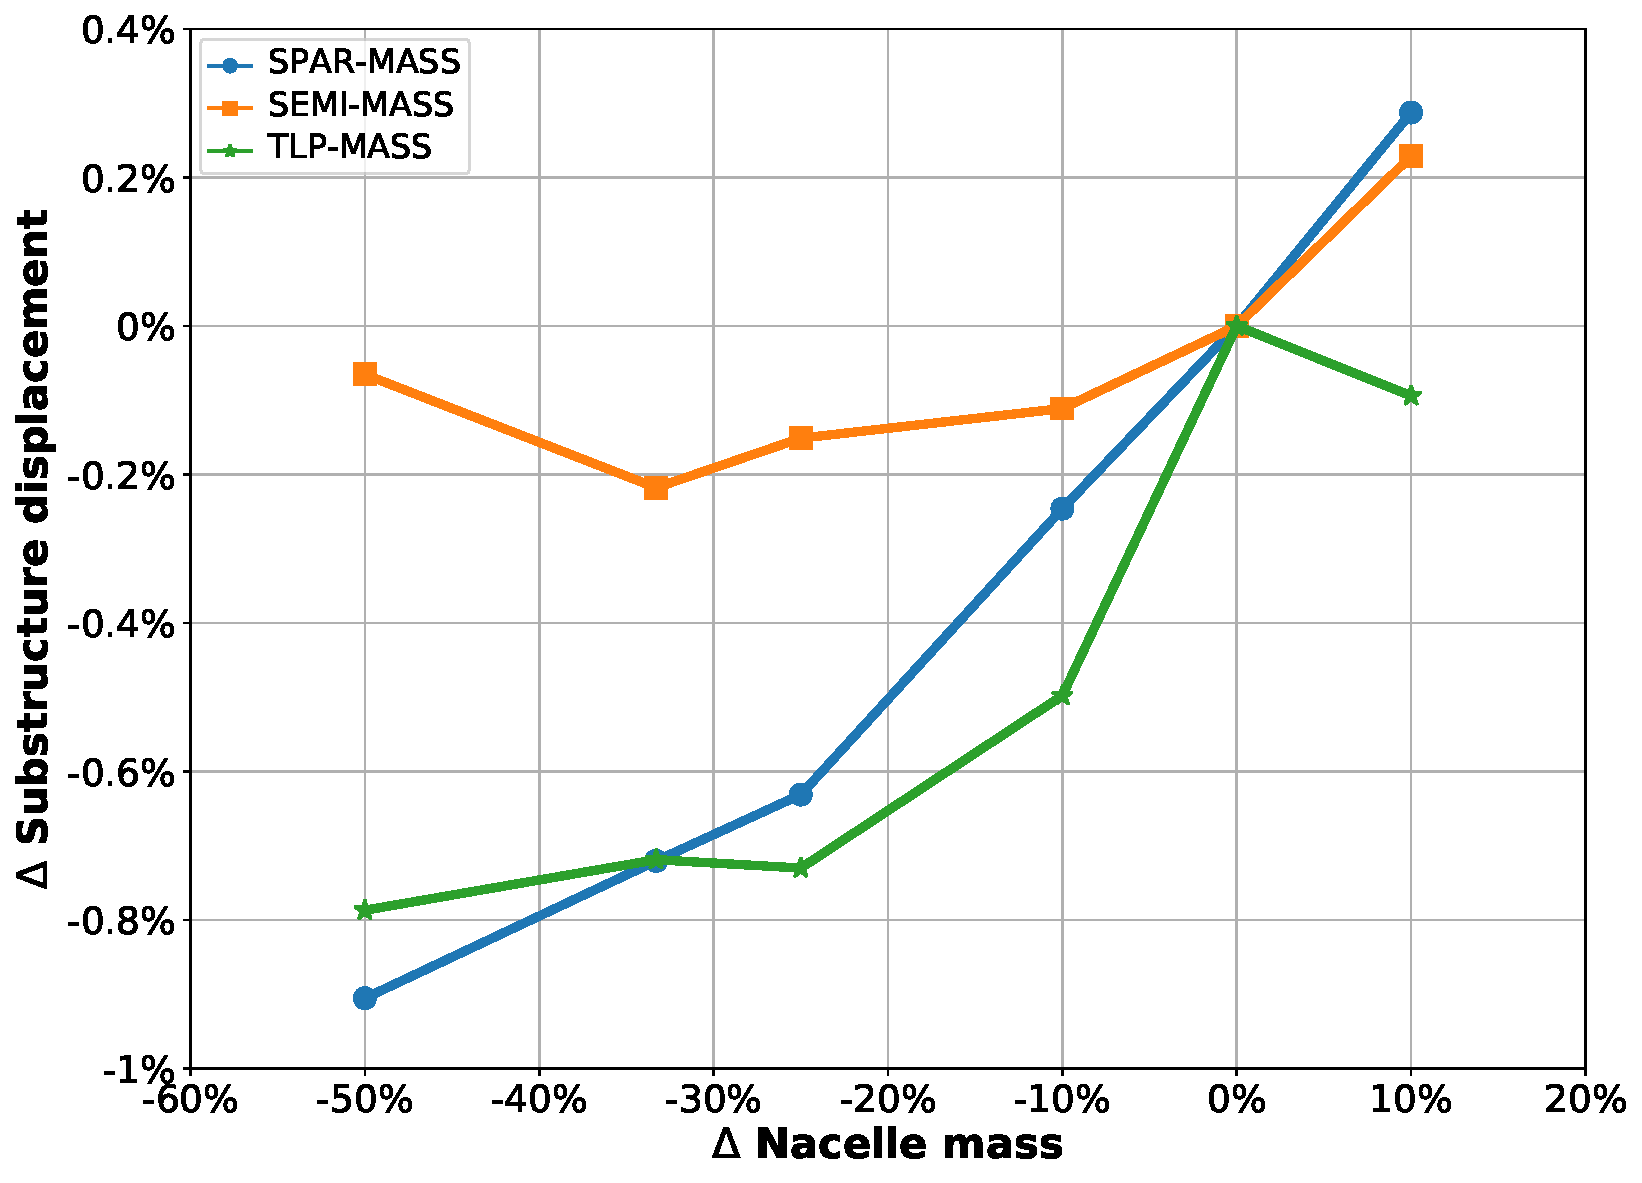
\includegraphics[width=0.9\textwidth]{mass-volume_perc}
    \caption{Displaced volume}
  \end{subfigure}
  \begin{subfigure}[b]{0.49\linewidth}
    \centering 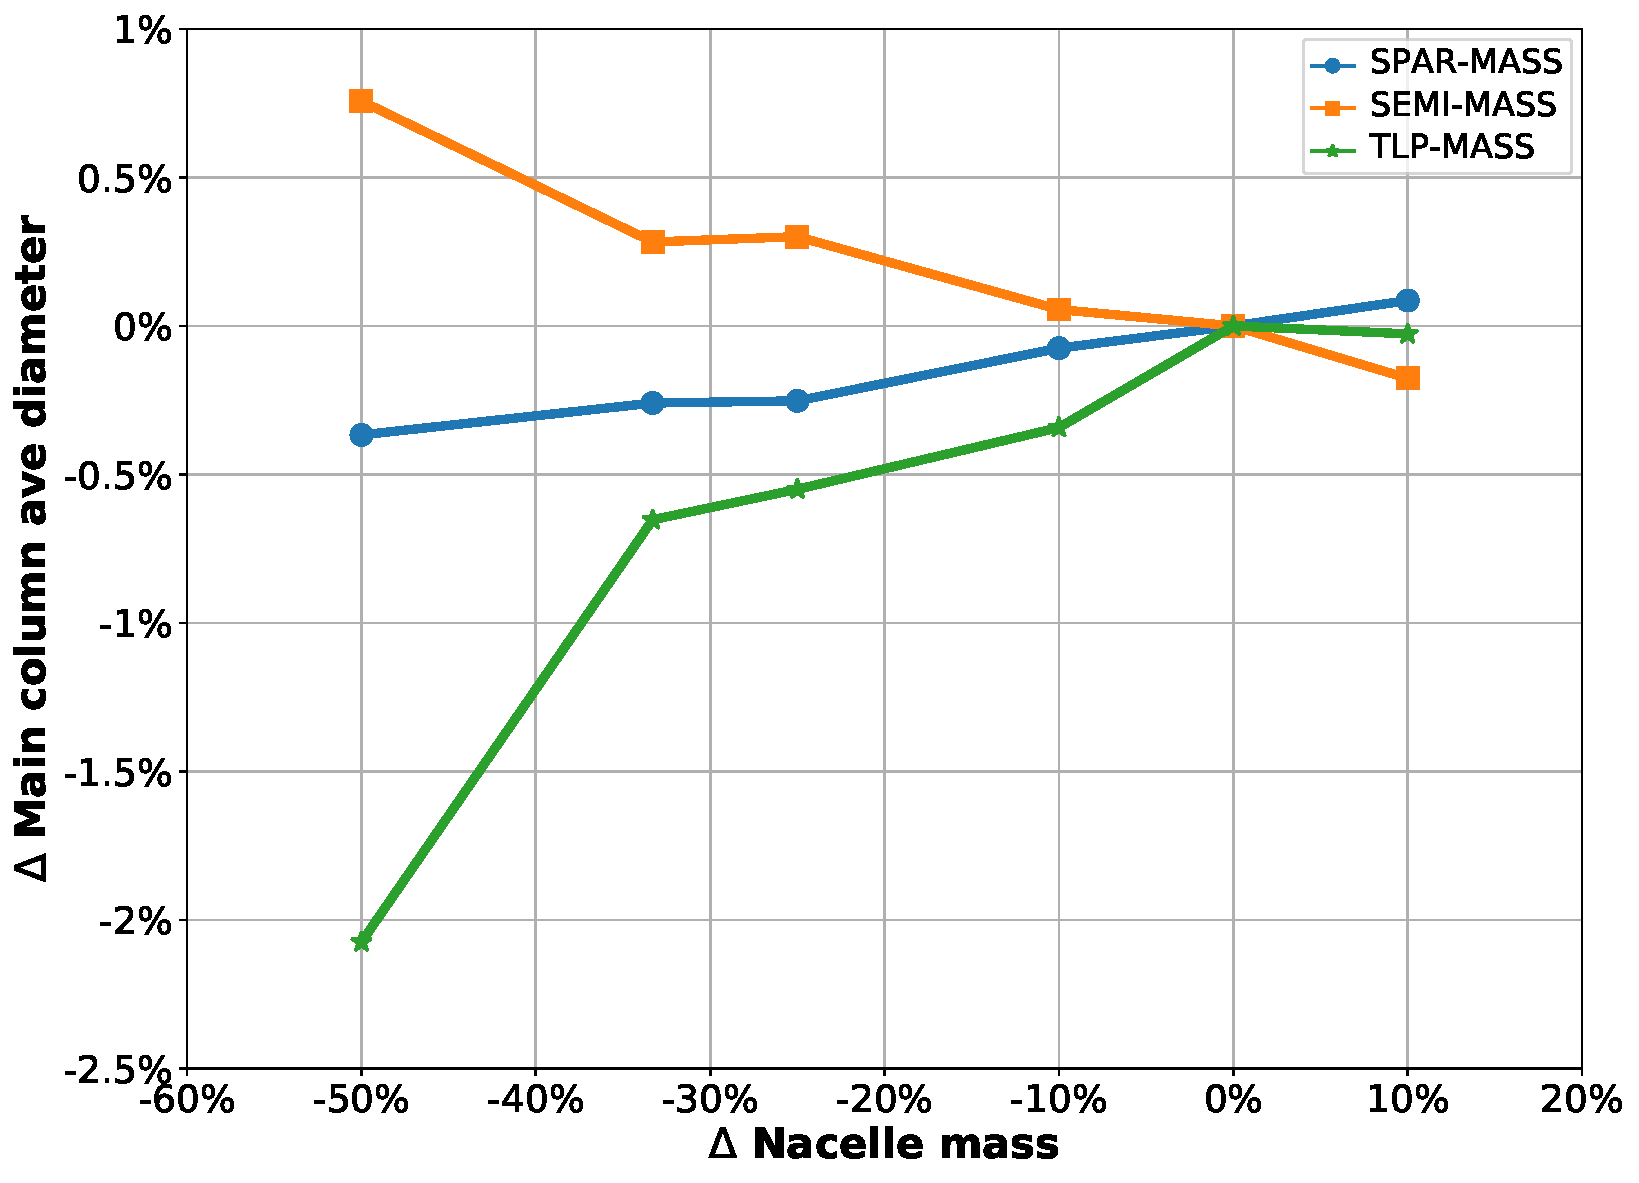
\includegraphics[width=0.9\textwidth]{mass-baseaved_perc}
    \caption{Main column average diameter}
  \end{subfigure}\\
  \begin{subfigure}[b]{0.49\linewidth}
    \centering 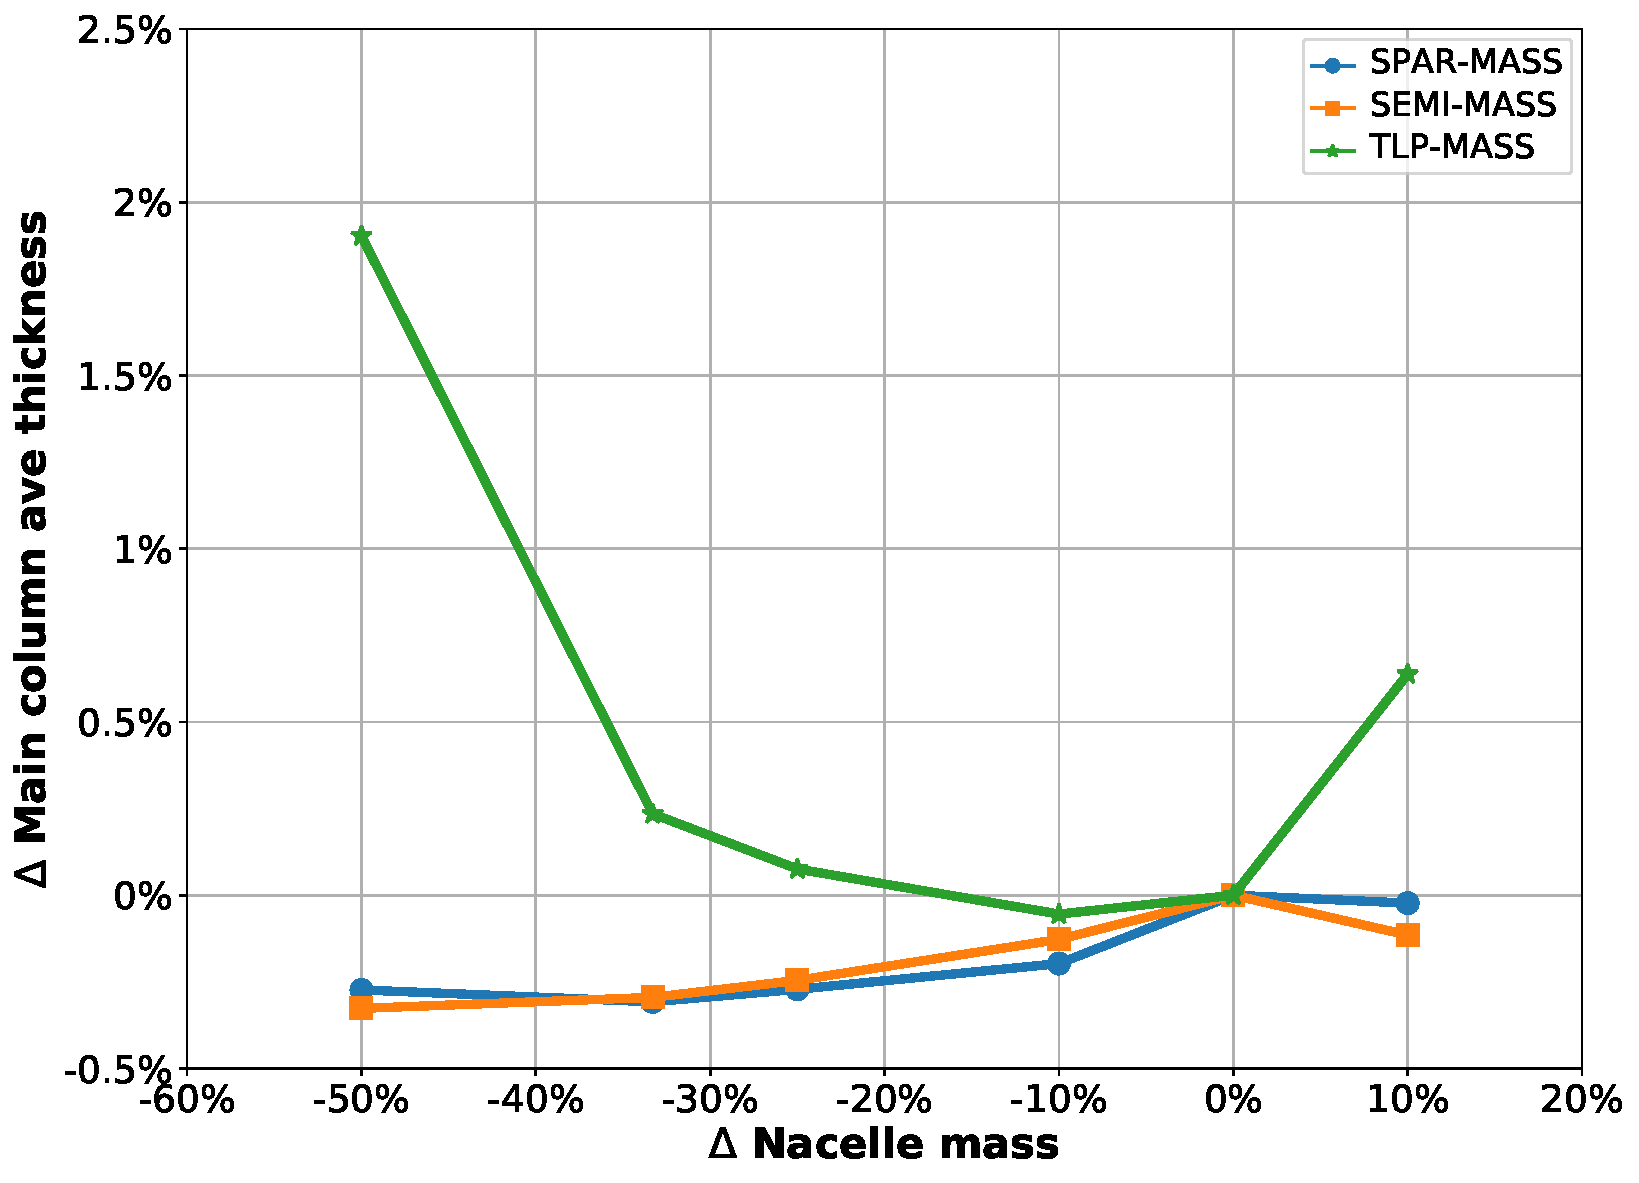
\includegraphics[width=0.9\textwidth]{mass-baseavet_perc}
    \caption{Main column average thickness}
  \end{subfigure}
  \begin{subfigure}[b]{0.49\linewidth}
    \centering 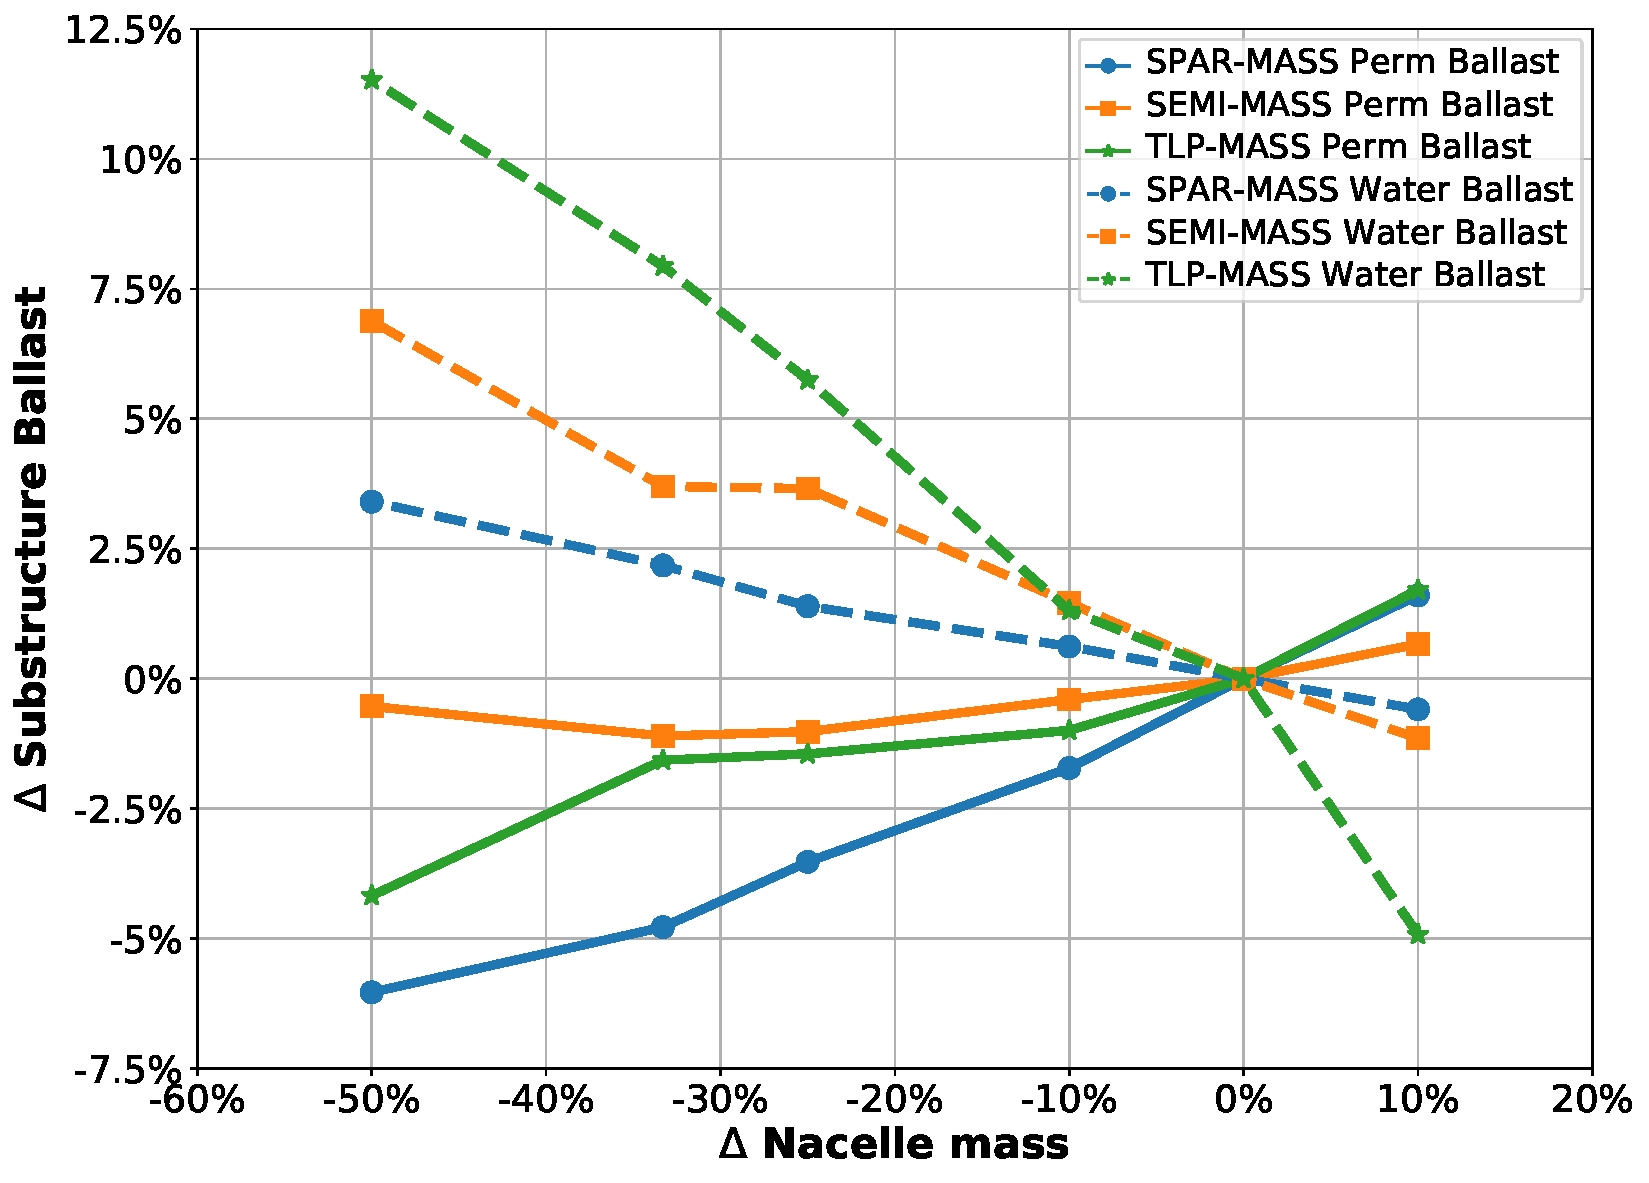
\includegraphics[width=0.9\textwidth]{mass-allball_perc}
    \caption{Permanent (solid) and water (dashed) ballast}
  \end{subfigure}
  \caption{Sensitivity of other substructure metrics (volume, water
    ballast, mooring tension, total cost) relative to mass changes in
    nacelle for mass-optimized baseline designs.}
  \label{fig:mass-other}
\end{figure}

Figures \ref{fig:mass-other}b--c show the change in the average diameter
and thickness of the main column to illustrate how the geometry changes
during the parameterized.  For the spar, as the mass of the nacelle
becomes less, the column becomes both slightly narrower and with
slightly thinner walls.  For the semisubmersible, the diameter stays
roughly constant (or even increases slightly), but the thickness
decreases.  For the TLP, the diameter decreases sharply, but the
thickness increases.

Figure \ref{fig:mass-other}d shows the change in permanent (solid lines)
and water (dashed lines) ballast as the mass in the nacelle decreases.
The percentage changes here are the most pronounced and the shape of the
curves most closely resemble that of the overall mass change in Figure
\ref{fig:mass-mass}b.  This suggests that further converting permanent
ballast into water ballast (which is not counted in the mass budget) is
the dominant trend driving the results of the mass-optimized sensitivity
study.  This is an important trend to keep in mind when interpreting the
change in substructure costs presented below.


\subsubsection{Mass vs.~Cost Scaling}

\begin{figure}[htbp]
  \begin{subfigure}[b]{0.49\linewidth}
    \centering 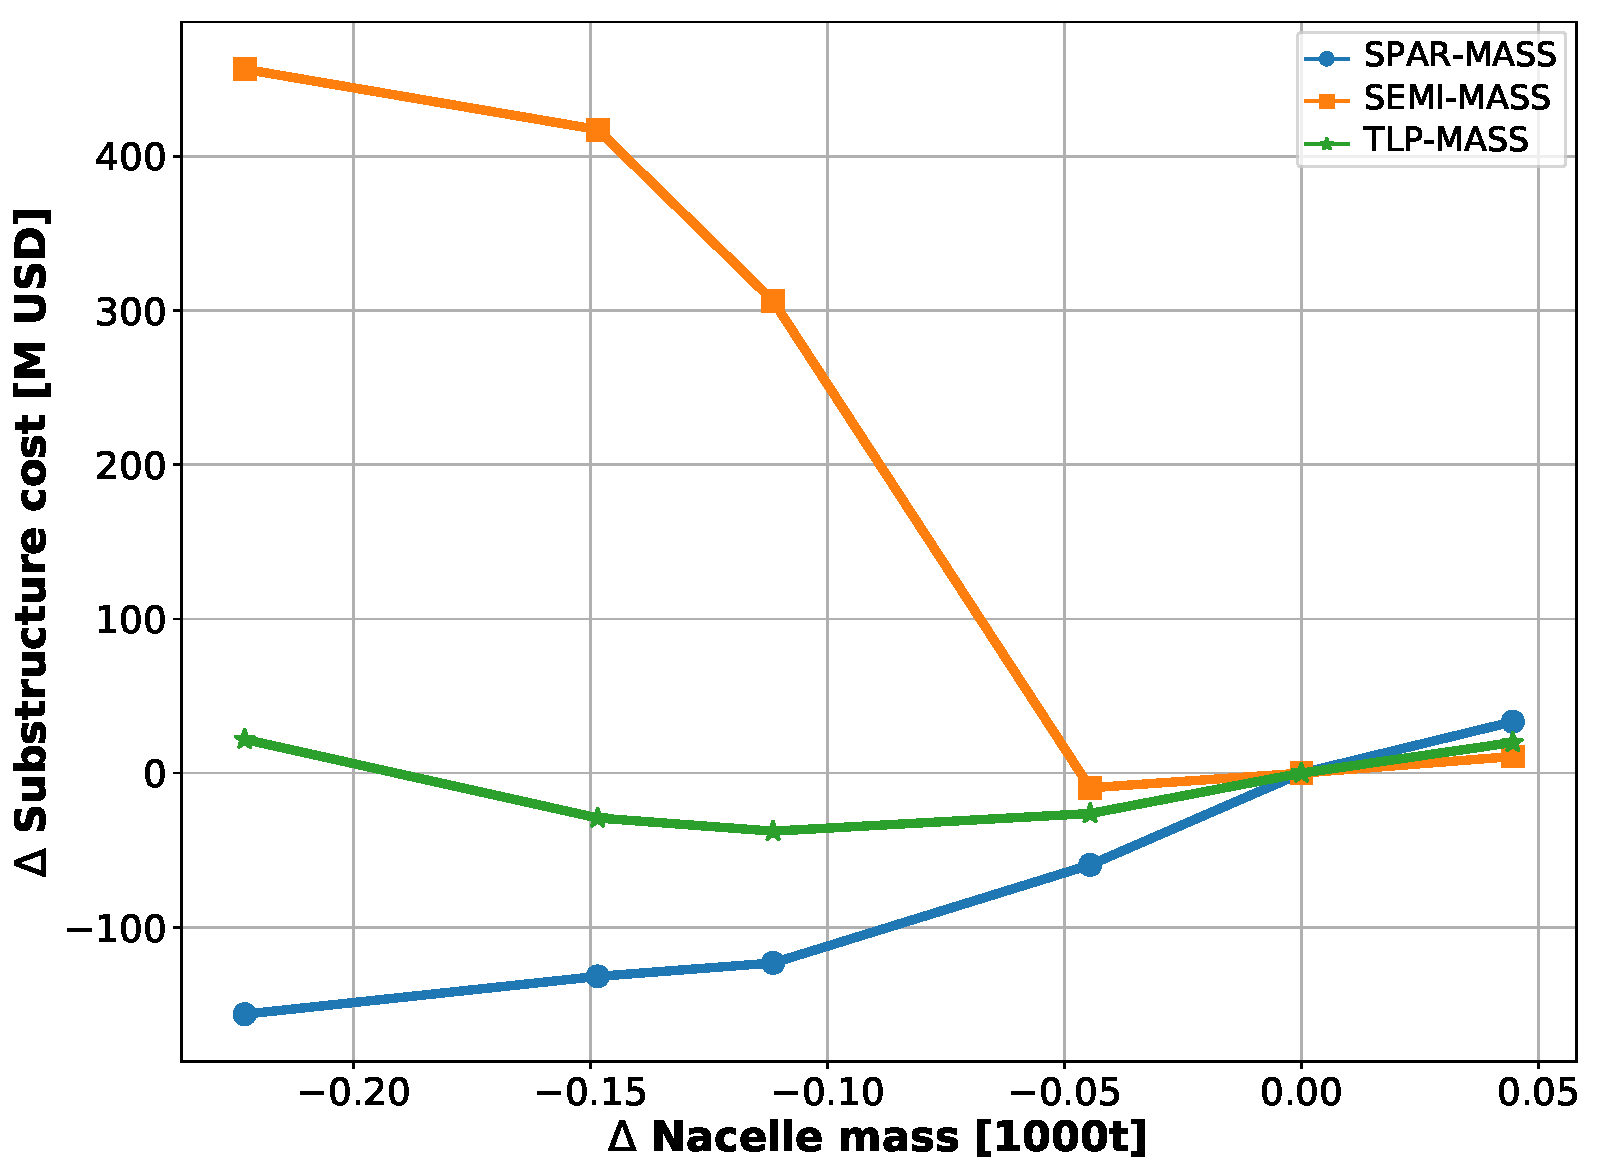
\includegraphics[width=0.9\textwidth]{mass-cost}
    \caption{Absolute cost changes, mass-optimized}
  \end{subfigure}
  \begin{subfigure}[b]{0.49\linewidth}
    \centering 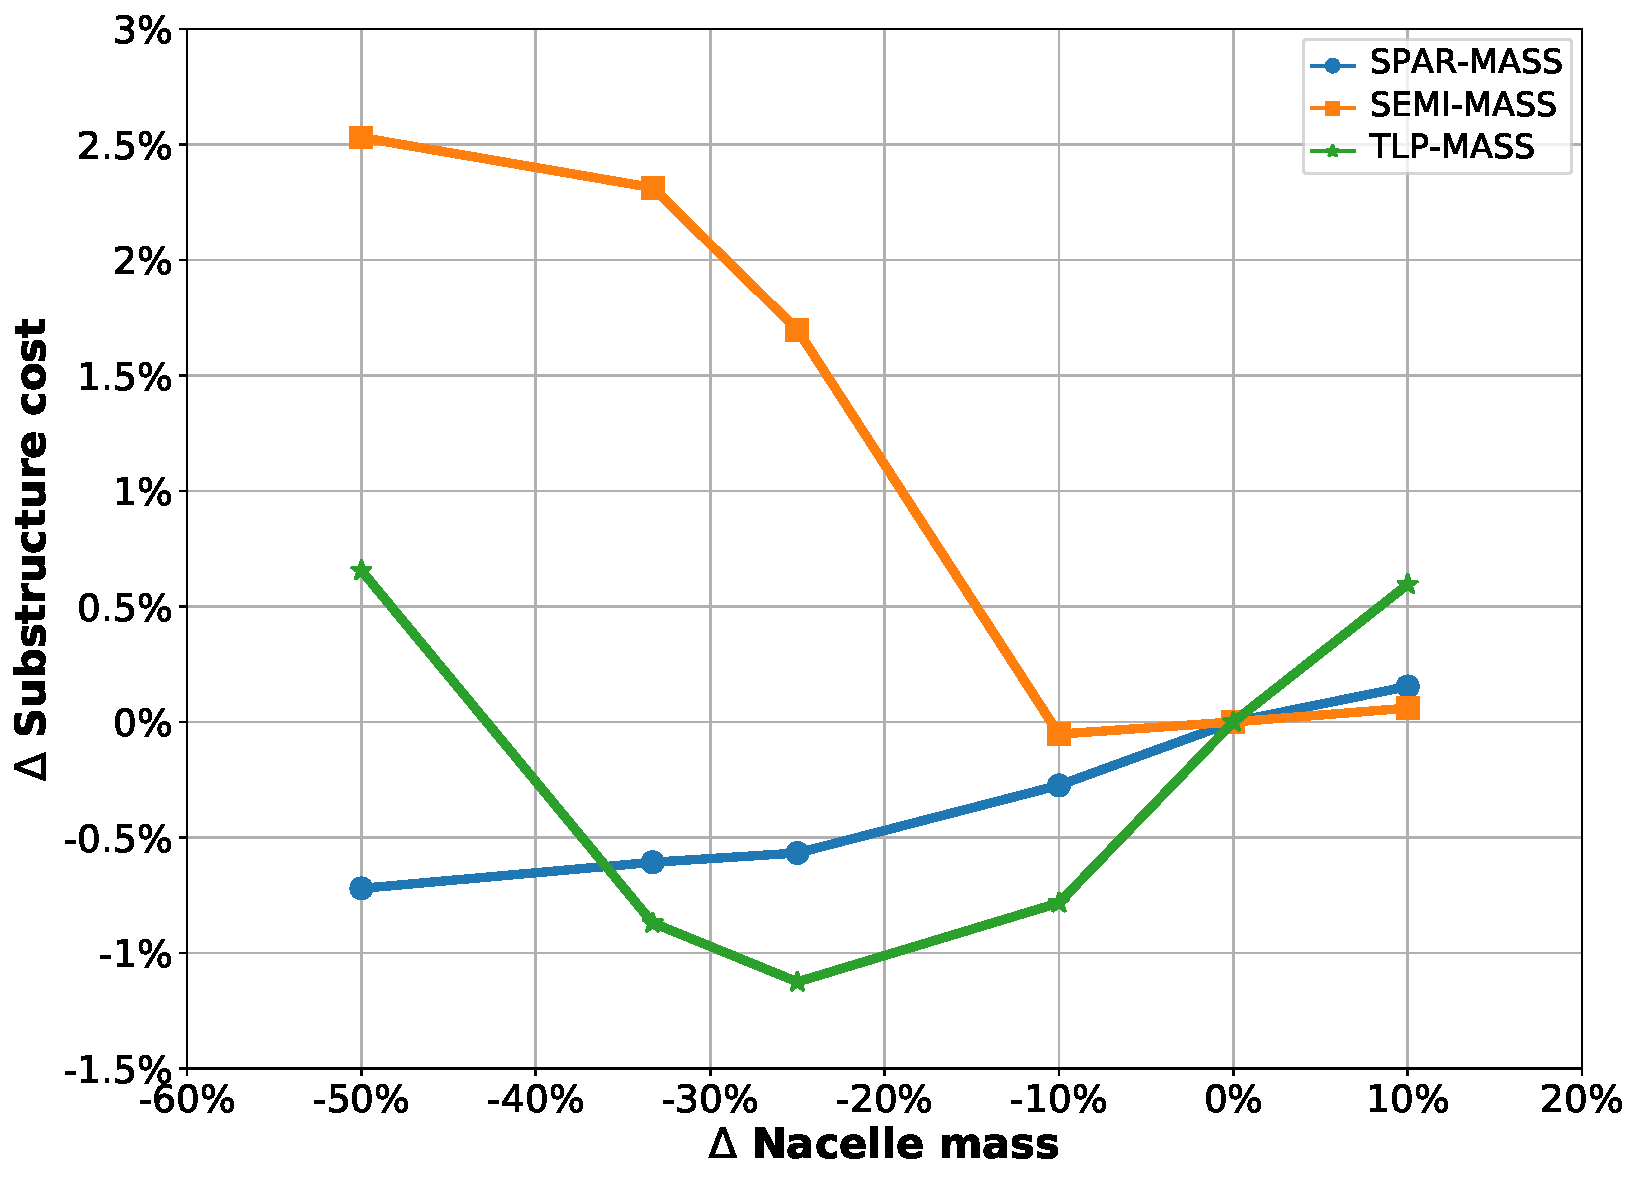
\includegraphics[width=0.9\textwidth]{mass-cost_perc}
    \caption{Percent cost changes, mass-optimized}
  \end{subfigure}\\
  \caption{Sensitivity of substructure cost (with mooring system)
    relative to mass changes in nacelle for mass-optimized baseline designs.}
  \label{fig:mass-cost}
\end{figure}

The change in substructure cost, including the mooring system, for the
mass-optimized designs in the sensitivity study is shown in Figure
\ref{fig:mass-cost} in both absolute and percentage terms.  The results
are, at first, quite surprising, but are consistent with the other
results shown above.  The mass-optimized spar design demonstrates a
mass reduction slope of $1.5--2$ relative to nacelle mass reduction,
which is a reflection of decreases in the spar diameter, thickness, and
permanent ballast.  This leads to a net cost savings of approximately
\$150M for a 50\% reduction in nacelle mass, which is less than 1\% of
the total cost and far from the 4\% reduction in substructure mass.  The
mass-optimized TLP design shows negligible cost savings for all nacelle
mass perturbations, despite a consistent mass reduction slope of $1$.
The mass-optimized semisubmersible design has a small margin for overall
mass reduction since it is tightly constrained, but nevertheless does
achieve measurable reductions over the course of the parameterization.
However, Figure \ref{fig:mass-cost} shows that this mass reduction
actually incurs a cost increase.  This is inconsistent with
expectations, but can be understood through the results in Figure
\ref{fig:mass-other}d and Table \ref{tbl:factors}.  To reduce the mass,
the optimizer has aggressively reduced the amount of permanent ballast
in favor of water ballast.  To maintain stability despite this change,
the column diameter and draft (which was not shown) actually increased
slightly.  While permanent ballast is heavy, it is also inexpensive per
unit mass, whereas rolled steel columns are an order-of-magnitude more
expensive.  Since the mass-optimized design is blind to cost, the
algorithm traded a heavy but cheap ingredient for a lighter but more
expensive ingredient.  This explains the ostensibly counter-intuitive
trends seen in Figure \ref{fig:mass-cost}.

\subsubsection{Cost-Optimized Design Sensitivity}
For a consistent reduction in both substructure mass and cost with
respect to mass reductions in the nacelle, we must look to the
cost-optimized design sensitivity results.  These results are shown in
Figure \ref{fig:cost-cost}.  The reductions of platform mass, shown in
Figures \ref{fig:cost-cost}a--b, are quite linear despite the fact that
the designs are cost-optimized.  The slopes of the lines are actually
about equal to those in Figure \ref{fig:mass-mass}.  The spar has a
slope of approximately $2$, and the TLP still has a slope of about $1$.
The semisubmersible line, however, has a much steeper slope, $1.5$, than
in the mass-optimized case.  It is important to note that these
cost-optimized designs have a different baseline starting point than the
mass-optimized designs and all changes shown are relative.  Thus, while
the mass reduction slope for the semisubmersible design is steeper in
Figure \ref{fig:cost-cost} than Figure \ref{fig:mass-mass}, the
mass-optimized design still achieves a lower overall mass.

\begin{figure}[htb]
  \begin{subfigure}[b]{0.49\linewidth}
    \centering 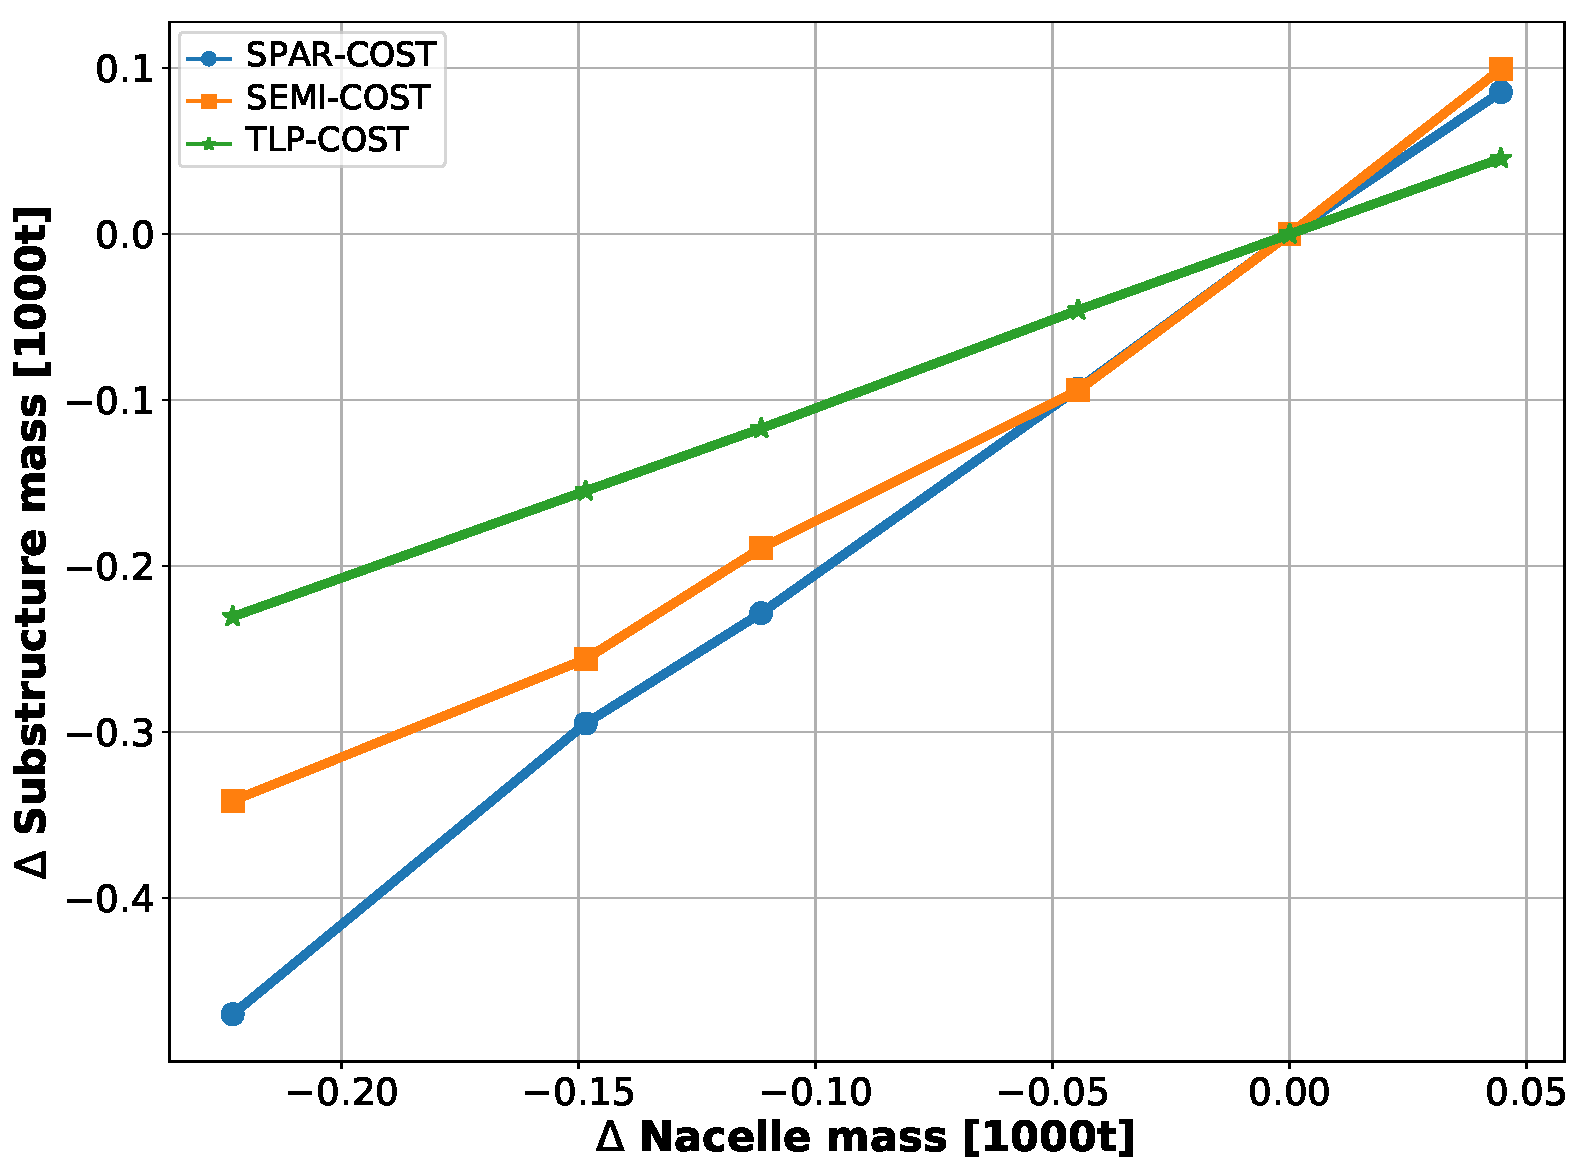
\includegraphics[width=0.9\textwidth]{cost-mass}
    \caption{Absolute mass changes, cost-optimized}
  \end{subfigure}
  \begin{subfigure}[b]{0.49\linewidth}
    \centering 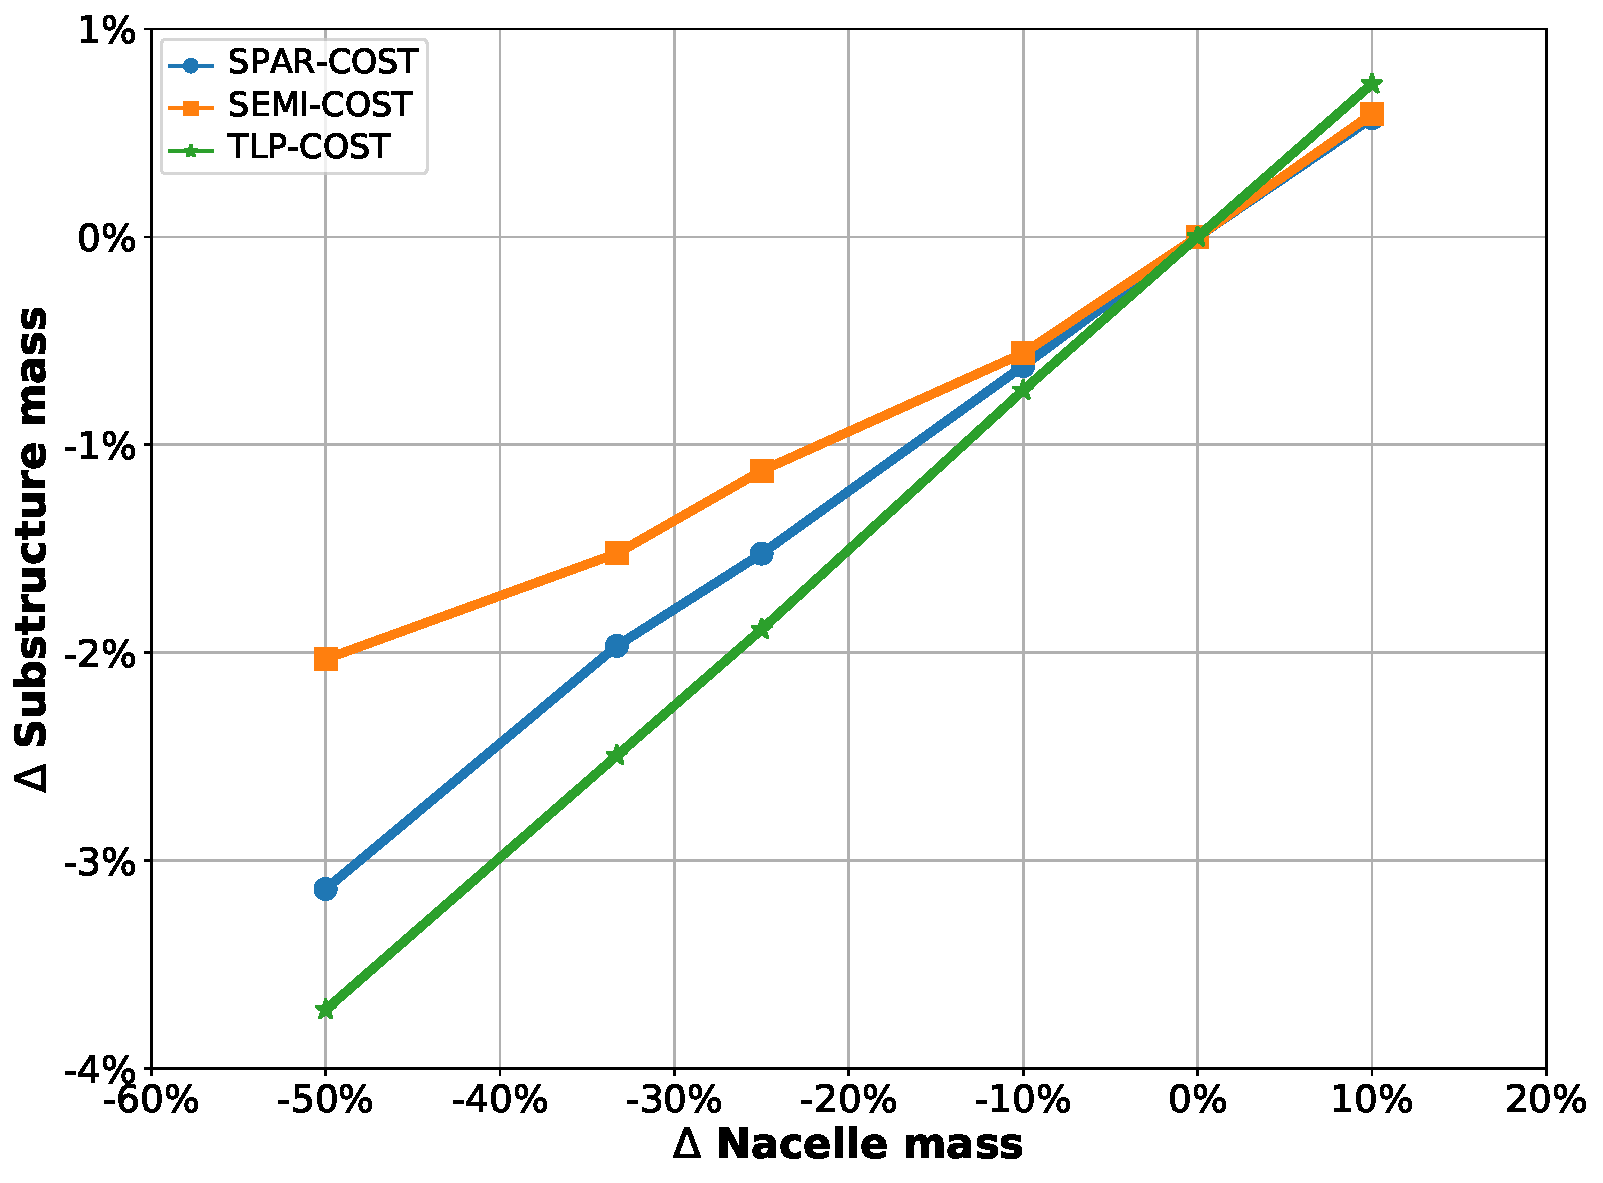
\includegraphics[width=0.9\textwidth]{cost-mass_perc}
    \caption{Percent mass changes, cost-optimized}
  \end{subfigure}\\
  \begin{subfigure}[b]{0.49\linewidth}
    \centering 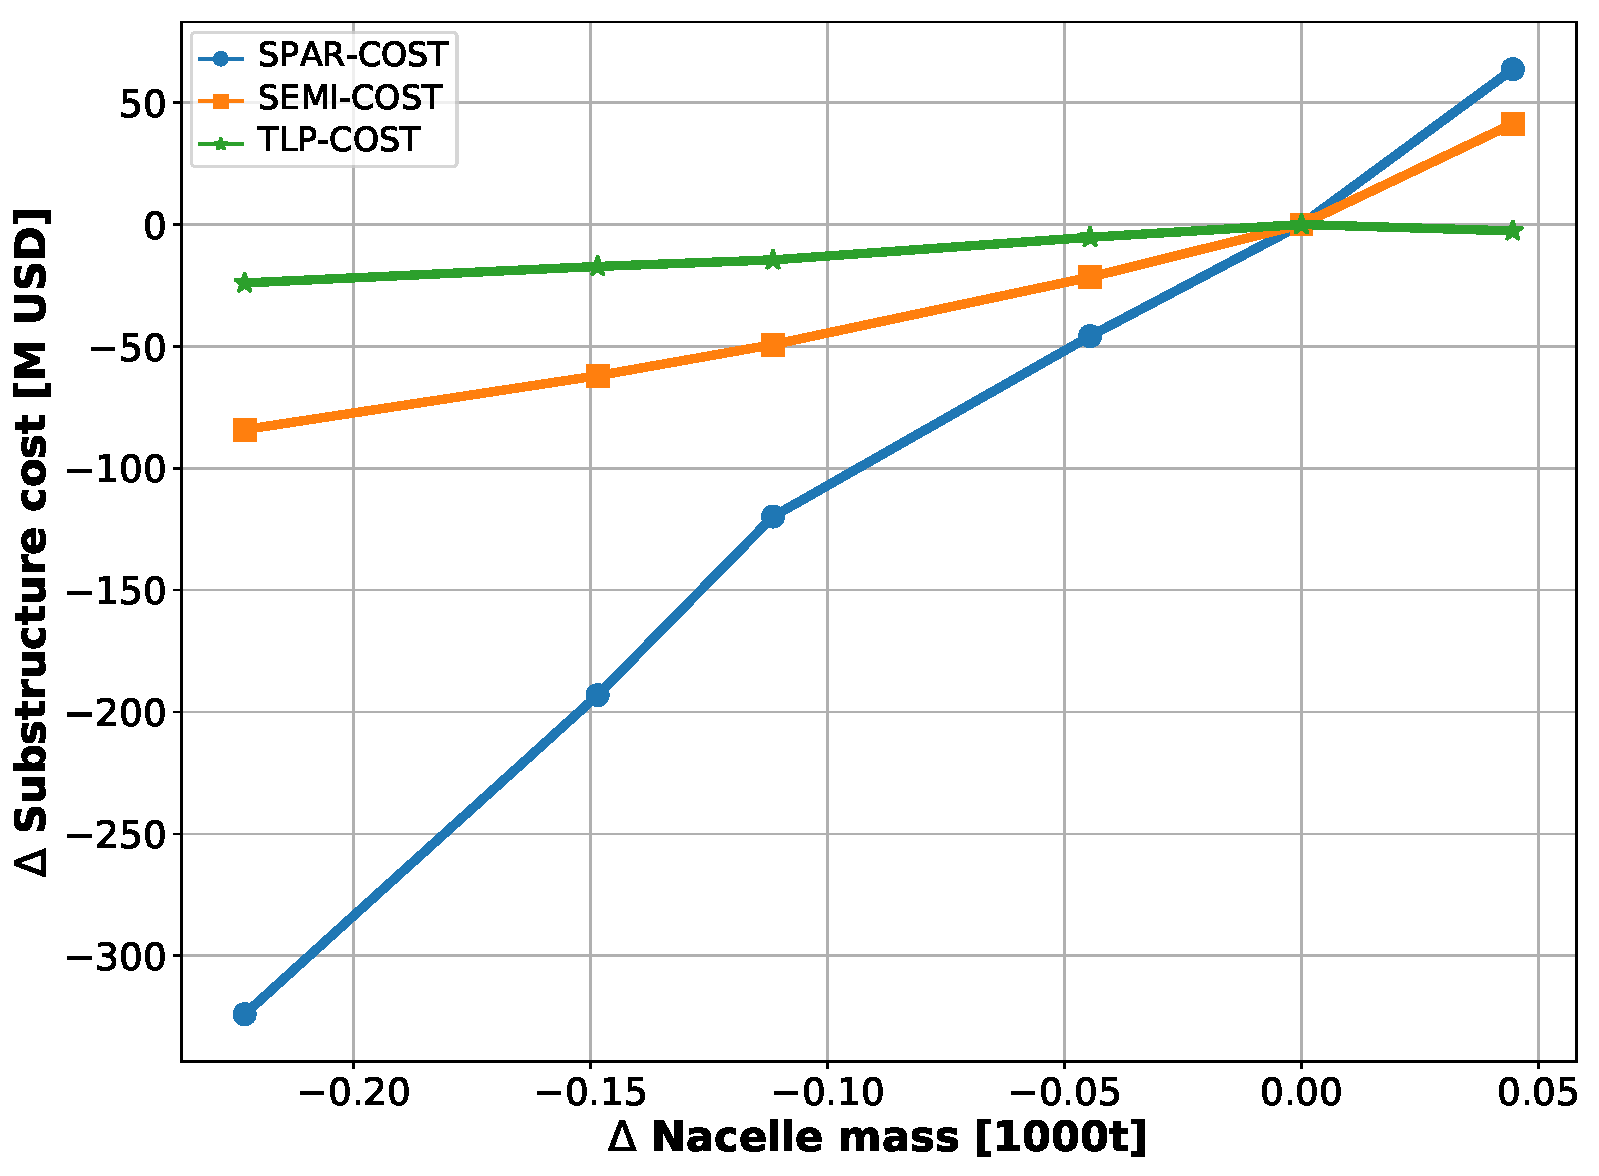
\includegraphics[width=0.9\textwidth]{cost-cost}
    \caption{Absolute cost changes, cost-optimized}
  \end{subfigure}
  \begin{subfigure}[b]{0.49\linewidth}
    \centering 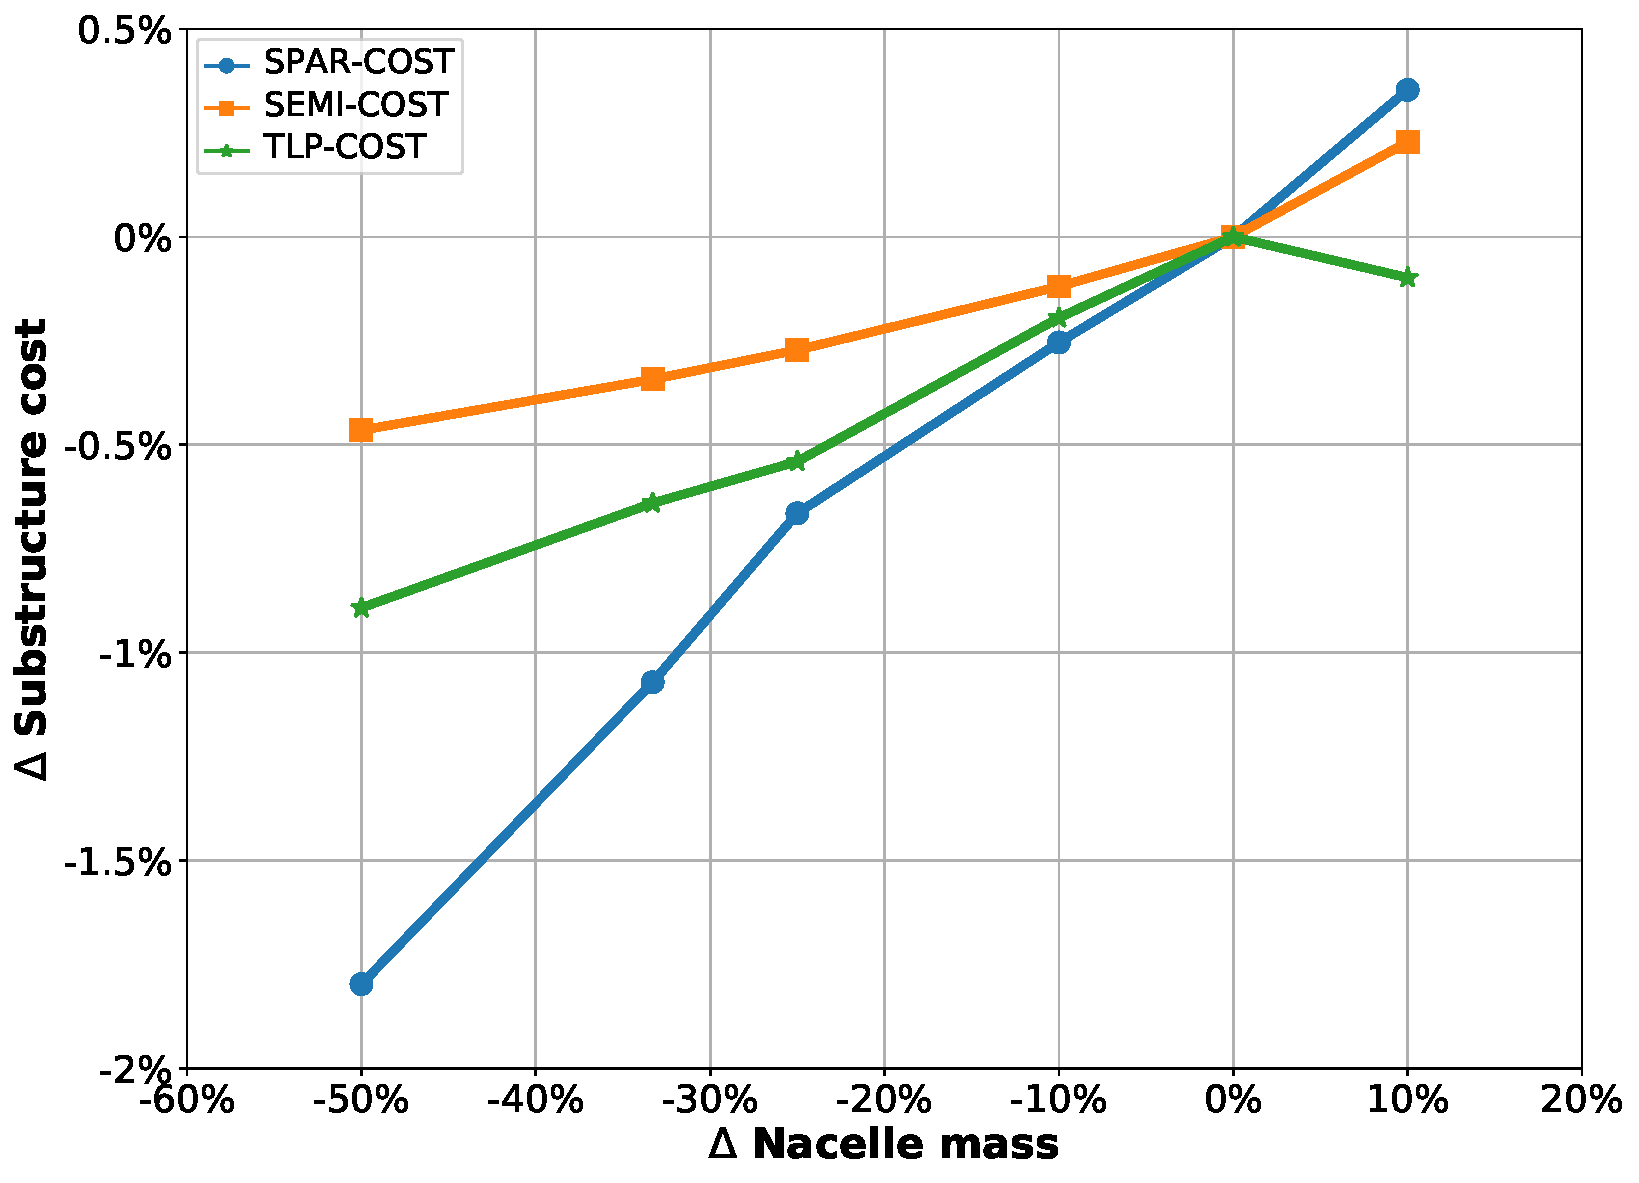
\includegraphics[width=0.9\textwidth]{cost-cost_perc}
    \caption{Percent cost changes, cost-optimized}
  \end{subfigure}
  \caption{Sensitivity of substructure cost (without mooring system)
    relative to mass changes in nacelle for cost-optimized baseline designs.}
  \label{fig:cost-cost}
\end{figure}

The cost reductions for the cost-optimized designs are shown in Figures
\ref{fig:cost-cost}c--d.  Here, at least, there is a consistent cost
decrease, although by percentage it is still far
from the percentage mass decrease.  This is once again explained by the
difference in cost rates among the different components.

The results shown in Figures \ref{fig:mass-cost}-\ref{fig:cost-cost}
have some broader applications than for the immediate study presented
here.  In many engineering studies, mass is used as a surrogate for
capital cost since the development of cost models usually requires a
different set of expertise and input data than what is required for
engineering models.  The implications of the result shown in
Figure \ref{fig:mass-cost} is that mass minimization is not necessarily
a perfect surrogate for capital cost minimization in all cases.  In our
case, the different cost rates for different components means a
mass-focused objective function targets different changes than a
cost-focused objective function.  In other cases, perhaps with
sophisticated cost models that account for various alternative
manufacturing and logistical processes, mass is simply no longer an
adequate surrogate for cost.  Regardless, this observation underscores
some of the messages conveyed in Section \ref{sec:intro} that
advocate for a multidisciplinary systems framework that uses lifecycle
costs to ascertain holistic cost reduction pathways.


\subsection{Break-Even Cost Point for Nacelle Mass Reduction}
One of the more interesting nuggets that can be derived from this type
of design sensitivity study is the cost point required for the
mass-reducing technology (in this case in the drivetrain) to break-even
with the cost changes incurred through the system redesign.  Meaning,
removing mass from the nacelle through the introduction of a new
technology likely comes with a cost premium.  This extra cost, however,
can be offset when the mass savings are propagated through the rest of
the system to reduce structural mass and (hopefully) cost.

\begin{figure}[htbp]
  \begin{center}
    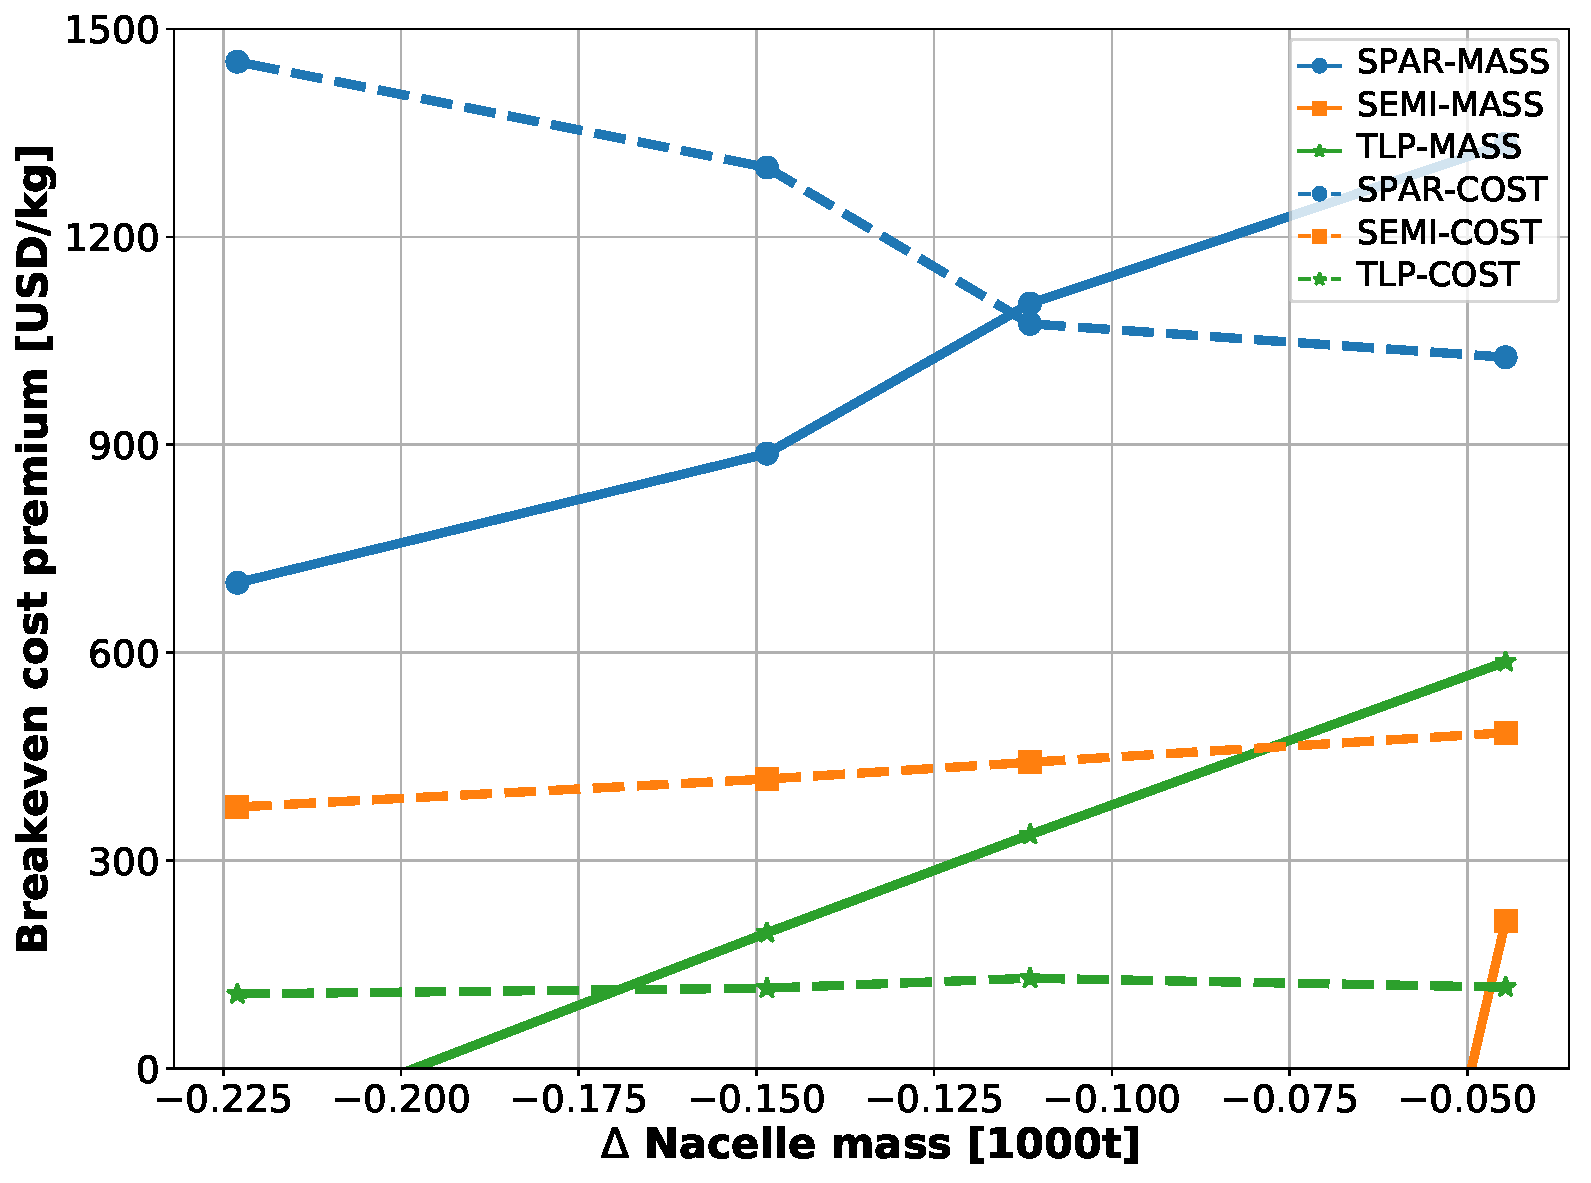
\includegraphics[width=3.5in]{all-premium}
    \caption{Break-even cost premium for the introduction of new drivetrain
      technology.}
    \label{fig:premium}
  \end{center}
\end{figure}

The calculated break-even cost points, for both mass- and cost-optimized
designs, are shown in Figure \ref{fig:premium}.  For the spar designs,
both mass- and cost-optimized, the break-even cost for new drivetrain
technology is approximately \unit[700--1400]{USD/kg}, with a narrower
window for the cost-optimized.  Meaning, if the cost premium to nacelle
mass reduction ratio of the new technology is greater than this value,
then there would be a net cost increase to the system.  If the ratio is
less than this range, then there would be a net cost reduction to the
system.  If the ratio lies within this range, then a little more
detailed investigation would be necessary.

The mass-optimized TLP break-even cost ranges from
\unit[0--600]{USD/kg}, which is a significant variation from
\textit{never worthwhile} to \textit{worthwhile}.  Recall that the cost
reduction in Figure \ref{fig:mass-cost} for the TLP was essentially flat
for reasons already explained.  This is what is driving the inconclusive
determination of the break-even point.  For the same reason, the
mass-optimized semisubmersible design hardly appears in the visual
region of Figure \ref{fig:premium}.

For the cost-optimized semisubmersible and TLP, the break-even results
are much more consistent.  For the semisubmersible, the break-even
cost-ratio is approximately \unit[400--500]{USD/kg} and for the TLP the
value is only about \unit[100]{USD/kg}, a difficult threshold to meet.
Thus, the break-even cost point is dependent on the type of substructure
for this application, hypothetical drivetrain improvement technologies,
and likely other technologies too.


\section{Conclusions}
\label{sec:conc}

This paper has introduced the new WISDEM module, \textit{FloatingSE},
for hydrostatic-based sizing and conceptual design of floating offshore
wind turbine substructures.  To showcase the capabilities of this
module, and the larger WISDEM framework, a two-step analysis was carried
out.  First, three different substructures, a spar, semisubmersible, and
TLP, were designed for the DTU \unit[10]{MW} reference turbine using the
same set of descriptive configuration variables and analysis tools.  This
demonstrates the ability of \textit{FloatingSE} to parametrically
describe entirely different platform architectures that achieve
stability through different underlying mechanisms.  Second, a design
sensitivity study was conducted where mass in the nacelle was
parametrically removed, to simulate the addition of a novel drivetrain
or generator technology, and the design re-optimized.  The derived
sensitivities were used to ascertain the break-even cost rate of the new
technology that reduces the drivetrain mass.

The optimization-based analyses yielded a few interesting, and some
unexpected results.  First, cost reductions in floating offshore wind
energy can be achieved by a consideration of the entire engineering,
manufacturing, and operation requirements concurrently.  Second, mass
can be a poor surrogate for cost in engineering design as due to
differences in cost rates and complexity in cost models.  This
underscores the need for a cost-focused multidisciplinary systems
framework for floating offshore wind.  Finally, the break-even point for
drivetrain technologies that offer mass savings for a cost premium are
approximately \$1,000 for the spar, \$450 for the semisubmersible, and
\$100 for the TLP.

The design sensitivity study was just one of the questions that could be
posed of \textit{FloatingSE} and WISDEM to help answer one of the many
outstanding questions regarding floating offshore wind technology.  Some
of the other questions that could be explored in greater depth include,
\begin{itemize}
\item What are the cost-benefit tradeoffs of a floating substructure
  designed to operate in many different regions versus one that is more
  customized to particular metocean environment?
\item What is the impact on floating systems (e.g., weight, cost,
  scale-ability) due to a new technology?  Is that new
  technology worth the investment?
\item What technologies should governments and industry invest in to
  achieve the greatest cost reduction in floating offshore wind energy?
\item Where can alternative materials, such as composites and concrete,
  be used on the turbine to reduce cost, taking into account regional
  material and labor cost differences?
\end{itemize}

The results presented here were prefaced with many caveats due to the
many simplifying assumptions and low-fidelity analyses within
\textit{FloatingSE}.  Hence, there is significant plans for future
improvements.  Future plans include accounting for hydrodynamics and
additional load cases and a more detailed cost model of the balance of
station and operational costs of an offshore floating wind plant in
WISDEM.  As these improvements are made, the results determined in this
paper may change, perhaps significantly.  Nevertheless, the improvements
on the whole will enable the framework to address a richer set of open
analysis questions with greater certainty.

\section*{Acknowledgments}
The original version of this model was developed by Senu Sirnivas, who
deserves credit for laying out the methodology described here.  The
authors would also like to thank Patrick Gilman, Alana Duerr, Gary
Norton, Daniel Beals, Eric Lantz, and Jason Jonkman for their valuable
input in reviewing results and drafts of this paper.

NREL’s contributions to this work were supported by the US Department of
Energy under Contract Number DE-AC36-08GO28308 with the National
Renewable Energy Laboratory.



% bibliography
%\cleardoublepage
%\label{sec:Bib}
%\printbibliography[heading=bibintoc]

\begin{singlespace} \begin{small} \pagestyle{plain}
    \bibliography{offshore}
    %\bibliographystyle{aiaa}
    %\bibliographystyle{plainnat}
    \bibliographystyle{nattyice-long}
    \addcontentsline{toc}{chapter}{\hspace{3ex}Bibliography}
\end{small} \end{singlespace}


\end{document}

